\documentclass[11pt]{book}
\usepackage[T1]{fontenc}
\usepackage{lmodern}
\usepackage{amsmath,amssymb,mathtools}
\usepackage[a4paper,margin=28mm]{geometry}
\usepackage[strings]{underscore}
\usepackage{hyperref}
\usepackage{graphicx}
\usepackage{float}
\usepackage{tikz}
\usepackage{booktabs,longtable,array}
\hypersetup{
  hidelinks,
  pdftitle={Informational Dynamics of Time},
  pdfauthor={Adrian Lipa},
  pdfsubject={Relational informational dynamics of temporal structure and spacetime closure},
  pdfkeywords={informational dynamics, time, information geometry, retrodiction, Einstein closure}
}
\title{Informational Dynamics of Time}
\author{Adrian Lipa}
\date{\today}
\begin{document}
\frontmatter
\maketitle
% GENERATED LOCAL-BUILD FLAT PART - DO NOT MERGE
\chapter*{Abstract}
\addcontentsline{toc}{chapter}{Abstract}

This work develops a conditional research programme in which temporal structure is constructed from an explicitly declared relational model before spacetime geometry is introduced. The starting data are relational states and directed transitions carrying a normalized probability distribution, a normalized complex representative on phase-bearing sectors, positive transition weights, an ordering parameter distinct from metric clock time, and an inherited dimensionless normalization. The programme then asks which temporal quantities follow from those inputs by definition, exact identity, dynamical closure, or calibrated physical bridge.

Directed transitions carry both an exact Shannon entropy difference and a geometric phase link. Their combination with a separately typed non-exact path-affinity term is used to construct an auditable temporal transition phase, while closed-cycle identities separate exact state-function changes from genuinely non-exact directional information. Positive transition activity then generates an elapsed measure and a relative lapse before a spacetime metric is introduced. Downstream layers develop NOW support, bifurcation, transport, memory, constructive retrodiction, preregistered physical tests, and finally a temporal-to-spacetime closure interface.

The use of the word \emph{derived} is deliberately restricted: IDT does not claim that physical time follows uniquely from Shannon information alone. Its claims are conditional on the declared relational primitives and domains. Standard results from information theory, geometric phase, nonequilibrium response, quantum-state geometry, general relativity, and horizon thermodynamics are treated as imported background or recovery benchmarks rather than as new predictions.

Formal derivation, computational evidence, and physical claim status are maintained as separate layers. Exact identities, reference-model reconstructions, calibrated physical correspondences, and replicated measured results are not interchangeable evidence classes. The strongest present results are constructive and algebraic within their stated domains; the strongest physical claims remain attached to explicit falsification protocols whose calibration variables and null models are fixed independently of the measured outcome.

% GENERATED LOCAL-BUILD FLAT PART - DO NOT MERGE
\chapter*{Methodological Note}
\addcontentsline{toc}{chapter}{Methodological Note}

The dependency rule of this programme is
\[
\boxed{\text{derive temporal structure first; introduce spacetime later}.}
\]
The construction first imports the TIR relational root
\[
\mathfrak Z_{\rm rel}
\to\mathcal P
\to\{N,S\}
\to\frac12
\to\ln2
\to\mathbb C^2,
\]
without identifying relational zero with a time coordinate, vacuum state, or initial event. IDT-local construction begins only after that upstream packet is admitted, from relational information and phase transport. Each new temporal object is admitted only after its upstream dependencies are explicit. The intended order is
\[
\begin{aligned}
\text{TIR relational root}
&\to\text{information}
\to\text{directed transition}
\to\text{phase structure}
\to\text{temporal state}\\
&\to\text{NOW/bifurcation}
\to\text{transport/memory}
\to\text{metric calibration}\\
&\to\text{space}
\to\text{Einstein closure}.
\end{aligned}
\]

Mathematical construction, computational evidence, and physical claim status are kept distinct. A candidate is first assigned typed variables, equations, dependencies, and falsification conditions. Algebraic identities are proved where possible; numerical controls are used where analytic closure is not yet available. Only then can a claim move to a stronger registry status.

The ordering parameter used in the early formalism is kept distinct from metric clock time. Metric calibration is therefore a downstream bridge rather than a hidden starting assumption. Likewise, chirality, topology, fractal scaling, memory, and subjective temporal accumulation are treated as derived-property targets with their own observables and tests.

\section*{Prior-art and novelty discipline}

Whenever the construction invokes an established object, the corresponding chapter cites the standard source or a primary historical reference. Shannon entropy, Kullback--Leibler divergence, Pancharatnam/Berry phase, Onsager response, reversible Markov entropy gradients, Noether conservation, Einstein gravity, Bell/CHSH tests, and Hawking/Gibbons--Hawking horizon thermodynamics are therefore treated as external scientific context rather than as IDT discoveries.

A statement is called \emph{IDT-specific} only when it depends on the programme's own typed composition, decoder, activity measure, memory carrier, calibration map, or falsification rule. Recovery of a known physical equation is labelled a recovery benchmark. A physical discriminator requires an independently determined IDT quantity that can be evaluated before the target measurement is inspected.

\section*{Falsification before promotion}

For a proposed physical correspondence, the calibration map and null model must be fixed independently of the target outcome. If the same measured quantity is used both to define the IDT predictor and to confirm it, the exercise is classified as calibration or consistency checking rather than discrimination. Promotion to a physical result requires immutable raw data, uncertainty propagation, declared exclusions, and independent replication where the claim warrants it.
% GENERATED LOCAL-BUILD FLAT PART - DO NOT MERGE
\chapter*{Scope, Primitives, and Claim Semantics}
\addcontentsline{toc}{chapter}{Scope, Primitives, and Claim Semantics}

\section*{What is and is not being derived}

Throughout this monograph, the word \emph{derived} has a conditional mathematical meaning. Temporal structures are derived from a declared relational model and its typed primitives; they are not claimed to follow uniquely from Shannon information alone, nor is the existence of physical time inferred from an information measure without additional assumptions.

Before any IDT-local temporal object is introduced, the branch imports the typed TIR relational root
\[
\boxed{
\mathfrak Z_{\rm rel}=(\varnothing,\varnothing)
\to\mathcal P
\to\{N,S\}
\to\frac12
\to\ln2
\to\mathbb C^2.
}
\]
Here \(\mathfrak Z_{\rm rel}\) is a pre-object dependency boundary, not \(t=0\), not a vacuum state, and not an initial event. Conditional on that imported root, the IDT-local temporal branch admits the following objects:
\begin{enumerate}
\item a set of relational states and admitted directed transitions;
\item a normalized probability vector \(p(s)\) on each state, with Shannon entropy \(H_S\);
\item a normalized complex representative \(\psi(s)\) on sectors where phase transport is defined;
\item positive admitted transition probabilities or rates, together with declared relational mobility fields;
\item an ordering parameter \(\lambda\), which is \emph{not} metric clock time;
\item the inherited normalization \(\kappa=\ln 2/(24\pi)\).
\end{enumerate}

From those inputs the programme asks which further structures follow by definition, algebraic identity, dynamical closure, or experimentally testable bridge. The positive elapsed measure, relative lapse, memory carriers, retrodiction maps, and later spacetime interface are therefore downstream constructions whose validity is conditional on their stated domains and dependencies.

\section*{Standard ingredients and the IDT-specific composition}

Several ingredients used in the construction are standard and are not presented as new results. These include Shannon entropy \cite{Shannon1948}, Kullback--Leibler divergence \cite{KullbackLeibler1951}, Pancharatnam/Berry geometric phase \cite{Pancharatnam1956,Berry1984}, quantum-state information geometry \cite{ProvostVallee1980}, Onsager reciprocity and nonequilibrium network structure \cite{Onsager1931,Schnakenberg1976}, and entropy-gradient formulations for reversible finite Markov chains \cite{Maas2011}. The relativistic closure layer likewise uses standard Noether and Einstein structures \cite{Noether1971,Einstein1916}.

The programme-specific content is the typed way these ingredients are composed and constrained: the separation of exact state entropy from non-exact path affinity, the positive-activity temporal measure, the clock-ratio and memory interfaces, the constructive retrodiction carrier, the evidence-class firewall between retrodiction and retrocausal claims, and the explicit temporal-to-spacetime closure gates. A standard identity remains standard even when it is used as an important recovery target inside this architecture.

\section*{Evidence classes}

Every substantive statement belongs to one of five evidence classes:
\[
\boxed{
\begin{array}{c}
\text{definition / admitted primitive}\\
\downarrow\\
\text{proved identity on a declared domain}\\
\downarrow\\
\text{reference-model or software result}\\
\downarrow\\
\text{calibrated physical correspondence}\\
\downarrow\\
\text{replicated measured physical result}.
\end{array}}
\]
A result does not move upward merely because more unit tests pass. Hosted tests establish implementation consistency and regression protection; they are not independent physical observations.

\section*{Theory map}

The monograph follows four layers:
\[
\boxed{
\begin{aligned}
\textbf{I. Foundations:}\quad&
\text{TIR relational root}
\to
\text{relational state}
\to
\text{information + phase}
\to
\text{positive temporal activity},
\\[1mm]
\textbf{II. Temporal dynamics:}\quad&
\text{elapsed measure}
\to
\text{NOW/bifurcation}
\to
\text{transport + memory},
\\[1mm]
\textbf{III. Inference and experiment:}\quad&
\text{retrodiction}
\to
\text{withheld-variable tests}
\to
\text{preregistered physical tests},
\\[1mm]
\textbf{IV. Spacetime closure:}\quad&
\text{temporal coframe}
\oplus
\text{independent spatial/source branch}
\to
\text{Einstein interface}.
\end{aligned}}
\]

This map also fixes the novelty boundary. Standard-physics relations used at Layer IV are recovery benchmarks unless the temporal branch supplies an independently determined quantity that can disagree with the standard prediction before the measurement is inspected.
% GENERATED LOCAL-BUILD FLAT PART - DO NOT MERGE
\chapter*{Notation and Principal Symbols}
\addcontentsline{toc}{chapter}{Notation and Principal Symbols}

\small
\setlength{\LTpre}{0pt}
\setlength{\LTpost}{0pt}
\begin{longtable}{p{0.20\textwidth}p{0.27\textwidth}p{0.43\textwidth}}
\toprule
\textbf{Symbol} & \textbf{Type / domain} & \textbf{Role} \\
\midrule
\endfirsthead
\toprule
\textbf{Symbol} & \textbf{Type / domain} & \textbf{Role} \\
\midrule
\endhead
\(s,a,b\) & relational states & State labels; \(a\to b\) denotes an admitted directed transition. \\
\(p(s)\) & probability simplex & Normalized state probability vector. \\
\(H_S(s)\) & bits & Shannon entropy of \(p(s)\). \\
\(\Delta H_e\) & bits & Exact state-function entropy difference along edge \(e\). \\
\(\psi(s)\) & normalized complex vector & Complex representative used for phase transport. \\
\(G_{a\to b}\) & \(U(1)\) & Normalized Pancharatnam link on a non-orthogonal pair. \\
\(\gamma_B(C)\) & angle & Closed-cycle geometric holonomy. \\
\(\sigma_e\) & bits & Non-exact directional information increment / path affinity. \\
\(\kappa\) & dimensionless & Inherited normalization \(\ln2/(24\pi)\). \\
\(L_e\) & \(U(1)\) & Shannon--phase temporal transition link. \\
\(q_e\) & angle & Argument of \(L_e\); transition phase weight. \\
\(\rho_R,\eta_R\) & positive relational fields & Density- and viscosity-like fields controlling the symmetric mobility sector. \\
\(M_{ab}\) & positive scalar & Symmetric pair mobility. \\
\(W_{a\to b}\) & positive rate & Directed transition rate. \\
\(\mathfrak a\) & positive rate & Symmetric activity \(W_++W_-\); generator of elapsed measure. \\
\(\mathfrak j\) & signed rate & Antisymmetric current \(W_+-W_-\). \\
\(\lambda\) & ordering coordinate & Monotone ordering parameter; not metric clock time. \\
\(\Theta\) & elapsed activity measure & Primitive accumulated temporal measure with \(d\Theta=\mathfrak a\,d\lambda\). \\
\(N_R(x|r)\) & positive ratio & Relative lapse / clock-rate ratio \(\mathfrak a_x/\mathfrak a_r\). \\
\(\Phi(N_R)\) & dimensionless & Relative-information clock potential \(N_R-1-\ln N_R\). \\
\(\widehat\tau\) & calibrated time & Physical elapsed time after reference-clock calibration. \\
\(m\) & complex memory coordinate & Two-component memory carrier used in the reference reconstruction class. \\
\(\Delta M_n\) & operator difference & Projective pre/post event memory imprint. \\
\(\alpha\) & ordered index packet & Active-attractor sequence in the stratified decoder. \\
\(\mathcal W\) & winding packet & Oriented winding lineage retained by the compressed decoder. \\
\(\rho_k\) & positive radius & Radial coordinate relative to the active attractor. \\
\(\Theta_R\) & length-valued one-form & Relativistic temporal coframe input \(N_Rc\,dt\). \\
\(g_{\mu\nu}\) & spacetime metric & Introduced only at the downstream spacetime closure layer. \\
\(T_{\mu\nu}\) & stress-energy tensor & Physical source ledger at the Einstein interface. \\
\(\kappa_E\) & gravitational coupling & Standard \(8\pi G/c^4\); not derived anew by IDT. \\
\(\kappa_H\) & surface gravity scale & Horizon parameter used in the standard Euclidean thermal benchmark. \\
\bottomrule
\end{longtable}
\normalsize

Symbols introduced only inside a specialised decoder, experiment, or source adapter are defined locally in the corresponding chapter. Reuse of a symbol in a different typed domain is avoided where it would change the meaning of an established quantity.

\tableofcontents
\mainmatter
\part{Foundations and Temporal Construction}
% GENERATED LOCAL-BUILD FLAT PART - DO NOT MERGE
\chapter{TIR Entrypoint}

The temporal branch does not begin from a physical time coordinate. It imports only registry-declared TIR objects and preserves their dependency order.

The upstream relational root is
\[
\boxed{
\mathfrak Z_{\rm rel}
=
(\varnothing,\varnothing)
\longrightarrow
\mathcal P=\{p\}
\longrightarrow
\Pi_1=\{N,S\}
\longrightarrow
\frac12
\longrightarrow
\ln2
\longrightarrow
\mathbb C^2.
}
\]

Here $\mathfrak Z_{\rm rel}$ is the TIR empty relational presentation. It is not a point and is not a temporal coordinate. In particular,
\[
\boxed{
0_{\rm rel}
\neq
t=0
\neq
\tau_{\rm int}=0
\neq
\text{vacuum state}
\neq
\text{initial event}.
}
\]
The point is the minimal nonempty support downstream of relational zero. The first binary distinction is the minimal nontrivial distinction; exchange symmetry then fixes the normalized share $1/2$, and Shannon information gives $\ln2$.

IDT imports this root rather than re-deriving or reinterpreting it. The typed cross-repository contract is maintained in
\path{formalism/00A_tir_relational_zero_entrypoint.md}.

The canonical TIR normalization used downstream in IDT is
\[
\kappa=\frac{\ln2}{24\pi}.
\]
Its denominator and flavour/mixing ownership remain TIR-side dependencies; IDT does not promote the normalization from the zero layer alone.

The first local temporal construction combines three typed objects rather than collapsing them into one: Shannon state entropy $H_S$, geometric phase transport $G_e$, and a transition-associated non-exact information-production increment $\sigma_e$.

The dependency chain at this stage is therefore
\[
\boxed{
\text{TIR relational root}
\longrightarrow
\text{relational state}
\longrightarrow
(H_S,\psi)
\longrightarrow
(\Delta H_e,G_e)
\longrightarrow
L_e
\longrightarrow
q_e
\longrightarrow
\mathcal K_T.
}
\]

The first explicit candidate closure of the edge quantity is
\[
\sigma_{a\to b}=\log_2\frac{P(b\mid a)}{P(a\mid b)}.
\]
This closes the free edge parameter at the information-theoretic level while preserving the distinction between state entropy and path affinity. The next upstream debt is to derive the forward/reverse transition weights from the relational density and viscosity fields rather than supplying them externally.

The publication firewall is:
\[
\boxed{
\text{relational zero}
\not\Rightarrow
\text{physical time};
\qquad
\text{TIR structural import}
\not\Rightarrow
\text{IDT empirical promotion}.
}
\]

% GENERATED LOCAL-BUILD FLAT PART - DO NOT MERGE
\chapter{Information and Relational Order}

The temporal programme begins from relational states rather than from a pre-existing time coordinate. Each state $s$ is assigned a probability distribution
\[
p(s)=(p_1,\ldots,p_m),
\qquad
p_i\geq0,
\qquad
\sum_i p_i=1,
\]
and its Shannon entropy in bits \cite{Shannon1948},
\[
\boxed{
H_S(s)=-\sum_i p_i(s)\log_2p_i(s).
}
\]
The inherited normalization is
\[
\kappa=\frac{\ln2}{24\pi}.
\]

For an admitted directed transition $e:a\to b$, the first informational quantity is the exact state-function difference
\[
\Delta H_e=H_S(b)-H_S(a).
\]
This quantity measures the change in the Shannon state entropy across that transition. Importantly, it is an exact difference. Therefore, for every closed directed cycle $C$,
\[
\boxed{
\sum_{e\in C}\Delta H_e=0.
}
\]
The identity follows by telescoping and has a direct methodological consequence: a state entropy difference can contribute to an open transition, but it cannot by itself generate a non-zero circulation around a closed cycle.

\section{Complex relational state and phase transport}

The same relational state is also represented by a normalized complex vector
\[
\psi(s)\in\mathbb C^m,
\qquad
\langle\psi|\psi\rangle=1.
\]
Whenever two consecutive states have non-zero overlap, define the normalized Pancharatnam link, following the standard geometric-phase construction \cite{Pancharatnam1956,Berry1984},
\[
G_{a\to b}
=
\frac{\langle\psi_a|\psi_b\rangle}
{|\langle\psi_a|\psi_b\rangle|}
\in U(1).
\]
An open link is gauge-covariant under local rephasing of the state representatives. The ordered product of links around a closed cycle is gauge-invariant and defines the discrete geometric holonomy
\[
\gamma_B(C)
=
\operatorname{Arg}\!\left(\prod_{e\in C}G_e\right).
\]

\section{Shannon--phase transition link}

To connect informational change and phase transport without identifying them prematurely, introduce a transition-associated non-exact information increment $\sigma_e$. The first microscopic candidate closure is obtained from forward/reverse transition asymmetry. Log-ratios of directed transition weights and their cycle affinities are standard objects in network nonequilibrium thermodynamics \cite{Schnakenberg1976}; the IDT-specific step is their typed coupling to the temporal phase link. For strictly positive admitted transition probabilities,
\[
\boxed{
\sigma_{a\to b}
=
\log_2\frac{P(b\mid a)}{P(a\mid b)}.
}
\]
This quantity is path-level rather than a state entropy. It obeys $\sigma_{b\to a}=-\sigma_{a\to b}$ and vanishes for a symmetric transition pair. The candidate temporal link is
\[
\boxed{
L_e
=
G_e\exp\!\left[i\kappa\left(\Delta H_e+\sigma_e\right)\right].
}
\]
The corresponding transition phase weight is
\[
q_e=\operatorname{Arg}L_e.
\]
It can therefore enter the atomic temporal transition measure used later in the construction,
\[
\mathcal K_T=\sum_e q_e\,\delta_{s_e}.
\]

For a closed cycle the exact Shannon contribution cancels. Defining the cycle affinity
\[
\mathcal A_C
=
\sum_{e\in C}\sigma_e
=
\log_2\prod_{e\in C}
\frac{P_{e,+}}{P_{e,-}},
\]
gives
\[
\boxed{
\operatorname{Arg}\!\left(\prod_{e\in C}L_e\right)
=
\gamma_B(C)
+
\kappa\mathcal A_C
\pmod{2\pi}.
}
\]
This is the first structural separation in the derivation. The geometric part supplies phase holonomy. The exact Shannon state potential supplies open-transition information change. Directed path affinity supplies a non-exact information channel that can survive cycle closure.

A useful control follows immediately. If a strictly positive relational weight $\pi_s$ satisfies pairwise detailed balance,
\[
\pi_aP(b\mid a)=\pi_bP(a\mid b),
\]
then
\[
\sigma_{a\to b}=\log_2\frac{\pi_b}{\pi_a}
\]
and the cycle affinity telescopes to zero. Non-zero $\mathcal A_C$ is therefore a precise obstruction to this detailed-balance representation on the declared cycle.

\section{Relational density, viscosity, and mobility}

Let the relational state carry strictly positive scalar fields $\rho_R(s)$ and $\eta_R(s)$. The minimal pair mobility used here is
\[
\boxed{
M_{ab}
=
\frac{\sqrt{\rho_R(a)\rho_R(b)}}
{\tfrac12[\eta_R(a)+\eta_R(b)]}.
}
\]
It is symmetric under $a\leftrightarrow b$. To keep pace and direction as separate typed quantities, introduce an antisymmetric dimensionless edge drive
\[
A_{ab}=-A_{ba}
\]
and define
\[
\boxed{
W_{a\to b}=M_{ab}e^{A_{ab}/2},
\qquad
W_{b\to a}=M_{ab}e^{-A_{ab}/2}.
}
\]
Then
\[
\sigma_{a\to b}
=
\log_2\frac{W_{a\to b}}{W_{b\to a}}
=
\frac{A_{ab}}{\ln2}.
\]
The symmetric mobility cancels from the directional ratio. Thus, in this minimal construction, relational density and viscosity control transition pace while the antisymmetric edge drive controls directional affinity.

A second structural control follows. If the edge drive is an exact state-potential difference,
\[
A_{ab}=V_R(b)-V_R(a),
\]
then its closed-cycle sum vanishes. Therefore a non-zero temporal circulation requires a non-exact edge drive or an enlarged state in which memory/history changes the relevant transition geometry.

The rate pair also admits a symmetric/antisymmetric decomposition,
\[
\mathfrak a_{ab}=W_{a\to b}+W_{b\to a},
\qquad
\mathfrak j_{ab}=W_{a\to b}-W_{b\to a}.
\]
The activity $\mathfrak a_{ab}$ is strictly positive and invariant under edge reversal, while the current $\mathfrak j_{ab}$ reverses sign. This decomposition will be used in the NOW layer to distinguish event existence from directional current.

The next derivational target is consequently sharper: identify whether memory-orbit state, phase holonomy, or another admitted relational structure generates the non-exact part of $A_{ab}$, while $\rho_R$ and $\eta_R$ regulate the pace of realization.

% GENERATED LOCAL-BUILD FLAT PART - DO NOT MERGE
\chapter{Kähler Information Geometry}
The temporal construction begins on a state/information manifold \(\mathcal M\). Spacetime coordinates enter later at Einstein Closure.

\section{Relational forcing of the local geometry}
A positive context-sensitive internal elapsed measure has the local form
\[
 d\tau_{\rm int}=\phi(x,\lambda)\,d\lambda,
 \qquad \phi>0,
\]
so the scalar temporal pace is the Radon--Nikodym density of internal elapsed time with respect to the ordering parameter. In the current kinetic realization,
\[
\boxed{\phi=\frac{\mathfrak a}{\mathfrak a_\star}.}
\]

For a scalar informational functional \(\mathcal I\), the differential \(d\mathcal I\) is a covector. Coordinate-covariant local linear response therefore introduces a contravariant rank-two tensor \(G^{AB}\):
\[
V_I^A=-G^{AB}\partial_B\mathcal I.
\]
Positive informational descent makes the symmetric response positive semidefinite. On each active nondegenerate tangent sector it defines the inverse metric response.

A reversible phase response generated locally by \(\mathcal H_\alpha\) takes the form
\[
V_H^A=\Omega^{AB}\partial_B\mathcal H_\alpha,
\]
and preservation of \(\mathcal H_\alpha\) for arbitrary admitted phase covectors makes \(\Omega^{AB}\) antisymmetric. With the admitted unit \(U(1)\) phase generator \(J\),
\[
J^2=-I,
\qquad
\Omega^{AB}=J^A{}_{C}G^{CB},
\]
which yields the local exact-patch factorization
\[
\boxed{
\frac{dx}{d\lambda}
=-\operatorname{grad}_{g_K}\mathcal I
+J\operatorname{grad}_{g_K}\mathcal H_\alpha.
}
\]

\section{Shannon--Onsager realization of the symmetric response}
Formalism 01C fixes the stationary-reference informational scalar to the Kullback--Leibler divergence \cite{KullbackLeibler1951},
\[
\boxed{
\mathcal I_\pi[p]=D_{\rm KL}^{(2)}(p\|\pi).
}
\]
For an admitted stationary Markov kernel, data processing gives
\[
\mathcal I_\pi[pP]\le\mathcal I_\pi[p].
\]
The use of an informational potential in a dissipative response is consistent with the Onsager framework \cite{Onsager1931}; finite-state reversible Markov chains also admit rigorous entropy-gradient-flow formulations \cite{Maas2011}. The tensor below is the specific response adopted by the present formalism. In the continuous-time detailed-balance sector, let
\[
c_{ab}=\pi_aQ_{ab}=\pi_bQ_{ba},
\qquad
r_a=\frac{p_a}{\pi_a},
\]
and define the logarithmic mean
\[
\Lambda(x,y)=\frac{x-y}{\ln x-\ln y}.
\]
The exact symmetric response tensor is
\[
\boxed{
G^{(2)}_\pi(p)
=(\ln2)D^\top
\operatorname{diag}[c_{ab}\Lambda(r_a,r_b)]D,
}
\]
with
\[
\boxed{
\dot p=-G^{(2)}_\pi(p)\nabla_p\mathcal I_\pi.
}
\]
It obeys
\[
G^{(2)}_\pi\mathbf1=0,
\]
so the constant covector is the mass-conservation null. For a connected response graph, the metric is defined on the probability-simplex tangent quotient.

In the uniform zero-drive relational sector,
\[
\boxed{
G^{(2)}_u(u)=\frac{\ln2}{m}K_0,
\qquad
K_0=D^\top\operatorname{diag}(M_{ab})D.
}
\]
Thus the symmetric information geometry and the later Temporal Wave stiffness share the same relational-mobility Laplacian at uniform equilibrium.

\section{Global phase connection and holonomy}
The Shannon--Pancharatnam primitive assigns each admitted edge
\[
L_e=G_e\exp\!\left[i\kappa(\Delta H_e+\sigma_e)\right].
\]
Exact scalar differences obey \(\sum_C\Delta H_e=0\), while the closed-cycle temporal phase is
\[
\boxed{
\Phi_T(C)=\gamma_B(C)+\kappa\sum_{e\in C}\sigma_e\pmod{2\pi}.
}
\]
Admitted nonzero \(\Phi_T\) is carried globally by the temporal \(U(1)\) connection and its holonomy. The scalar \(\mathcal H_\alpha\) remains the local generator on an exact patch; the connection supplies the transition and cycle data needed to patch those local descriptions across the state bundle.

The associated two-form is
\[
\omega(X,Y)=g_K(JX,Y).
\]
The complex-projective/Fubini--Study sectors used by the Memory construction follow the standard quantum-state geometry \cite{ProvostVallee1980}, while the admitted geometric-phase sector is connected to the Pancharatnam--Berry construction \cite{Pancharatnam1956,Berry1984}. On compatible active sectors the resulting package
\[
\boxed{(\mathcal M,J,g_K,\omega)}
\]
is Kähler under the declared compatibility and closure conditions.

For an oriented two-chain \(\Sigma\), the signed Kähler-area diagnostic
\[
\mathcal A_K[\Sigma]=\int_\Sigma\omega
\]
obeys
\[
\mathcal A_K[-\Sigma]=-\mathcal A_K[\Sigma].
\]
This gives the formalism an orientation-sensitive geometric object. Temporal chirality is then tested downstream by the dynamics and holonomy gates.

\section{Visual phase portrait}
Figure~\ref{fig:kahler-flow-2d} gives a schematic 2D slice of the Kähler time flow. The nested contours represent levels of the informational functional; representative trajectories combine inward informational descent with the transverse phase response.
\begin{figure}[H]
  \centering
  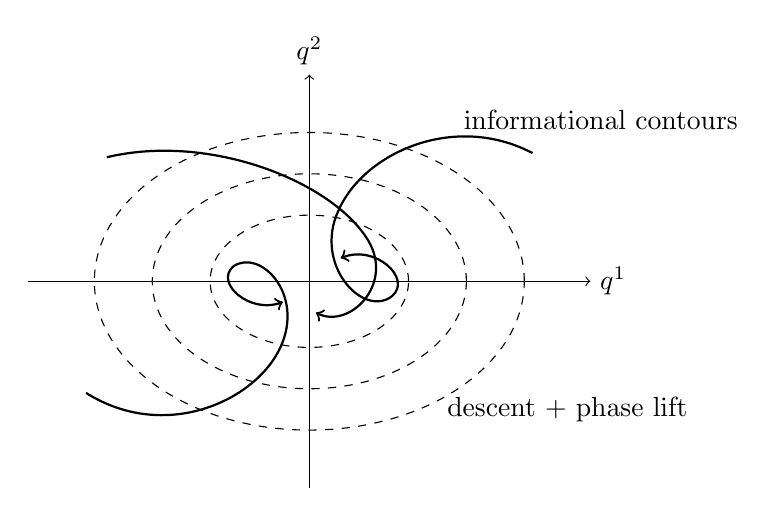
\begin{tikzpicture}[scale=1.05]
    \draw[->] (-3.4,0) -- (3.4,0) node[right] {$q^1$};
    \draw[->] (0,-2.5) -- (0,2.5) node[above] {$q^2$};
    \draw[dashed] (0,0) ellipse (2.6 and 1.8);
    \draw[dashed] (0,0) ellipse (1.9 and 1.3);
    \draw[dashed] (0,0) ellipse (1.2 and 0.8);
    \draw[->,thick] (2.7,1.55)
      .. controls (1.75,2.05) and (0.65,1.55) .. (0.35,0.85)
      .. controls (0.05,0.20) and (0.65,-0.45) .. (1.00,-0.18)
      .. controls (1.25,0.03) and (0.80,0.45) .. (0.38,0.28);
    \draw[->,thick] (-2.7,-1.35)
      .. controls (-1.75,-1.95) and (-0.65,-1.45) .. (-0.35,-0.80)
      .. controls (-0.05,-0.15) and (-0.60,0.40) .. (-0.92,0.18)
      .. controls (-1.15,-0.02) and (-0.72,-0.40) .. (-0.32,-0.25);
    \draw[->,thick] (-2.45,1.50)
      .. controls (-1.20,1.80) and (0.30,1.20) .. (0.72,0.48)
      .. controls (1.02,-0.05) and (0.48,-0.58) .. (0.08,-0.38);
    \node[anchor=west] at (1.75,1.95) {informational contours};
    \node[anchor=west] at (1.55,-1.55) {descent + phase lift};
  \end{tikzpicture}
  \caption{Schematic two-dimensional Kähler time-flow slice with informational level contours and representative trajectories combining symmetric descent with the transverse phase response.}
  \label{fig:kahler-flow-2d}
\end{figure}

% GENERATED LOCAL-BUILD FLAT PART - DO NOT MERGE
\chapter{Tensor--Scalar Temporal Field}
The temporal configuration is represented by a scalar pace together with a rank-two relational response sector. The scalar component is typed by the internal elapsed density
\[
\boxed{
\phi
=\frac{d\tau_{\rm int}}{d\lambda}
=\frac{\mathfrak a}{\mathfrak a_\star}>0.
}
\]
For the same ordering increment \(d\lambda\), distinct admitted relational states may therefore realize distinct internal elapsed increments.

The tensorial response is written locally as
\[
\boxed{
\mathcal R^{AB}=G^{AB}+\Omega^{AB},
}
\]
where
\[
G^{AB}=G^{BA},
\qquad
\Omega^{AB}=-\Omega^{BA}.
\]
The symmetric positive sector maps the informational covector to dissipative state transport,
\[
V_I^A=-G^{AB}\partial_B\mathcal I,
\]
while the antisymmetric sector maps a local exact phase covector to reversible state transport,
\[
V_H^A=\Omega^{AB}\partial_B\mathcal H_\alpha.
\]

Formalism 01C supplies the stationary Shannon informational scalar
\[
\boxed{
\mathcal I_\pi[p]=D_{\rm KL}^{(2)}(p\|\pi).
}
\]
For admitted stationary transition dynamics this scalar contracts. In the detailed-balance sector, Formalism 01D derives the exact symmetric response
\[
\boxed{
G^{(2)}_\pi(p)
=(\ln2)D^\top\operatorname{diag}[c_{ab}\Lambda(r_a,r_b)]D,
\qquad
r_a=\frac{p_a}{\pi_a},
}
\]
and the exact flow identity
\[
\boxed{
\dot p=-G^{(2)}_\pi(p)\nabla_p\mathcal I_\pi.
}
\]
The mass-conservation direction satisfies
\[
G^{(2)}_\pi\mathbf1=0,
\]
so the corresponding metric response is taken on the active simplex tangent quotient. At uniform zero-drive equilibrium,
\[
\boxed{
G^{(2)}_u(u)=\frac{\ln2}{m}K_0,
}
\]
which ties the symmetric information-response tensor directly to the relational-mobility Laplacian used by Temporal Wave.

In the admitted Kähler factorization on a compatible active sector,
\[
g_{K,AB}=(G^{-1})_{AB},
\qquad
\Omega^{AB}=J^A{}_{C}G^{CB},
\]
where the inverse is understood on the nondegenerate tangent sector when conservation constraints are present. On an exact phase patch the evolution law is
\[
\boxed{
\frac{dx}{d\lambda}
=-\operatorname{grad}_{g_K}\mathcal I
+J\operatorname{grad}_{g_K}\mathcal H_\alpha.
}
\]
This form is the coordinate-covariant factorization of the symmetric informational-response channel and the antisymmetric local phase-response channel established in Formalism 01A.

Formalism 01B supplies the global phase completion. The edge link
\[
L_e=G_e\exp\!\left[i\kappa(\Delta H_e+\sigma_e)\right]
\]
defines a temporal connection class whose closed-cycle holonomy is
\[
\boxed{
\Phi_T(C)=\gamma_B(C)+\kappa\sum_{e\in C}\sigma_e\pmod{2\pi}.
}
\]
The exact Shannon part telescopes on a closed cycle. Berry holonomy and non-exact affinity provide the global connection data. Thus \(\mathcal H_\alpha\) is typed as a local exact-patch generator, while the U(1) connection carries global phase patching and cycle information.

The tensor--scalar temporal architecture is therefore summarized locally by
\[
\boxed{
\mathcal T
=\bigl(\phi,\mathcal R^{AB}\bigr),
\qquad
\phi=\frac{\mathfrak a}{\mathfrak a_\star},
\qquad
\mathcal R^{AB}=G^{AB}+J^A{}_{C}G^{CB},
}
\]
with a global phase-connection layer supplying the holonomy class. The scalar answers how much internal elapsed time is realized per ordering increment. The symmetric tensorial sector has a Shannon--Onsager realization in probability coordinates, while the antisymmetric/connection sector carries orientation and circulation.

The next upstream task is to extend the response decomposition to stationary nonreversible dynamics while retaining the 01C relative-information contraction and the 01B connection/current structure. Downstream realizations are tested through Temporal Wave, NOW, Bifurcation, Transport, Memory and Retrodiction.

\section{nD slices of the tensor--scalar field}
Because the full tensor--scalar state lives in a space of dimension higher than two, Figure~\ref{fig:nd-slices} provides four schematic two-dimensional slices as a readable proxy for the richer field geometry.
\begin{figure}[H]
  \centering
  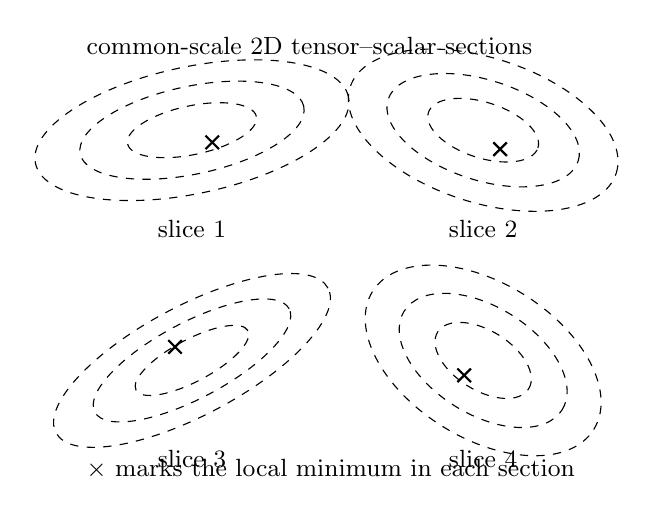
\begin{tikzpicture}[scale=0.86]
    \foreach \x/\y/\ang/\sx/\sy/\mx/\my/\lab in {
      -3.3/2.0/12/1.35/0.72/-3.0/1.82/{slice 1},
       1.0/2.0/-18/1.18/0.82/1.25/1.72/{slice 2},
      -3.3/-1.4/28/1.30/0.62/-3.55/-1.20/{slice 3},
       1.0/-1.4/-32/1.10/0.88/0.72/-1.62/{slice 4}}
    {
      \begin{scope}[shift={(\x,\y)},rotate=\ang]
        \draw[dashed] (0,0) ellipse ({1.75*\sx} and {1.30*\sy});
        \draw[dashed] (0,0) ellipse ({1.25*\sx} and {0.90*\sy});
        \draw[dashed] (0,0) ellipse ({0.72*\sx} and {0.50*\sy});
      \end{scope}
      \draw[thick] (\mx-0.10,\my-0.10) -- (\mx+0.10,\my+0.10);
      \draw[thick] (\mx-0.10,\my+0.10) -- (\mx+0.10,\my-0.10);
      \node[font=\small] at (\x,\y-1.45) {\lab};
    }
    \node[font=\small,anchor=west] at (-5.0,3.25) {common-scale 2D tensor--scalar sections};
    \node[font=\small,anchor=west] at (-5.0,-3.0) {$\times$ marks the local minimum in each section};
  \end{tikzpicture}
  \caption{Schematic four common-scale two-dimensional slices of a higher-dimensional tensor--scalar surrogate. The fixed tensor coordinates deform the local informational landscape; the cross marks the minimum in each slice.}
  \label{fig:nd-slices}
\end{figure}

% GENERATED LOCAL-BUILD FLAT PART - DO NOT MERGE
\chapter[Chiral--Fractal Temporal Topology]{Chiral--Fractal Temporal Topology as a Derived-Property Gate}
The Neutrinotime line motivates a fractal--chiral temporal topology as a comparison target. In the present derivation, the target is decomposed into independently testable quantities:
\[
I_{\rm top}[\Gamma],\qquad \chi[\Gamma],\qquad D_F[\Gamma].
\]
These denote, respectively, a topological invariant, a signed chirality/orientation observable, and a fractal-scaling observable of an orbit or invariant set \(\Gamma\).

A minimal chirality candidate is a signed holonomy,
\[
\chi[C]=\operatorname{sgn}\!\left(\oint_C A\right),
\]
whenever the dynamical state bundle supplies an admitted connection \(A\). Orientation reversal must reverse the sign of \(\chi\) while declared non-chiral invariants remain unchanged.

Fractality is measured prospectively from the derived tensor--scalar dynamics through \(D_F\), a renormalization relation, a Lyapunov diagnostic, or another explicit scaling test. A linear Kähler control supplies the non-fractal reference class.

The relation between event-localized NOW and a dynamical bifurcation locus remains an open bridge. They are maintained as separate typed objects until an equivalence theorem or prospective experiment closes that dependency.

\section{Visual intuition for chirality and event structure}
The schematic rendering in Figure~\ref{fig:temporal-ribbon-3d} shows a single trajectory lifted over an informational landscape, making visible the joint role of orbital phase and informational descent. Figure~\ref{fig:event-measure} then shows a schematic discrete event measure extracted from an evolving informational signal.
\begin{figure}[H]
  \centering
  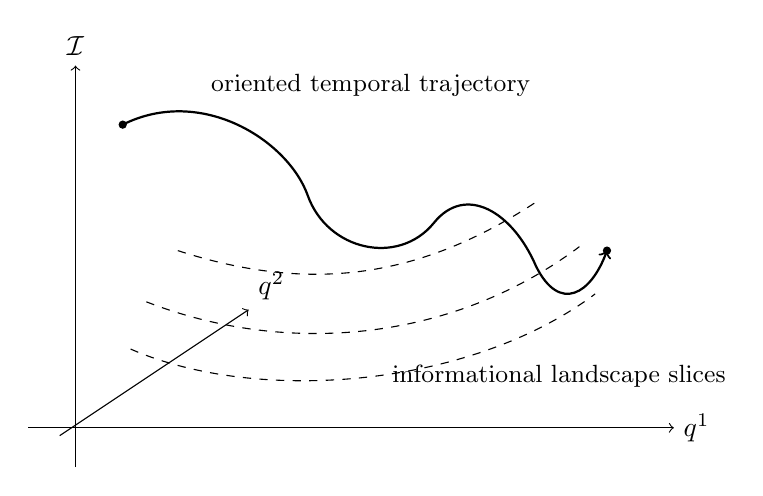
\begin{tikzpicture}[scale=1.0]
    \draw[->] (-4.0,-1.9) -- (4.2,-1.9) node[right] {$q^1$};
    \draw[->] (-3.4,-2.4) -- (-3.4,2.7) node[above] {$\mathcal I$};
    \draw[->] (-3.6,-2.0) -- (-1.2,-0.4) node[above right] {$q^2$};
    \draw[dashed] (-2.7,-0.9) .. controls (-1.1,-1.6) and (1.6,-1.4) .. (3.2,-0.2);
    \draw[dashed] (-2.5,-0.3) .. controls (-0.7,-1.0) and (1.4,-0.8) .. (3.0,0.4);
    \draw[dashed] (-2.1,0.35) .. controls (-0.4,-0.2) and (1.0,0.0) .. (2.5,1.0);
    \draw[->,thick]
      (-2.8,1.95)
      .. controls (-1.8,2.45) and (-0.7,1.75) .. (-0.45,1.05)
      .. controls (-0.20,0.35) and (0.70,0.15) .. (1.15,0.70)
      .. controls (1.55,1.20) and (2.15,0.85) .. (2.45,0.15)
      .. controls (2.75,-0.45) and (3.15,-0.20) .. (3.35,0.35);
    \fill (-2.8,1.95) circle (1.5pt);
    \fill (3.35,0.35) circle (1.5pt);
    \node[font=\small,anchor=west] at (-1.8,2.45) {oriented temporal trajectory};
    \node[font=\small,anchor=west] at (0.5,-1.25) {informational landscape slices};
  \end{tikzpicture}
  \caption{Schematic lifted slice of temporal evolution on the Kähler informational landscape. The vertical coordinate represents the informational functional $\mathcal{I}$ along an oriented trajectory.}
  \label{fig:temporal-ribbon-3d}
\end{figure}
\begin{figure}[H]
  \centering
  \begin{tikzpicture}[x=0.92cm,y=1.0cm]
    \draw[->] (0,0) -- (11.2,0) node[right] {$\lambda$};
    \draw[->] (0,-0.2) -- (0,3.0) node[above] {event weight};
    \draw[dashed] (0,1.0) -- (10.7,1.0) node[right,font=\small] {reference level};
    \foreach \x/\h in {0.7/0.35,1.5/0.75,2.4/0.45,3.2/1.55,4.0/0.65,5.1/2.35,6.0/0.55,6.9/1.25,7.8/0.50,8.9/1.90,9.8/0.70}
      \draw[thick] (\x,0) -- (\x,\h);
    \foreach \x/\h in {3.2/1.55,5.1/2.35,6.9/1.25,8.9/1.90}
      \fill (\x,\h) circle (1.8pt);
    \node[font=\small,anchor=west] at (3.35,2.65) {localized event support};
  \end{tikzpicture}
  \caption{Schematic discrete event measure on the ordering parameter. Selected localized peaks illustrate the event-support coordinate used to compare temporal evolution with NOW localization.}
  \label{fig:event-measure}
\end{figure}

% GENERATED LOCAL-BUILD FLAT PART - DO NOT MERGE
\chapter{Nature of the Temporal State}

The temporal architecture developed here begins with directed relational composability rather than an assumed temporal order. Realized relations form composable words. Their prefixes define distinct history occurrences, positive transition activity supplies an intrinsic duration weight, and the combination produces temporal precedence. NOW is then the maximal supported frontier of the realized occurrence history. A downstream half-frame construction provides a finite-support realization in which neighboring temporal frames overlap while preserving the total intrinsic elapsed measure.

\section{Pretime relational composition}

Let
\[
\mathcal G=(S,E,s,t)
\]
be a directed relational multigraph. An edge $e:a\to b$ carries source and target labels. Two relations compose when
\[
\boxed{t(e_k)=s(e_{k+1}).}
\]
A finite realized word is
\[
\boxed{
P_n=e_n\circ\cdots\circ e_1,
}
\]
with prefixes
\[
P_0=\mathrm{id},
\qquad
P_k=e_k\circ\cdots\circ e_1.
\]
Define the realized occurrence
\[
\boxed{\nu_k=(P_k,x_k),}
\]
where $x_k$ is the terminal state label of $P_k$. Repeated state labels remain distinct occurrences because the full prefixes differ.

Define the prefix relation
\[
\boxed{
\nu_i\sqsubseteq\nu_j
\iff
\exists Q:\ P_j=Q\circ P_i.
}
\]
On prefix-labelled occurrences it is reflexive, transitive and antisymmetric. Along one realized serial word it is total.

\section{Transition traffic and intrinsic duration}

For an admitted active pair,
\[
W_+=Me^{A/2},
\qquad
W_-=Me^{-A/2},
\qquad M>0,
\]
and therefore
\[
\boxed{\mathfrak a=W_++W_-=2M\cosh(A/2)>0,}
\]
\[
\boxed{\mathfrak j=W_+-W_-=2M\sinh(A/2).}
\]
Independent-channel extensivity, continuity and invariance of duration under orientation exchange force the local duration density to have the form
\[
F(W_+,W_-)=C(W_++W_-),
\qquad C>0.
\]
In intrinsic activity units $C=1$.

For any increasing local edge parameter $\lambda_e$,
\[
\boxed{
\theta(e)=\int_e\mathfrak a\,d\lambda_e>0
}
\]
is invariant under admitted reparameterization. The infinitesimal form is
\[
\boxed{d\Theta=\mathfrak a\,d\lambda_e.}
\]
For a realized prefix,
\[
\boxed{
\Theta(P_k)=\sum_{r=1}^{k}\theta(e_r).
}
\]
Hence a strict prefix extension obeys
\[
\boxed{
\nu_i\sqsubset\nu_j
\Longrightarrow
\Theta(P_i)<\Theta(P_j).
}
\]
On one serial word the converse holds. Temporal precedence is therefore defined on realized occurrences by
\[
\boxed{
\nu_i\prec_T\nu_j
\iff
\nu_i\sqsubset\nu_j,
}
\]
with $\Theta$ providing its strictly increasing scalar realization.

\section{Recurrence and temporal advance}

A relational cycle in state labels,
\[
A\to B\to A,
\]
produces
\[
(A,P_0)\prec_T(B,P_1)\prec_T(A,P_2).
\]
Thus the state label can recur while the realized occurrence history continues to advance. The distinction between state identity and occurrence identity is retained by the full relation prefix.

\section{Duration and orientation}

The normalized directional coordinate is
\[
\boxed{
\chi=\frac{\mathfrak j}{\mathfrak a}=\tanh(A/2).
}
\]
Using the Shannon affinity in bits,
\[
A=(\ln2)\sigma,
\]
we obtain
\[
\boxed{
\chi=\tanh\!\left(\frac{\ln2}{2}\sigma\right)
}
\]
and
\[
\boxed{
d\Theta=2M\cosh\!\left(\frac{\ln2}{2}\sigma\right)d\lambda_e.}
\]
Under orientation reversal $A\mapsto-A$, duration is even and $\chi$ is odd. At $A=0$,
\[
\boxed{\theta(e)>0,\qquad \chi=0.}
\]
The accumulated duration coordinate and the local directional-affinity coordinate are therefore distinct.

With
\[
M_{ab}
=\frac{\sqrt{\rho_R(a)\rho_R(b)}}{\tfrac12[\eta_R(a)+\eta_R(b)]},
\]
the intrinsic duration density becomes
\[
\boxed{
\frac{d\Theta}{d\lambda_e}
=
2\frac{\sqrt{\rho_R(a)\rho_R(b)}}{\tfrac12[\eta_R(a)+\eta_R(b)]}
\cosh\!\left(\frac{\ln2}{2}\sigma_{ab}\right).
}
\]

\section{Half-frame temporal gluing}

Let a finite serial sector contain $N$ discrete temporal frames. Associate the phase budget
\[
\boxed{\Phi_N=2\pi N.}
\]
Each frame is split into two half-supports,
\[
\boxed{
|n\rangle
\mapsto
\frac{|n,L\rangle+|n,R\rangle}{\sqrt2}.
}
\]
Neighboring halves are identified by
\[
\boxed{|n,R\rangle\sim|n+1,L\rangle.}
\]
The resulting support sequence has $N+1$ elements,
\[
\boxed{
|1|,\ |12|,\ |23|,\ldots,\ |N-1,N|,\ |N|.
}
\]
The first modular sectors therefore read
\[
\begin{aligned}
2\pi &: \quad |1|1|,\\
4\pi &: \quad |1|12|2|,\\
6\pi &: \quad |1|12|23|3|,\\
8\pi &: \quad |1|12|23|34|4|.
\end{aligned}
\]
The counting identity is
\[
\boxed{2N-(N-1)=N+1.}
\]

For frame amplitudes $a_n$, the neighboring overlap and antisymmetric seam amplitudes are
\[
\boxed{
b_n=\frac{a_n+a_{n+1}}2,
\qquad
d_n=\frac{a_n-a_{n+1}}2.
}
\]
Together with the two boundary amplitudes they satisfy the exact norm decomposition
\[
\boxed{
\sum_{j=0}^{N}|b_j|^2
+\sum_{n=1}^{N-1}|d_n|^2
=\sum_{n=1}^{N}|a_n|^2.
}
\]
Equal neighboring phase therefore occupies the overlap support, while opposite neighboring phase produces an interface null and transfers weight into the seam-defect sector.

The same topology acts on the positive activity-derived elapsed measure. For frame intervals $\theta_n>0$, define
\[
\boxed{\ell_0=\frac{\theta_1}{2},}
\]
\[
\boxed{\ell_n=\frac{\theta_n+\theta_{n+1}}2,
\qquad 1\le n<N,}
\]
and
\[
\boxed{\ell_N=\frac{\theta_N}{2}.}
\]
Then
\[
\boxed{
\sum_{j=0}^{N}\ell_j
=\sum_{n=1}^{N}\theta_n
=\Theta_N.
}
\]
Thus neighboring overlap redistributes temporal support while preserving the total intrinsic elapsed measure exactly.

\section{Half-frame path complex and long-wave topology}

The $N+1$ glued supports form vertices $v_0,\ldots,v_N$. Each full temporal frame becomes one oriented edge
\[
\boxed{e_n=[v_{n-1},v_n].}
\]
Hence the half-frame quotient generates the path complex $P_{N+1}$. Its incidence operator is
\[
\boxed{\partial_1 e_n=v_n-v_{n-1}.}
\]
For positive frame weights $w_n$, the support Laplacian is
\[
\boxed{
L_V=D_N\operatorname{diag}(w_n)D_N^T,
}
\]
with
\[
L_V=L_V^T,
\qquad
L_V\succeq0,
\qquad
L_V\mathbf1=0.
\]
For uniform $w_n=w$, its exact spectrum is
\[
\boxed{
\lambda_k
=2w\left[1-\cos\left(\frac{k\pi}{N+1}\right)\right],
\qquad k=0,\ldots,N.
}
\]
The low sector approaches
\[
\boxed{
\lambda_k
=w\left(\frac{k\pi}{N+1}\right)^2
+O\!\left(\frac{k^4}{(N+1)^4}\right).
}
\]
This provides the topological origin of the local path incidence used by the discrete Temporal Wave coarse-graining sector.

\section{NOW as the maximal realized frontier}

For an admitted transition edge define the gauge-invariant event signature
\[
\boxed{
q_e=
\sqrt{
 d_{FS}(a,b)^2+
 \kappa^2\Delta H_e^2+
 \kappa^2\sigma_e^2
 }\ge0.
}
\]
The nonzero event carrier is
\[
\mathcal E_q
=\operatorname{supp}_{\rm at}
\left(\sum_e q_e\delta_{s_e}\right).
\]
For a finite realized down-set $D$ of occurrence prefixes, define
\[
D_q=\{\nu\in D:q_{e(\nu)}>0\}.
\]
Then
\[
\boxed{
\mathcal N(D)
=\operatorname{Max}_{\prec_T}(D_q).
}
\]
For a serial history the frontier contains the latest supported occurrence. For independent concurrent branches it is the antichain of maximal supported occurrences.

The half-frame path gives a concrete serial realization of the same rule. At stage $N$ the terminal pure support is
\[
\boxed{\mathrm{NOW}_N\leftrightarrow|N|_\partial.}
\]
When frame $N+1$ is realized,
\[
\boxed{
|N|_\partial
\longmapsto
|N,N+1|,
\qquad
\mathrm{NOW}_{N+1}\leftrightarrow|N+1|_\partial.
}
\]
The previous boundary is thereby incorporated into the neighboring-history interface while the newly created right boundary becomes the maximal serial support.

At the level of elapsed measure, if the new frame carries $\theta_{N+1}>0$, the support extension increases the total measure by exactly
\[
\boxed{\Delta\Theta=\theta_{N+1}.}
\]
Thus the half-frame moving frontier and the prefix-extension ordering share the same positive one-step temporal increment.

\section{Relative clocks and calibrated elapsed time}

For two active subsystems on a common relational comparison patch,
\[
\boxed{
N_R(x|r)
=\frac{d\Theta_x}{d\Theta_r}
=\frac{\mathfrak a_x}{\mathfrak a_r}>0.
}
\]
Reference changes compose multiplicatively,
\[
N_{x|s}=N_{x|r}N_{r|s}.
\]
A physical reference-clock calibration supplies the conversion scale,
\[
\boxed{dt=T_r\,d\Theta_r,}
\]
and therefore
\[
\boxed{d\hat\tau_x=N_Rdt.}
\]
On the admitted lapse/phase-rate bridge,
\[
\boxed{r_t=N_Rr_n^{(\tau)}.}
\]

\section{Phase topology, bifurcation and transport}

The information--phase link is
\[
L_e
=G_e\exp\!\left[i\kappa(\Delta H_e+\sigma_e)\right],
\qquad
\boxed{\kappa=\frac{\ln2}{24\pi}}.
\]
On a closed cycle,
\[
\boxed{
\operatorname{Arg}\prod_{e\in C}L_e
=\gamma_B(C)+\kappa\sum_{e\in C}\sigma_e
\pmod{2\pi}.
}
\]
At a supported maximal event occurrence the state update is represented by
\[
\boxed{
\Psi_T(s_n^+)=B_n\Psi_T(s_n^-).
}
\]
Between event occurrences,
\[
\boxed{\Psi_{n+1}=U_n\Psi_n.}
\]
A realized operator word has the compositional form
\[
\boxed{
\Psi_N
=U_{N-1}B_{N-1}\cdots U_2B_2U_1B_1\Psi_0.
}
\]
The operator composition and the relational occurrence prefix carry the same realized lineage order.

Within the Zeta--Collatz Temporal Wave candidate, a Hermitian frame Hamiltonian acts on the already-derived intrinsic coordinate,
\[
\boxed{
i\partial_\Theta a(\Theta)=H_{\zeta C}a(\Theta).
}
\]
The half-frame quotient then supplies the topology-driven interface readout. In the declared five-frame reference witness, a sharp initial frame has raw neighboring-interface occupancy $F_{1/2}(0)=0.25$, while the evolved state at the declared intrinsic interval reaches an occupancy above $0.5$. This is retained as a finite reference witness of dynamical frame-to-interface spreading; general dynamical classification remains subject to its separate gate.

\section{Memory and retrodiction}

Memory retains the realized occurrence lineage together with its temporal carriers. ORCHORBITAL records the active-attractor sequence
\[
\alpha=(a_1,\ldots,a_N),
\]
signed winding
\[
\mathcal W=(\Delta W_1,\ldots,\Delta W_N),
\]
and residence-bound radial lineage
\[
\mathcal R=(\rho_1,\ldots,\rho_N).
\]
Retrodiction reconstructs hidden histories on these retained strata. Spatial Offset Divergence audits collision fibres of compressed observation maps, while the cumulative coordinate $\Theta(P_k)$ supplies the intrinsic duration carried by the same realized prefix history.

\section{Derived temporal architecture}

The present derivation is
\[
\boxed{
\begin{aligned}
&\text{DIRECTED RELATIONAL COMPOSABILITY}\\
&\downarrow\\
&\text{REALIZED WORDS AND PREFIX OCCURRENCES}\\
&\downarrow\\
&\mathfrak a=W_++W_-,\quad \mathfrak j=W_+-W_-\\
&\downarrow\\
&\theta(e)=\int_e\mathfrak a\,d\lambda_e,\quad
\Theta(P)=\sum_e\theta(e),\quad
\chi=\mathfrak j/\mathfrak a\\
&\downarrow\\
&\text{TEMPORAL PRECEDENCE FROM PREFIX EXTENSION}\\
&\downarrow\\
&\text{TEMPORAL WAVE / HALF-FRAME OVERLAP SUPPORT}\\
&\downarrow\\
&\text{NOW}=\operatorname{Max}(\text{SUPPORTED REALIZED OCCURRENCES})\\
&\downarrow\\
&\text{BIFURCATION}\to\text{TRANSPORT}\to\text{MEMORY}\to\text{RETRODICTION}.
\end{aligned}
}
\]
Physical clock calibration, spin-$1/2$/four-$\pi$ binding and downstream spacetime closure retain their declared evidence gates.

% GENERATED LOCAL-BUILD FLAT PART - DO NOT MERGE
\chapter{Wave Structure of Time}

The relational transition layer carries a unit-modulus phase link $L_{ab}\in U(1)$ and a positive symmetric mobility $M_{ab}$.  For an oriented edge $e:a\to b$, define the covariant difference
\[
(D_L\Phi)_{ab}=\Phi_b-L_{ab}\Phi_a.
\]
The associated positive quadratic form is
\[
\mathcal E_W[\Phi]
=\sum_e M_e |(D_L\Phi)_e|^2,
\]
which defines the Hermitian positive-semidefinite Temporal Wave operator
\[
\boxed{
K_M=D_L^\dagger\operatorname{diag}(M_e)D_L.
}
\]
The mobility is inherited from the relational kinetic pair,
\[
M_{ab}
=\frac{\sqrt{\rho_R(a)\rho_R(b)}}{\tfrac12[\eta_R(a)+\eta_R(b)]}.
\]
Thus the wave stiffness uses the same positive coefficient that controls the symmetric transition rate at zero antisymmetric drive.

\section{Relational viscosity and damping}

Let
\[
\bar\eta_{ab}=\frac{\eta_R(a)+\eta_R(b)}2.
\]
The viscosity-weighted covariant operator is
\[
\boxed{
C_\eta
=D_L^\dagger\operatorname{diag}(\bar\eta_e)D_L.
}
\]
For conjugate wave coordinates $(q,p)$, the tested candidate evolution is
\[
\dot q=-p,
\qquad
\dot p=K_Mq-C_\eta p,
\]
or equivalently
\[
\boxed{
\ddot q+C_\eta\dot q+K_Mq=0.
}
\]
With
\[
\mathcal H_T
=\frac12p^\dagger p+\frac12q^\dagger K_Mq,
\]
the exact balance is
\[
\boxed{
\frac{d\mathcal H_T}{d\lambda}
=-p^\dagger C_\eta p\le0.
}
\]

\section{Heterogeneous long-wave limit}

For a one-dimensional periodic heterogeneous relational cell, let $M_e$ and $\eta_e$ denote the edge mobility and pair viscosity.  The acoustic cell corrector yields
\[
\boxed{
M_{\rm eff}
=\left\langle M_e^{-1}\right\rangle^{-1}
}
\]
and
\[
\boxed{
\beta_{\rm eff}
=M_{\rm eff}^2
\left\langle\frac{\eta_e}{M_e^2}\right\rangle.
}
\]
The long-wave positive-frequency branch is therefore
\[
\boxed{
\omega(k)
=\sqrt{M_{\rm eff}}\,|k|
-i\frac{\beta_{\rm eff}}2k^2
+O(|k|^3).
}
\]
For uniform relational fields,
\[
M_{\rm eff}=\frac{\rho_0}{\eta_0},
\qquad
\beta_{\rm eff}=\eta_0.
\]

\section{Holonomy shift}

For total closed-cell phase $\phi$ and Bloch phase $\theta$, the tested heterogeneous branch depends on the shifted wave number
\[
\boxed{
k_{\rm eff}=\frac{\operatorname{wrap}(\theta-\phi)}{L}.
}
\]
Hence
\[
\boxed{
\omega
=\sqrt{M_{\rm eff}}\,|k_{\rm eff}|
-i\frac{\beta_{\rm eff}}2k_{\rm eff}^2+\cdots.
}
\]
On a uniform $N$-cycle the exact spectrum is
\[
\lambda_m
=4MN^2
\sin^2\!\left(\frac{2\pi m-\phi}{2N}\right),
\]
so a nontrivial principal holonomy opens a positive lowest-mode gap.

These results provide the upstream wave carrier consumed by the NOW localization layer.  Metric-clock calibration remains assigned to the later Einstein-closure stage of the dependency graph.

% GENERATED LOCAL-BUILD FLAT PART - DO NOT MERGE
\chapter{NOW as a Positive Wave-Active Transition Support}

The NOW layer separates structural event signature, kinetic pace, directional current and dynamical wave activation.

\section{Structural transition signature}

For an admitted transition edge $e:a\to b$, define
\[
\boxed{
q_e=
\sqrt{
 d_{FS}(a,b)^2
 +\kappa^2\Delta H_e^2
 +\kappa^2\sigma_e^2
}\ge0.
}
\]
The structural atomic event measure is
\[
\mathcal K_T^+
=\sum_e q_e\,\delta_{s_e},
\]
with carrier
\[
\boxed{
\mathcal N_{\rm sig}
=\operatorname{supp}_{\rm at}\mathcal K_T^+.
}
\]
The Fubini--Study distance and the scalar information increments make $q_e$ invariant under local state-phase choices.

\section{Activity and directed current}

The positive directed kinetic pair is
\[
W_{a\to b}=M_{ab}e^{A_{ab}/2},
\qquad
W_{b\to a}=M_{ab}e^{-A_{ab}/2}.
\]
Its symmetric and antisymmetric combinations are
\[
\boxed{
\mathfrak a_{ab}=2M_{ab}\cosh(A_{ab}/2)>0,
}
\]
\[
\boxed{
\mathfrak j_{ab}=2M_{ab}\sinh(A_{ab}/2).
}
\]
They obey the exact invariant
\[
\boxed{
\mathfrak a_{ab}^2-\mathfrak j_{ab}^2=4M_{ab}^2,
}
\]
so the mobility entering the Temporal Wave operator is reconstructed as
\[
\boxed{
M_{ab}
=\frac12\sqrt{\mathfrak a_{ab}^2-\mathfrak j_{ab}^2}.
}
\]

\section{Temporal Wave activation}

Let $\Phi$ denote the node amplitude of the Temporal Wave and
\[
(D_L\Phi)_e=\Phi_b-L_{ab}\Phi_a.
\]
The local wave activation is
\[
\boxed{
\epsilon_e^{(W)}
=M_e|(D_L\Phi)_e|^2\ge0.
}
\]
It is invariant under the simultaneous local phase transformation of $\Phi$ and $L$.  A covariantly parallel edge has zero activation.

The total activation is exactly the Temporal Wave quadratic form,
\[
\boxed{
\sum_e\epsilon_e^{(W)}
=\Phi^\dagger K_M\Phi.
}
\]
For the tested nontrivial-holonomy ring, the positive spectral gap therefore supplies a positive total activation for every nonzero wave state.

\section{Wave-active realization of NOW}

Structural event signature and wave activation combine through the positive atomic measure
\[
\boxed{
\mathcal R_{\rm NOW}^{(W)}
=\sum_e q_e\epsilon_e^{(W)}\,\delta_{s_e}.
}
\]
Its support is
\[
\boxed{
\mathcal N_W
=\operatorname{supp}_{\rm at}\mathcal R_{\rm NOW}^{(W)}
=\mathcal N_{\rm sig}
\cap
\operatorname{supp}\{e:\epsilon_e^{(W)}>0\}.
}
\]
The equality follows directly from positivity of both factors.  The structural carrier $\mathcal N_{\rm sig}$ preserves transition typing and lineage; $\mathcal N_W$ carries the tested dynamical realization candidate passed to the bifurcation layer.

\section{Pushforward support}

For any positive atomic measure
\[
\mu=\sum_j a_j\delta_{x_j},
\qquad a_j>0,
\]
and any map $f$ on its support,
\[
(f_*\mu)(\{y\})
=\sum_{j:f(x_j)=y}a_j.
\]
Every image atom retains positive mass, giving
\[
\boxed{
\operatorname{supp}_{\rm at}(f_*\mu)
=f(\operatorname{supp}_{\rm at}\mu).
}
\]
This applies both to the structural positive measure and to the wave-active realization measure.

The resulting NOW boundary therefore carries four typed observables: structural signature $q_e$, symmetric activity $\mathfrak a_e$, directed current $\mathfrak j_e$, and wave activation $\epsilon_e^{(W)}$.  Their next decomposition supplies the wave-magnitude and bifurcation-orientation coordinates.

% GENERATED LOCAL-BUILD FLAT PART - DO NOT MERGE
\chapter{Causal Bifurcation}

The wave-active NOW carrier localizes the events on which the bifurcation operator acts.  For a realized event $s_e\in\mathcal N_W$,
\[
\Psi_T(s_e^+)=B_e\Psi_T(s_e^-).
\]

\section{Hyperbolic kinetic coordinates}

At the NOW boundary the activity/current pair obeys
\[
\mathfrak a=2M\cosh(A/2),
\qquad
\mathfrak j=2M\sinh(A/2).
\]
The invariant coordinate is
\[
\boxed{
M=\frac12\sqrt{\mathfrak a^2-\mathfrak j^2},
}
\]
and the oriented coordinate is
\[
A=2\operatorname{artanh}\!\left(\frac{\mathfrak j}{\mathfrak a}\right).
\]
Using
\[
\kappa=\frac{\ln2}{24\pi},
\qquad
\beta=\frac{\kappa A}{\ln2},
\]
gives
\[
\boxed{
\beta=\frac{1}{12\pi}
\operatorname{artanh}\!\left(\frac{\mathfrak j}{\mathfrak a}\right),
\qquad
A=24\pi\beta.
}
\]
Thus
\[
\boxed{
\mathfrak a=2M\cosh(12\pi\beta),
\qquad
\mathfrak j=2M\sinh(12\pi\beta).
}
\]
The coordinate $M$ feeds the Temporal Wave stiffness and the coordinate $\beta$ feeds the directional bifurcation phase.

\section{Wave-active event gate}

The NOW realization weight is
\[
r_e^{(W)}=q_e\epsilon_e^{(W)}\ge0.
\]
For a declared Hermitian generator $G$, define the directional unitary family
\[
B_\phi(\beta_e)=e^{-i\beta_eG}.
\]
The tested gate is
\[
\boxed{
r_e^{(W)}>0\Rightarrow B_e=B_\phi(\beta_e),}
\]
\[
\boxed{
r_e^{(W)}=0\Rightarrow B_e=I.}
\]
The positive product $q_e\epsilon_e^{(W)}$ therefore controls event admission, while the sign and magnitude of $\beta_e$ control the orientation of the realized unitary action.

Under current reversal,
\[
\mathfrak j\mapsto-\mathfrak j,
\]
we have
\[
M\mapsto M,
\qquad
\beta\mapsto-\beta,
\]
and hence
\[
\boxed{
B_\phi(-\beta)=B_\phi(\beta)^\dagger.
}
\]
The same reversal preserves the Temporal Wave stiffness channel and inverts the directional bifurcation action.

\section{General representation and polar branch}

For an additive scalar event parameter $q$, representation consistency gives
\[
B(0)=I,
\qquad
B(q_1+q_2)=B(q_2)B(q_1),
\]
with strongly continuous invertible family
\[
B(q)=e^{qG}.
\]
A unitary family uses a self-adjoint generator $A$,
\[
B(q)=e^{-iqA}.
\]

The implemented polar reference branch also admits a positive semidefinite dissipator $D$,
\[
C(q)=e^{-qD},
\qquad
U(\beta)=e^{-i\beta G},
\]
and the ordered polar event operator
\[
\boxed{
B_{\rm polar}=C(q)U(\beta).
}
\]
The wave-active gate fixes the event support and directional phase coordinate.  The contractive-strength calibration and physical generator selection remain downstream evidence targets within the bifurcation program.

The resulting bifurcation output is passed in ordered form to the Temporal Transport layer.

% GENERATED LOCAL-BUILD FLAT PART - DO NOT MERGE
\chapter{Temporal Transport and Internal Elapsed Activity}

Temporal Transport composes smooth Temporal Wave evolution with the localized bifurcation events supplied by the wave-active NOW carrier.

\section{Smooth Temporal Wave segment}

Let
\[
K=K_M\succeq0,
\qquad
C=C_\eta\succeq0,
\]
and use the phase-space state
\[
x=\begin{pmatrix}q\\p\end{pmatrix}.
\]
The smooth generator is
\[
\boxed{
A_W=
\begin{pmatrix}
0&-I\\
K&-C
\end{pmatrix}.
}
\]
The wave energy has metric
\[
\boxed{
Q_W=
\begin{pmatrix}
K&0\\
0&I
\end{pmatrix},
}
\]
with
\[
\mathcal H_T=\frac12x^\dagger Q_Wx.
\]
A direct calculation gives
\[
\boxed{
A_W^\dagger Q_W+Q_WA_W
=
\begin{pmatrix}
0&0\\
0&-2C
\end{pmatrix}\preceq0.
}
\]

For an ordered increment $h>0$, the reference smooth segment is the Cayley transform
\[
\boxed{
U_h^{(W)}
=\left(I-\frac h2A_W\right)^{-1}
\left(I+\frac h2A_W\right).
}
\]
It obeys the exact discrete energy inequality
\[
\boxed{
(U_h^{(W)})^\dagger Q_WU_h^{(W)}\preceq Q_W.
}
\]
For $C=0$ the inequality becomes equality, giving a $Q_W$-unitary conservative segment.

\section{Interrupted transport}

For smooth segments $U_n$ and localized event operators $B_n$, chronological transport is
\[
\boxed{
\mathcal U_{f\leftarrow i}
=U_NB_NU_{N-1}B_{N-1}\cdots U_1B_1U_0.
}
\]
The multiplication order is inherited from the ordered event sequence.

A sufficient energy-compatible event condition is
\[
[G_n,Q_W]=0
\]
for the Hermitian directional generator $G_n$.  Then
\[
B_n=e^{-i\beta_nG_n}
\]
satisfies
\[
B_n^\dagger Q_WB_n=Q_W.
\]
For one shared wave-energy metric, a product of $Q_W$-contractive smooth segments and $Q_W$-unitary realized events obeys
\[
\boxed{
\mathcal U_{f\leftarrow i}^\dagger
Q_W
\mathcal U_{f\leftarrow i}
\preceq Q_W.
}
\]
The generic interrupted-product contract also retains its spectral-norm bound, exact cut identity and conditioning audit.

\section{Internal elapsed activity}

The positive activity layer defines an internal elapsed coordinate before metric-clock calibration. Let $\lambda$ be an admissible increasing ordering parameter, let $\mathfrak a(\lambda)>0$ denote realized temporal activity, and let $\mathfrak a_\star>0$ be a declared system-internal reference activity. Define
\[
\boxed{
d\tau_{\rm int}
=\frac{\mathfrak a(\lambda)}{\mathfrak a_\star}\,d\lambda.
}
\]
For a discrete ordered path,
\[
\boxed{
\tau_{{\rm int},N}
=\sum_{n=0}^{N-1}
\frac{\mathfrak a_n}{\mathfrak a_\star}\,\Delta\lambda_n,
\qquad
\Delta\lambda_n>0.
}
\]
Every admitted increment is strictly positive, so the internal elapsed coordinate is strictly monotone along the realized ordered path.

\section{Reparameterization covariance}

For an increasing relabeling $\lambda'=f(\lambda)$, let activity transform as a one-density,
\[
\mathfrak a'(\lambda')
=\mathfrak a(\lambda)\frac{d\lambda}{d\lambda'}.
\]
Then
\[
\mathfrak a'(\lambda')\,d\lambda'
=\mathfrak a(\lambda)\,d\lambda,
\]
and hence
\[
\boxed{d\tau'_{\rm int}=d\tau_{\rm int}.}
\]

\section{Relational density, viscosity and internal pace}

Using
\[
\mathfrak a_{ab}
=2M_{ab}\cosh(A_{ab}/2),
\]
with
\[
M_{ab}
=\frac{\sqrt{\rho_R(a)\rho_R(b)}}{\tfrac12[\eta_R(a)+\eta_R(b)]},
\]
gives
\[
\boxed{
\frac{d\tau_{\rm int}}{d\lambda}
=\frac{2}{\mathfrak a_\star}
\frac{\sqrt{\rho_R(a)\rho_R(b)}}{\tfrac12[\eta_R(a)+\eta_R(b)]}
\cosh(A_{ab}/2).
}
\]
Within this candidate, relational density raises the internal activity pace and relational viscosity lowers it. Reversing the antisymmetric drive leaves the pace invariant while the directed current reverses sign.

The resulting transport layer therefore carries both an ordered state propagator and the system-internal elapsed-activity coordinate consumed by the Memory node.

\part{Memory and Reconstruction}
% GENERATED LOCAL-BUILD FLAT PART - DO NOT MERGE
\chapter{Memory and Retrodiction}

The memory layer is developed downstream of Temporal Transport. The current executable branch combines an event-imprinted memory coordinate with a Kepler--Newton evolution law parameterized by the internal elapsed activity variable.

\section{Oriented memory coordinate}

Assign a complex memory coordinate
\[
m(s)=x_M(s)+iy_M(s)=r_M(s)e^{i\theta_M(s)}.
\]
The oriented edge functional is
\[
\boxed{
A^{(M)}_{ab}
=\lambda_M\operatorname{Im}[m(a)^*m(b)]
=\lambda_M r_a r_b\sin(\theta_b-\theta_a).
}
\]
For a closed polygonal orbit,
\[
\sum_C A^{(M)}_e
=2\lambda_M\mathcal A_M(C),
\]
where \(\mathcal A_M(C)\) is the signed enclosed area.

\section{Event-imprinted memory coordinate}

For the states immediately before and after an admitted event, define
\[
R_n^\pm=\Psi_n^\pm(\Psi_n^\pm)^\dagger,
\qquad
\bar\rho_n^\pm=\frac{R_n^\pm}{\operatorname{tr}R_n^\pm}.
\]
The projective memory imprint is
\[
\boxed{\Delta M_n=\bar\rho_n^+-\bar\rho_n^-}.
\]
With declared Hermitian memory observables \(Q_M,P_M\),
\[
m=\operatorname{tr}(\rho Q_M)+i\operatorname{tr}(\rho P_M),
\]
and the event displacement in the memory plane is
\[
\boxed{
\delta m_n
=\operatorname{tr}(\Delta M_nQ_M)
+i\operatorname{tr}(\Delta M_nP_M).
}
\]
Independent global phase changes of the pre/post states leave this projective imprint invariant.

\section{CP1 K\"ahler-derived memory frame}

The broad Hermitian-observable projection remains the general family. For the pure-qubit \(\mathbb{CP}^1\) reference subclass, the local memory frame is built from the standard Fubini--Study geometry of quantum-state space \cite{ProvostVallee1980}; the IDT-specific content is its use as a typed memory carrier and reconstruction frame.

Let \(\mathbf n_a,\mathbf n_b\in S^2\) be the Bloch vectors of two non-antipodal pure states and
\[
\theta_{ab}=\arccos(\mathbf n_a\cdot\mathbf n_b).
\]
Then
\[
d_{FS}(a,b)=\frac{\theta_{ab}}{2}
\]
and the half-angle tangent logarithm at \(a\) is
\[
\boxed{
\xi^{FS}_{a\to b}
=\frac12\frac{\theta_{ab}}{\sin\theta_{ab}}
\left(\mathbf n_b-\cos\theta_{ab}\,\mathbf n_a\right),
\qquad
\|\xi^{FS}_{a\to b}\|=d_{FS}(a,b).
}
\]
For the first admitted nonzero local displacement define
\[
\mathbf e_Q=\frac{\xi^{FS}}{\|\xi^{FS}\|},
\qquad
\boxed{\mathbf e_P=\mathbf n\times\mathbf e_Q}.
\]
The resulting K\"ahler-conjugate tangent dyad gives
\[
\boxed{
\delta m
=\xi^{FS}\cdot\mathbf e_Q
+i\,\xi^{FS}\cdot\mathbf e_P,
\qquad
|\delta m|=d_{FS}.
}
\]
Between non-antipodal anchors, let \(R_{b\leftarrow a}\in SO(3)\) be the minimal rotation along the selected Bloch great-circle geodesic. The frame propagates by
\[
\boxed{
\mathbf e_Q^{(b)}=R_{b\leftarrow a}\mathbf e_Q^{(a)},
\qquad
\mathbf e_P^{(b)}=R_{b\leftarrow a}\mathbf e_P^{(a)}.
}
\]
This preserves tangency, orthonormality and orientation,
\[
\mathbf e_P^{(b)}=\mathbf n_b\times\mathbf e_Q^{(b)}.
\]
In the \(\mathbb{CP}^1\) reference subclass this is the discrete Levi--Civita/K\"ahler parallel transport along the selected geodesic. Antipodal points are treated as a geodesic ambiguity and fail closed.

\section{Internal-time Newton dynamics}

The internal evolution increment inherited from temporal activity is
\[
d\tau_{\rm int}=\frac{\mathfrak a}{\mathfrak a_\star}\,d\lambda.
\]
On the memory plane we introduce the effective central parameter \(\mu_M>0\) and
\[
V_M(r_M)=-\frac{\mu_M}{r_M}.
\]
The smooth memory trajectory obeys
\[
\boxed{
\frac{d^2m}{d\tau_{\rm int}^2}
=-\mu_M\frac{m}{|m|^3}.
}
\]

\section{Kepler structure}

Define
\[
\varepsilon_M
=\frac12\left|\frac{dm}{d\tau_{\rm int}}\right|^2
-\frac{\mu_M}{r_M},
\qquad
h_M
=\operatorname{Im}\!\left[m^*\frac{dm}{d\tau_{\rm int}}\right].
\]
The central-force law gives the areal relation
\[
\boxed{
\frac{d\mathcal A_M}{d\tau_{\rm int}}
=\frac{h_M}{2}.
}
\]
The corresponding conic is
\[
r_M(\nu)
=\frac{p_M}{1+e_M\cos\nu},
\qquad
p_M=\frac{h_M^2}{\mu_M}.
\]
For a bound nondegenerate orbit,
\[
a_M=-\frac{\mu_M}{2\varepsilon_M},
\qquad
T_M^2=\frac{4\pi^2}{\mu_M}a_M^3.
\]
Combining the areal law with the earlier memory circulation yields
\[
\boxed{
\frac{d}{d\tau_{\rm int}}
\left(\sum_C A_e^{(M)}\right)
=\lambda_M h_M.
}
\]

\section{Event action and orbital bifurcation}

The NOW layer supplies a non-negative gauge-invariant event magnitude \(q_n\). Using that amplitude and the projected event imprint, define the normalized localized memory action
\[
\boxed{
S_n^{(M)}(m)
=q_n\operatorname{Re}(\delta m_n^*m).
}
\]
The event-augmented memory Lagrangian is
\[
L_M
=\frac12|\dot m|^2+\frac{\mu_M}{|m|}
+\sum_n\delta(\tau_{\rm int}-\tau_n)S_n^{(M)}(m).
\]
Integrating the Euler--Lagrange equation through one event gives
\[
\boxed{
\Delta v_{M,n}=q_n\delta m_n,
\qquad
v_{M,n}^+=v_{M,n}^-+q_n\delta m_n.
}
\]
At fixed event position the orbital invariants change by
\[
\boxed{
\Delta E_M
=q_n\operatorname{Re}(v_M^*\delta m_n)
+\frac12q_n^2|\delta m_n|^2,
}
\]
\[
\boxed{
\Delta h_M=q_n\operatorname{Im}(m^*\delta m_n).
}
\]
The post-event pair \((E_M^+,h_M^+)\) determines the next smooth Kepler-class orbit.

\section{Identifying the central memory parameter}

Within the Kepler reference class, \(\mu_M\) can be inferred from the orbit itself. From
\[
p_M=\frac{h_M^2}{\mu_M}
\]
one obtains
\[
\boxed{\mu_M=\frac{h_M^2}{p_M}}.
\]
For a bound ellipse with periapsis \(r_p\) and apoapsis \(r_a\),
\[
a_M=\frac{r_p+r_a}{2},
\qquad
p_M=\frac{2r_pr_a}{r_p+r_a}.
\]
The third law gives an independent estimator,
\[
\boxed{\mu_M=\frac{4\pi^2a_M^3}{T_M^2}}.
\]
Finally, using the circulation identity
\[
\frac{d\Gamma_M}{d\tau_{\rm int}}=\lambda_M h_M,
\]
we obtain
\[
\boxed{
\mu_M
=\frac{1}{p_M}
\left(
\frac{1}{\lambda_M}
\frac{d\Gamma_M}{d\tau_{\rm int}}
\right)^2.
}
\]
Thus the central parameter is conditionally identifiable from memory-orbit observables inside the declared reference class. A deeper origin law predicting \(\mu_M\) from earlier relational primitives is retained as a later derivation target.

\section{Persistence and ledger-assisted recall}

Each admitted event persists an append-only receipt
\[
\boxed{
\mathcal E_n=(\Delta\tau_n,q_n,\delta m_n).
}
\]
The receipt determines the event kick
\[
K_{\mathcal E_n}:v_M\mapsto v_M+q_n\delta m_n
\]
and the following smooth segment. Define the forward memory-lineage cell
\[
\boxed{
\mathcal C_n
=\Phi_K(\Delta\tau_n;\mu_M)\circ K_{\mathcal E_n}.
}
\]
For the velocity--Verlet reference map, the inverse smooth step is explicit:
\[
\boxed{
r_0=r_1-v_1\Delta\tau+\frac12a_1\Delta\tau^2,
}
\]
\[
\boxed{
v_0=v_1-\frac12(a_0+a_1)\Delta\tau.
}
\]
The full inverse cell is therefore
\[
\boxed{
\mathcal C_n^{-1}
=K_{\mathcal E_n}^{-1}\circ\Phi_K^{-1}(\Delta\tau_n;\mu_M).
}
\]
For a persisted lineage
\[
X_N=\mathcal C_{N-1}\cdots\mathcal C_1\mathcal C_0X_0,
\]
define
\[
\boxed{
\operatorname{RECALL}_{N\to0}
=\mathcal C_0^{-1}\mathcal C_1^{-1}\cdots\mathcal C_{N-1}^{-1}.
}
\]
Within the declared reversible reference class and with the complete ordered ledger,
\[
\boxed{
\operatorname{RECALL}_{N\to0}(X_N;\{\mathcal E_n\},\mu_M)=X_0.
}
\]
The chronological receipt order is structural. Reversing the ledger itself before the reverse traversal is used as a negative control and fails to reconstruct the initial state in the reference tests.

This establishes recall as reconstruction of a persisted lineage. Retrodiction is kept as the next, distinct problem: inference of a prior state when part of the lineage is unobserved or withheld.

The numerical reference records the Kepler--Newton controls in \texttt{validation/KEPLER\_MEMORY\_DYNAMICS\_V0\_1.json}, event-action jump controls in \texttt{validation/EVENT\_MEMORY\_KICK\_V0\_1.json}, central-parameter identifiability controls in \texttt{validation/MEMORY\_MU\_IDENTIFIABILITY\_V0\_1.json}, CP1 frame controls in \texttt{validation/KAHLER\_MEMORY\_FRAME\_CP1\_V0\_1.json}, and persistence/recall controls in \texttt{validation/MEMORY\_PERSISTENCE\_RECALL\_V0\_1.json}. Physical-unit calibration is assigned to the later metric-time calibration stage. The next dependency target is Retrodiction, with higher-dimensional K\"ahler-frame extension and a deeper upstream origin law for \(\mu_M\) retained as parallel formal targets.

% GENERATED LOCAL-BUILD FLAT PART - DO NOT MERGE
\chapter{Memory Integration Gate}

The Memory node is assembled from components derived and validated in the preceding layers. The structural reference path used by the current integration gate is
\[
\boxed{
\mathbb{CP}^1\ \text{state geometry}
\longrightarrow
\delta m_n
\longrightarrow
q_n\delta m_n
\longrightarrow
\mathcal C_n
\longrightarrow
\mathcal E_n
\longrightarrow
\operatorname{RECALL}.
}
\]

For the \(\mathbb{CP}^1\) K\"ahler-frame reference subclass,
\[
|\delta m_n|=d_{FS}(a,b).
\]
Together with the upstream-derived event kick,
\[
\Delta v_{M,n}=q_n\delta m_n,
\]
this gives the integrated magnitude identity
\[
\boxed{
|\Delta v_{M,n}|=q_n d_{FS}(a,b).
}
\]
The subsequent memory lineage cell is
\[
\mathcal C_n
=\Phi_K(\Delta\tau_n;\mu_M)\circ K_{\mathcal E_n},
\qquad
\mathcal E_n=(\Delta\tau_n,q_n,\delta m_n).
\]
The append-only ledger therefore carries the quantities required by the declared inverse reference cell and ledger-assisted reconstruction.

\section{Integrated controls}

The dedicated integration test composes two non-collinear CP1 events with event weighting, Kepler propagation and recall. The targeted reference checks verify Fubini--Study normalization, event-kick scaling, complete multi-event reconstruction, recovery of intermediate checkpoints, upstream global-phase invariance and a tampered-receipt negative control. A zero-weight event also preserves reversible smooth propagation.

These controls are recorded in
\texttt{validation/MEMORY\_ADMISSION\_V0\_1.json}.
The isolated integration harness passed all six test functions represented by
\texttt{tests/reference/test\_memory\_admission.py}.

\section{Temporal Transport parent bridge}

The smooth Temporal Transport segment already carries an ordered increment \(\Delta\lambda_n>0\). Together with the positive transition activity it supplies the Memory duration
\[
\boxed{
\Delta\tau_n
=\frac{\mathfrak a_n}{\mathfrak a_\star}\Delta\lambda_n.
}
\]
The declared one-density transformation of \(\mathfrak a\) makes this increment invariant under increasing reparameterization of \(\lambda\).

The wave-active NOW layer supplies the non-negative realization weight
\[
r_n^{(W)}=q_n\epsilon_n^{(W)}
\]
and the exact support gate
\[
g_n=\mathbf 1[r_n^{(W)}>0].
\]
The transport-derived Memory receipt is therefore
\[
\boxed{
\mathcal E_n^{T\to M}
=(\Delta\tau_n,g_nq_n,\delta m_n).
}
\]
Thus Temporal Wave activation controls whether the localized transition writes a kick, while the already derived structural event signature remains the normalized kick amplitude:
\[
\boxed{
\Delta v_{M,n}=g_nq_n\delta m_n.
}
\]
A wave-inactive event has zero kick and still advances the smooth Memory segment through its positive \(\Delta\tau_n\).

The product \(q_n\epsilon_n^{(W)}\) remains a NOW realization/provenance weight. The admitted Memory kick continues to use \(g_nq_n\delta m_n\), because \(\epsilon_n^{(W)}\) rescales as \(|c|^2\) under \(\Phi\mapsto c\Phi\), whereas its positive support is invariant for \(c\neq0\). Identification of the wave-amplitude factor with a kick amplitude therefore belongs to a separate upstream normalization gate.

A deterministic 5,000-case bridge probe returned zero support-gate failures, reparameterization defect below \(1.8\times10^{-15}\), and forward/reverse lineage reconstruction defect below \(4.9\times10^{-13}\). GREMLIN evaluated the bridge in \texttt{CANDIDATE\_ONLY} mode and all three declared hypotheses returned \texttt{SUPPORTED\_BY\_DECLARED\_TESTS}.

\section{Hosted full reference suite}

The previously outstanding repository-wide gate was executed on 28 August 2026 by the GitHub Actions \texttt{Reference suite} workflow. The exact PR merge of source commit
\texttt{3ac1f53af5223d16f8818dba99a63a6af2ba9498}
with the evidence-only branch was tested under Python 3.12.14 on Ubuntu 24.04 using
\begin{verbatim}
python -m pytest -q tests/reference
\end{verbatim}
The suite completed with
\begin{verbatim}
431 passed in 7.08s
\end{verbatim}
and the workflow, job, and test step all concluded successfully. The tested merge commit is
\texttt{e0b1cdc491a1a501adce93b8d62ade063e167500}
with tree
\texttt{92302498f3c9131b163d5d0ccbbeab1db935d29f}.

The append-only evidence binding is recorded in
\texttt{validation/MEMORY\_ADMISSION\_HOSTED\_FULL\_SUITE\_2026\_08\_28.json}.

This closes the declared full-suite blocker for the integrated Memory reference gate. The proposed post-merge status at this recorded checkpoint is therefore
\[
\boxed{\mathrm{Memory}:\ \mathrm{REFERENCE\ GATE\ ADMITTED}.}
\]
At this checkpoint ORCHORBITAL was the next separate dependency gate. The later ORCHORBITAL chapters record its residence/switch provenance, hierarchical attractor families, typed-observable admission and hosted admission receipt before Retrodiction advances downstream.

% GENERATED LOCAL-BUILD FLAT PART - DO NOT MERGE
\chapter{Retrodiction as a Withheld-Lineage Inverse Problem}

This chapter records the first downstream Retrodiction reference candidate. At the checkpoint represented here, the integrated Memory tree was the active parent admission gate; the later chapters record the subsequent Memory and ORCHORBITAL admissions and the resulting Retrodiction extensions. The purpose of this chapter is to define the inverse problem and its first observability contract.

\section{Recall versus retrodiction}

For a complete persisted event ledger, recall applies the known inverse cells
\[
\operatorname{RECALL}_{N\to0}
=\mathcal C_0^{-1}\mathcal C_1^{-1}\cdots\mathcal C_{N-1}^{-1}.
\]
Retrodiction begins when part of the lineage is withheld and must be inferred from the remaining constraints.

Consider one memory cell
\[
X_{n+1}
=\Phi_K(\Delta\tau_n;\mu_M)
\circ K(q_n,\delta m_n)
\,X_n,
\]
where
\[
K(q_n,\delta m_n):
\quad v_M\mapsto v_M+q_n\delta m_n.
\]
The reference problem retains the checkpoints \(X_n\) and \(X_{n+1}\), the smooth-step duration \(\Delta\tau_n\) and \(\mu_M\), while withholding one factor of the event receipt.

\section{Missing-kick reconstruction}

Reverse only the known smooth Kepler segment:
\[
\widetilde X_n
=\Phi_K^{-1}(\Delta\tau_n;\mu_M)X_{n+1}.
\]
The reconstructed kick is
\[
\boxed{
\Delta v_{M,n}
=\widetilde v_{M,n}-v_{M,n}.
}
\]
The reference implementation requires the recovered position, internal elapsed activity and swept area to agree with the retained pre-event checkpoint within the declared tolerance. A checkpoint mismatch fails closed.

\section{Conditional identifiability of the event weight}

If a nonzero memory imprint \(\delta m_n\) is independently supplied by the upstream state-geometry layer, then
\[
\boxed{
\widehat q_n
=
\frac{\operatorname{Re}(\Delta v_{M,n}\delta m_n^*)}
{|\delta m_n|^2}.
}
\]
The factorization residual is
\[
\boxed{
r_n
=\Delta v_{M,n}-\widehat q_n\delta m_n.
}
\]
The reference contract requires \(\widehat q_n\ge0\) and a residual below the declared tolerance. Thus a wrong imprint direction is rejected rather than silently absorbed into the scalar estimate.

For the \(\mathbb{CP}^1\) memory-frame reference subclass, the upstream normalization
\[
|\delta m_n|=d_{FS}
\]
provides an independently defined imprint scale.

\section{Conditional identifiability of the memory imprint}

If \(q_n>0\) is independently known while the imprint is withheld, then
\[
\boxed{
\widehat{\delta m}_n
=\frac{\Delta v_{M,n}}{q_n}.
}
\]
For \(q_n=0\), consistency requires a zero kick in the reference cell.

\section{Product-only ambiguity}

If both factors are withheld, the checkpoints determine only the product. For every positive scalar \(c\),
\[
\boxed{
(q_n,\delta m_n)
\mapsto
(cq_n,\delta m_n/c)
}
\]
leaves
\[
q_n\delta m_n
\]
unchanged. Therefore the factorization is non-identifiable from the memory checkpoints alone. The implementation reports this ambiguity explicitly and does not choose an arbitrary decomposition.

\section{Multi-event observability before estimation}

For \(N\) latent event kicks, collect
\[
z=(u_1,\ldots,u_N)\in\mathbb R^{2N},
\]
where each \(u_k\) is the two-component memory-velocity jump. Retained post-event checkpoints define a measurement map \(Y(z)\). At a nominal lineage \(z_0\), define
\[
\boxed{
J_R(z_0)=\left.\frac{\partial Y}{\partial z}\right|_{z_0}.
}
\]
The first-order local-identifiability gate is
\[
\boxed{\operatorname{rank}J_R=2N.}
\]
The singular spectrum is retained separately to distinguish full rank from poor conditioning.

One final memory phase-state checkpoint carries four real coordinates,
\[
Y_f=(r_x,r_y,v_x,v_y)\in\mathbb R^4,
\]
so
\[
J_R^{\rm final}\in\mathbb R^{4\times2N},
\qquad
\boxed{\operatorname{rank}J_R^{\rm final}\le4.}
\]
Consequently,
\[
\boxed{
N>2
\Longrightarrow
4<2N
\Longrightarrow
\text{final-only reconstruction is dimensionally underdetermined}.
}
\]
This obstruction is established before fitting or optimization.

If a checkpoint set \(\mathcal C\) is retained, then
\[
Y_{\mathcal C}\in\mathbb R^{4|\mathcal C|},
\]
and a necessary dimensional condition becomes
\[
\boxed{4|\mathcal C|\ge2N.}
\]
The actual full-column-rank condition must still be checked. In the targeted three-kick reference case, one final checkpoint gives a \(4\times6\) underdetermined matrix, whereas retaining all three post-event checkpoints gives a \(12\times6\) sensitivity matrix with rank six.

\section{Gated latent-lineage estimation}

Once the observability gate passes, the provisional reference estimator solves
\[
\boxed{
\widehat z
=\arg\min_z\frac12\|Y_{\rm obs}-Y(z)\|_2^2.
}
\]
Writing
\[
r_k=Y_{\rm obs}-Y(z_k),
\qquad
J_k=J_R(z_k),
\]
the damped Gauss--Newton proposal is defined by
\[
\boxed{
(J_k^T J_k+\lambda I)\delta z_k
=J_k^T r_k,
\qquad \lambda\ge0.
}
\]
The reference line search accepts only \(\alpha=2^{-j}\) satisfying
\[
\|Y_{\rm obs}-Y(z_k+\alpha\delta z_k)\|_2
<\|r_k\|_2.
\]
Loss of full column rank, singular normal equations or absence of an admitted descent step terminates the reference estimate explicitly.

\section{Estimate commitment and reference nulls}

The estimator interface contains the retained observations and public forward-model quantities. The estimate is frozen before sealed truth enters scoring through
\[
\boxed{
C_{\rm est}
=\operatorname{SHA256}(\widehat z\,\|\,\widehat Y\,\|\,r\,\|\,\mathrm{metadata}).
}
\]
The scorer verifies this commitment before reconstruction error is evaluated.

Two dynamical reference nulls are carried with the same experiment. The zero-kick null fixes
\[
z=0
\]
and records residual \(r_0\). The checkpoint-order null reverses the complete four-component checkpoint blocks and applies the same estimator capacity, giving fitted residual \(r_{\rm shuf}\). Their reference reductions are
\[
\boxed{
R_0=1-\frac{r_{\rm est}}{r_0},
\qquad
R_{\rm shuf}=1-\frac{r_{\rm est}}{r_{\rm shuf}}.
}
\]
Their registered evidence class is \texttt{COMPUTATIONAL\_REFERENCE\_DIAGNOSTIC}; physical significance evaluation remains a later evidence gate.

In the first exact three-event reference run, the \(12\times6\) observability matrix has rank six. The estimator converges in two iterations with residual approximately \(1.04\times10^{-14}\). The zero-kick residual is approximately \(9.20\times10^{-2}\), while the reversed-checkpoint fit stalls at approximately \(9.57\times10^{-2}\). Fifty seeded exact-reference cases all retain full rank and converge, with maximum recorded kick-coordinate error approximately \(1.65\times10^{-14}\).

\section{Reference controls and evidence boundary}

Single-missing-receipt controls are recorded in
\texttt{validation/RETRODICTION\_SINGLE\_MISSING\_RECEIPT\_V0\_1.json},
the multi-event rank audit in
\texttt{validation/RETRODICTION\_OBSERVABILITY\_V0\_1.json},
and the gated estimator/null controls in
\texttt{validation/RETRODICTION\_ESTIMATION\_NULLS\_V0\_1.json}.
The isolated reference harnesses cover missing-kick reconstruction, conditional factor identification, product-only ambiguity, collinearity rejection, checkpoint tampering, dimensional underdetermination, checkpoint-augmented rank recovery, gated multi-kick estimation, estimate commitment and the declared reference nulls. The observability layer reports \texttt{UNDERDETERMINED\_DIMENSION}, \texttt{RANK\_DEFICIENT}, or \texttt{LOCALLY\_IDENTIFIABLE\_REFERENCE} according to the measured sensitivity structure.

This evidence records the initial downstream formal reference class. The later Memory admission, ORCHORBITAL admission and 07P--07U chapters extend the same inverse-problem architecture through finite-domain separation, stratification and constructive compressed position decoding. Retrocausal tests remain a later dependency node with their own statistical, leakage and classical-channel audits.

% GENERATED LOCAL-BUILD FLAT PART - DO NOT MERGE
\chapter{Noise Geometry and Uncertainty in Retrodiction}

This chapter records the provisional local uncertainty layer downstream of the Retrodiction observability and estimation contracts. The canonical admitted frontier remains at Memory pending its full repository reference-suite admission result.

\section{Checkpoint covariance}

Let the retained checkpoint vector satisfy the local observation model
\[
Y_{\rm obs}=Y(z_\star)+\varepsilon,
\qquad
\mathbb E[\varepsilon]=0,
\qquad
\operatorname{Cov}(\varepsilon)=\Sigma_Y.
\]
The reference contract takes \(\Sigma_Y\) finite, symmetric and positive definite, with
\[
\boxed{\Sigma_Y=LL^T}
\]
from a Cholesky factorization.

\section{Whitened sensitivity}

For the Retrodiction sensitivity matrix \(J_R=\partial Y/\partial z\), define
\[
\boxed{J_W=L^{-1}J_R.}
\]
Weighted local identifiability requires
\[
\boxed{\operatorname{rank}J_W=\dim z.}
\]
The singular spectrum gives the local weighted condition number
\[
\boxed{
\kappa_W=\frac{s_{\max}(J_W)}{s_{\min}(J_W)}.
}
\]
The implementation can apply an explicitly supplied maximum admitted condition number and records \texttt{WEIGHTED\_ILL\_CONDITIONED} when that gate is crossed.

\section{Fisher geometry of the latent lineage}

Within the local Gaussian reference approximation,
\[
\boxed{
F_z
=J_R^T\Sigma_Y^{-1}J_R
=J_W^TJ_W.
}
\]
For full weighted column rank,
\[
\boxed{
C_z\approx F_z^{-1},
\qquad
\sigma_{z_i}=\sqrt{(C_z)_{ii}}.
}
\]
Thus the same Retrodiction geometry that determines observability also determines the local uncertainty ellipsoid once a checkpoint covariance has been declared.

For isotropic checkpoint noise,
\[
\Sigma_Y=\sigma_Y^2 I,
\]
the latent covariance obeys
\[
\boxed{
C_z=\sigma_Y^2(J_R^TJ_R)^{-1}.
}
\]
The reference scaling control therefore requires a factor-four increase in \(C_z\) and a factor-two increase in each local standard error when \(\sigma_Y\) is doubled.

\section{Weighted residual}

For a committed estimate \(\widehat z\) with residual
\[
r=Y_{\rm obs}-Y(\widehat z),
\]
define
\[
\boxed{
Q_W=r^T\Sigma_Y^{-1}r.
}
\]
For observation dimension \(m\) and latent dimension \(p\), when \(m>p\), the reference diagnostic also records
\[
\boxed{
\bar Q_W=\frac{Q_W}{m-p}.
}
\]
Its registered evidence class is \texttt{NOISE\_MODEL\_REFERENCE\_DIAGNOSTIC}; experiment-specific statistical calibration remains downstream.

\section{Reference audit}

The first recorded uncertainty reference uses three latent 2D kicks, three retained 4D checkpoints and isotropic checkpoint standard deviation \(10^{-5}\). The weighted sensitivity has rank six and condition number approximately \(4.076\). The six local kick-coordinate standard errors lie between approximately \(9.98\times10^{-6}\) and \(1.42\times10^{-5}\).

A seeded 500-case nonlinear reference audit with the same isotropic checkpoint scale produced empirical coordinate standard deviations within approximately \(4.4\%\) of the corresponding local Fisher predictions. This result is registered as a noise-model reference diagnostic.

The executable contract is recorded in \texttt{src/idt/retrodiction\_uncertainty.py}, with validation receipt \texttt{validation/RETRODICTION\_UNCERTAINTY\_V0\_1.json}.

% GENERATED LOCAL-BUILD FLAT PART - DO NOT MERGE
\chapter{Partial Observation and Checkpoint Selection}

This chapter records the provisional checkpoint-selection layer downstream of Retrodiction observability and uncertainty geometry. The canonical admitted frontier remains at Memory pending its full repository reference-suite admission result.

\section{Dimensional lower bound}

For \(N\) latent two-component event kicks,
\[
\dim z=2N.
\]
A retained memory phase-state checkpoint contributes four real coordinates. Therefore every candidate retained set \(\mathcal C\) obeys the necessary dimensional condition
\[
4|\mathcal C|\ge2N,
\]
which gives
\[
\boxed{
|\mathcal C|\ge\left\lceil\frac{N}{2}\right\rceil.
}
\]
The rank of the actual sensitivity matrix remains the admission test.

\section{Subset observability}

For candidate checkpoint set \(\mathcal C\), define
\[
J_R(\mathcal C)
=\frac{\partial Y_{\mathcal C}}{\partial z}.
\]
Local observability requires
\[
\boxed{
\operatorname{rank}J_R(\mathcal C)=2N.
}
\]
The provisional minimal-information selector is
\[
\boxed{
\mathcal C_*
=\arg\min_{\mathcal C\subseteq\mathcal C_{\rm avail}}
|\mathcal C|
\quad\text{subject to}\quad
\operatorname{rank}J_R(\mathcal C)=2N.
}
\]
When several subsets have the same minimum cardinality, the reference selector minimizes condition number and then applies lexicographic order as a deterministic tie-break.

\section{Conditioning as a separate gate}

A protocol may additionally require
\[
\boxed{
\kappa\!\left(J_R(\mathcal C)\right)\le\kappa_{\max}.
}
\]
This separates information sufficiency from numerical stability. In the three-kick reference case the lower bound is two checkpoints. The subsets \(\{1,3\}\) and \(\{2,3\}\) both have rank six, with condition numbers approximately \(66.3\) and \(72.2\), respectively. The minimum-cardinality selector therefore chooses \(\{1,3\}\).

Retaining all three checkpoints gives condition number approximately
\[
\boxed{\kappa_{123}\simeq4.076.}
\]
With an explicit reference gate \(\kappa_{\max}=10\), the selected set becomes \(\{1,2,3\}\).

\section{Causal placement of retained information}

For the same three-event reference lineage, the candidate set \(\{1,2\}\) has rank four for six latent coordinates. The measured forward sensitivity therefore rejects this retained set. This illustrates that the dimensional cardinality bound alone does not determine which checkpoints carry the required lineage information.

\section{Reference audit}

The executable selector is \texttt{src/idt/retrodiction\_checkpoint\_selection.py}; its validation receipt is \texttt{validation/RETRODICTION\_CHECKPOINT\_SELECTION\_V0\_1.json}. In a seeded 200-case three-event reference audit, every sampled lineage admitted a full-rank two-checkpoint subset. The best-conditioned two-checkpoint subset had median condition number approximately \(59.42\), whereas retaining all three checkpoints gave median condition number approximately \(4.067\).

The registered evidence class is \texttt{PARTIAL\_OBSERVATION\_REFERENCE\_DIAGNOSTIC}. The later experimental layer will use the same rank and conditioning gates with declared observation covariance and preregistered missing-data patterns.

% GENERATED LOCAL-BUILD FLAT PART - DO NOT MERGE
\chapter{Covariance-Weighted Retrodiction and Permutation Nulls}

This chapter records a provisional downstream computational reference layer. The canonical admitted dependency frontier remains at Memory. The purpose of the present construction is to make the Retrodiction estimator sensitive to declared checkpoint uncertainty and to compare it against explicit same-capacity chronology nulls.

\section{Weighted inverse problem}

For retained checkpoint vector $Y_{\rm obs}$ and declared symmetric positive-definite covariance $\Sigma_Y$, define
\[
r(z)=Y_{\rm obs}-Y(z)
\]
and the weighted objective
\[
\boxed{
Q(z)=r(z)^T\Sigma_Y^{-1}r(z).
}
\]
With
\[
\Sigma_Y=LL^T,
\]
the whitened residual and sensitivity are
\[
r_W=L^{-1}r,
\qquad
J_W=L^{-1}J_R.
\]
The estimator is admitted only when
\[
\boxed{\operatorname{rank}J_W=\dim z.}
\]

The damped weighted Gauss--Newton proposal obeys
\[
\boxed{
(J_W^TJ_W+\lambda I)\delta z=J_W^Tr_W,
\qquad \lambda\ge0.
}
\]
Only a step that strictly decreases $Q$ is accepted.

\section{Checkpoint-permutation ensemble}

Let $P_\pi$ permute complete four-component checkpoint blocks. Each chronology-null member jointly transforms the observation and its declared covariance,
\[
\boxed{
Y_\pi=P_\pi Y_{\rm obs},
\qquad
\Sigma_\pi=P_\pi\Sigma_YP_\pi^T.
}
\]
The forward model, latent dimension, rank gate, damping rule and estimator capacity are otherwise unchanged. Thus a null member is not made easier or harder merely by assigning it a different uncertainty model.

For the finite non-identity ensemble define
\[
Q_{\rm null,min}=\min_{\pi\ne id}Q_\pi
\]
and
\[
\boxed{
\Delta Q_{\rm null}=Q_{\rm null,min}-Q_{\rm obs}.
}
\]
The finite reference rank diagnostic is
\[
\boxed{
f_{\rm null}=\frac{\#\{\pi:Q_\pi\le Q_{\rm obs}\}}{N_{\rm null}}.
}
\]
This quantity is retained as a computational reference diagnostic; statistical calibration belongs to a later evidence layer.

\section{Recorded reference control}

For the three-event exact reference lineage with checkpoints $\{1,2,3\}$, the weighted sensitivity has rank six and condition number approximately $4.070$. The targeted weighted estimator reconstructs the exact latent kicks in two iterations at numerical precision. With all five non-identity checkpoint permutations fitted by the same model, the recorded reference values are
\[
Q_{\rm obs}\approx2.49\times10^{-24},
\]
\[
Q_{\rm null,min}\approx1.80\times10^5,
\qquad
Q_{\rm null,med}\approx6.13\times10^5,
\qquad
Q_{\rm null,max}\approx8.19\times10^5.
\]
No null member in this finite reference ensemble reaches a residual at or below the retained chronology.

The targeted test suite for this layer records five passing checks. The evidence receipt is
\texttt{validation/RETRODICTION\_WEIGHTED\_NULLS\_V0\_1.json},
and the append-only reference run is
\texttt{experiments/E003\_retrodiction/runs/E003\_REFERENCE\_0002.json}.

These values characterize the declared computational reference problem. Statistical-effect admission and physical-claim evaluation remain later gates.

% GENERATED LOCAL-BUILD FLAT PART - DO NOT MERGE
\chapter{ORCHORBITAL Attractors on Temporal Memory}

The temporal-memory branch supports a typed ORCHORBITAL attractor layer consuming the admitted memory phase state
\[
X_M=(m,v_M,\tau_{\rm int},\mathcal A_M)
\]
and a finite family of attractors
\[
\mathfrak A_i=(c_i,\mu_i),
\qquad \mu_i>0.
\]

\section{Binding field}

Relative to attractor \(i\), define
\[
\boxed{
E_i=\frac12\|v_M\|^2-\frac{\mu_i}{\|m-c_i\|}
}
\]
and positive binding margin
\[
\boxed{b_i=[-E_i]_+.}
\]
For positive total binding \(B=\sum_i b_i\), the attractor weights are
\[
\boxed{w_i=\frac{b_i}{B}},
\qquad
\sum_iw_i=1,
\]
and the active reference basin is the maximizing weight. Exact ties are resolved deterministically for replay stability.

For \(B=0\), the state receives the explicit \texttt{LEAK\_MODE} branch status and orbital admission terminates at that typed boundary.

\section{Shannon basin organization}

The normalized weights form an instantaneous relational distribution over the bound basins. Their Shannon entropy is
\[
\boxed{
H_A=-\sum_{i:w_i>0}w_i\log_2w_i.
}
\]
For \(N>1\), the associated normalized attractor coherence is
\[
\boxed{
C_A=1-\frac{H_A}{\log_2N}.
}
\]
A symmetric two-attractor reference state therefore has \(H_A=1\) bit and \(C_A=0\), while concentration into one basin drives the coherence toward unity.

\section{Active-centre orbital dynamics}

On an admitted smooth segment with active attractor \(a\), the memory orbit is translated to the active centre and obeys
\[
\boxed{
\frac{d^2m}{d\tau_{\rm int}^2}
=-\mu_a\frac{m-c_a}{\|m-c_a\|^3}.
}
\]
This preserves the single-centre Kepler--Newton reference law on each smooth segment while the basin field is re-evaluated at every segment boundary.

The winding increment around the active centre is
\[
\boxed{
\Delta W_a
=\frac{1}{2\pi}
\operatorname{wrap}_{(-\pi,\pi]}
\left[
\arg(m_{n+1}-c_a)-\arg(m_n-c_a)
\right].
}
\]
A changed maximizing basin is recorded as the attractor selected for the following segment.

\section{Memory-kick active-basin invariant}

At fixed memory position define
\[
u_i=\frac{\mu_i}{\|m-c_i\|},
\qquad
T=\frac12\|v_M\|^2.
\]
Then
\[
\boxed{b_i=[u_i-T]_+.}
\]
For every bound post-event state, the velocity-only Memory event preserves the ordering of the \(u_i\), giving
\[
\boxed{
\arg\max_i b_i=\arg\max_i u_i.
}
\]
The same event changes the normalized basin weights and their Shannon observables through the common kinetic subtraction. Crossing the complete binding boundary yields \texttt{LEAK\_MODE}.

The deterministic reference probe recorded zero active-attractor changes in 2998 before/after bound comparisons and changed normalized basin weights in all 2998 comparisons.

\section{Persisted ORCHORBITAL lineage cell}

The transport-derived Memory receipt is
\[
\mathcal E_n=(\Delta\tau_n,q_n,\delta m_n).
\]
The event kick precedes the active-centre smooth segment. Exact ledger-assisted inversion persists the attractor snapshot consumed by the segment:
\[
\boxed{
\mathcal O_n=(\mathcal E_n,a_n,c_{a_n},\mu_{a_n}).
}
\]
The forward and inverse cells are
\[
\boxed{
X_{n+1}=\Phi_{a_n}(\Delta\tau_n)K_{\mathcal E_n}X_n,
}
\]
\[
\boxed{
X_n=K_{\mathcal E_n}^{-1}\Phi_{a_n}^{-1}(\Delta\tau_n)X_{n+1}.
}
\]
The centred inverse translates to the persisted active centre, applies the existing algebraic inverse of the Memory velocity-Verlet segment, translates back and removes the recorded event kick.

A 500-trajectory, six-cell deterministic probe returned a maximum complete-lineage reconstruction defect below \(9.3\times10^{-16}\). Replacing the persisted active attractor by a different valid centre/coupling produced a reconstruction error of approximately \(1.78\times10^{-2}\), establishing the active-attractor snapshot as required lineage provenance.

\section{Content-addressed residence ledger}

The residence/switch layer persists every completed segment as a content-addressed receipt
\[
\boxed{
\mathcal R_k=
\left(
 k,a_k,a_k^+,\ell_k,
 \Delta\tau_k,\Delta W_k,
 H(X_k^-),H(X_k^+),h_{k-1}
\right).
}
\]
Here \(a_k\) is the attractor consumed by the completed segment, \(a_k^+\) is the next bound attractor chosen by the post-segment field, \(\ell_k\) carries the typed leak status, and \(H(X)\) is SHA-256 of the exact finite binary64 memory state
\[
(m_x,m_y,v_x,v_y,\tau_{\rm int},\mathcal A_M).
\]
The receipt hash is
\[
\boxed{
h_k=\operatorname{SHA256}\!\left(\operatorname{CanonicalJSON}(\mathcal R_k)\right).
}
\]
The chain satisfies
\[
\boxed{H(X_k^+)=H(X_{k+1}^-)},
\qquad
\boxed{\operatorname{prev}(\mathcal R_{k+1})=h_k.}
\]
Existing JSONL bytes are verified before each append; the complete candidate chain is validated before persistence and re-read after fsync.

\section{Residence episodes and dwell-time observables}

For attractor \(i\), a residence episode \(I_{i,r}\) is a maximal contiguous run of completed segments with \(a_k=i\). Define
\[
\boxed{
T_{i,r}=\sum_{k\in I_{i,r}}\Delta\tau_k,
}
\qquad
\boxed{
W_{i,r}=\sum_{k\in I_{i,r}}\Delta W_k.
}
\]
The per-attractor observables include total dwell, episode count, segment count, mean, median, minimum, maximum and population variance of \(T_{i,r}\). The global elapsed-time accounting identity is
\[
\boxed{
\sum_i\sum_rT_{i,r}=\sum_k\Delta\tau_k.
}
\]

Adjacent active labels define the directed attractor-transition count
\[
\boxed{
N_{i\to j}
=\#\{k:a_k=i,\ a_{k+1}=j,\ i\neq j\}.
}
\]
The ledger therefore supplies replayable ordered provenance for basin occupancy, dwell duration, accumulated winding and directed switches.

\section{Long dynamic reference profile}

The reference profile uses the real \texttt{propagate\_orchorbital} operator with two attractors and 101 consecutive smooth segments. The first completed segment uses attractor A and the following segment uses attractor B, providing an explicit \(A\to B\) transition. All 101 segment receipts form one verified hash/state chain. Residence episodes and dwell statistics remain finite, and their accumulated dwell reproduces the prescribed total internal elapsed time within \(2\times10^{-12}\).

The full hosted repository suite including this profile returned
\begin{verbatim}
440 passed in 14.50s
\end{verbatim}
in GitHub Actions run \texttt{33194693525}, job \texttt{98928738642}. The tested PR merge commit is
\texttt{6aa59bfa4fd8acfc5675de608d29f6aaa6f5a835}
with tree
\texttt{73f3d31020863b402a04f16b5a2ef562ed1b4e2a}.

The formal gate is recorded in \texttt{formalism/06I\_orchorbital\_residence\_ledger.md}; the append-only evidence receipt is \texttt{validation/ORCHORBITAL\_RESIDENCE\_LEDGER\_V0\_1.json}.

\section{PNCS hierarchy binding}

The hierarchy layer is pinned to
\begin{verbatim}
AdrianLipa90/PhaseNav-Natural-Coding-System
7a54596c1794be29e0b85f5c363213cc81eb87d7
PNCS_ORCHORBITAL_HARVEST_HARDENING_V0_29
\end{verbatim}
and maps PNCS sphere/entity lineage into the existing IDT hierarchy engine. Sphere nodes retain parent-sphere lineage; attractor leaves retain typed entity-projection, canonical-entity and hierarchy-lineage identifiers. Semantic mass is paired with a typed PNCS mass-binding identifier when supplied.

The generated hierarchy supports root-to-attractor paths, hierarchy-field aggregation, Shannon chain-rule auditing, residence coarse-graining and transition-count coarse-graining. Dynamic attractor coverage is checked exactly against the bound PNCS entity leaves.

The hosted repository suite containing this binding returned
\begin{verbatim}
457 passed in 13.90s
\end{verbatim}
in GitHub Actions run \texttt{33195337839}, job \texttt{98930915664}.

\section{Typed PNCS observable coordinates}

The retained observable layer is pinned to the same PNCS commit and the v0.27 ORCHORBITAL observable/reduction sources. Three coordinates remain separately typed:
\[
\boxed{
\mathcal O_{\rm ORCH}
=
\left(
T,
\mathcal R_{\Omega},
\{m_{\rm sem}(a_i)\}
\right).
}
\]
The truth scalar carries
\[
T\in[0,1]
\]
or the explicit null state of the upstream observable contract. Semantic mass satisfies
\[
m_{\rm sem}(a_i)\ge0
\]
and retains its entity-projection and mass-binding provenance.

Reduction readiness preserves the upstream threshold exactly,
\[
\boxed{
\mathrm{reduce\_ready}\iff\Omega\ge\Omega_{\rm crit}.
}
\]
A selected orbital index is carried only for a reduction-ready record.

For verified residence lineage, the temporal semantic-mass aggregate is
\[
\boxed{
\bar m_{\rm sem}^{(\tau)}
=
\frac{\sum_k\Delta\tau_k\,m_{\rm sem}(a_k)}{\sum_k\Delta\tau_k}.
}
\]
Every active attractor in the evaluated lineage resolves to an explicit semantic-mass binding before this aggregate is admitted.

The full hosted reference suite containing the typed observable tests returned
\begin{verbatim}
475 passed in 11.91s
\end{verbatim}
in GitHub Actions run \texttt{33196818703}, job \texttt{98935954122}, under Python 3.12.14 on Ubuntu 24.04. The tested PR merge commit is
\texttt{00057b9a7acb9874bc8cae3a47bd9bcf6877fe7f}
with tree
\texttt{42b93983941098c02b350d9fb7bf18536ef4aeee}.

The formal binding is recorded in \texttt{formalism/06K\_orchorbital\_typed\_observables.md}; evidence is bound by \texttt{validation/ORCHORBITAL\_TYPED\_OBSERVABLES\_V0\_1.json}.

\section{Closure observable}

With declared position and velocity scales \(r_*>0\) and \(v_*>0\), the reference phase-space closure defect is
\[
\boxed{
D_{\rm cl}
=
\sqrt{
\left(\frac{\|m_f-m_i\|}{r_*}\right)^2
+
\left(\frac{\|v_f-v_i\|}{v_*}\right)^2
}.
}
\]
The normalization scales remain explicit inputs to the observable.

\section{Position in the temporal dependency graph}

The promotion-branch integration chain is
\[
\boxed{
\text{Temporal Transport}
\rightarrow
\text{Memory}
\rightarrow
\text{ORCHORBITAL attractor dynamics}
\rightarrow
\text{residence/switch lineage}
\rightarrow
\text{PNCS hierarchy binding}
\rightarrow
\text{typed ORCHORBITAL observables}
\rightarrow
\mathbf{Retrodiction}.
}
\]
Memory and ORCHORBITAL each carry their admission receipts on the promotion branch. Retrodiction is the active next dependency gate.

\section{Reference evidence}

The base implementation is \texttt{src/idt/orchorbital.py}; the Memory-lineage bridge is \texttt{src/idt/memory\_orchorbital\_bridge.py}; the residence ledger is \texttt{src/idt/orchorbital\_residence\_ledger.py}; the hierarchy engine is \texttt{src/idt/orchorbital\_hierarchy.py}; the PNCS hierarchy bridge is \texttt{src/idt/orchorbital\_pncs\_hierarchy\_binding.py}; and the typed observable bridge is \texttt{src/idt/orchorbital\_pncs\_observables.py}.

Evidence is bound through \texttt{validation/MEMORY\_ORCHORBITAL\_LINEAGE\_V0\_1.json}, \texttt{validation/ORCHORBITAL\_ATTRACTOR\_SYSTEM\_V0\_1.json}, \texttt{validation/ORCHORBITAL\_RESIDENCE\_LEDGER\_V0\_1.json}, \texttt{validation/ORCHORBITAL\_PNCS\_HIERARCHY\_BINDING\_V0\_1.json}, \texttt{validation/ORCHORBITAL\_TYPED\_OBSERVABLES\_V0\_1.json}, and \texttt{validation/ORCHORBITAL\_ADMISSION\_HOSTED\_FULL\_SUITE\_2026\_08\_28.json}. GREMLIN remains candidate-only and its declared bridge hypotheses retain their recorded supported-by-tests status.

% GENERATED LOCAL-BUILD FLAT PART - DO NOT MERGE
\chapter{Spatial Offset Divergence and Sparse Global Injectivity}

The preceding Retrodiction layers establish two complementary checkpoint results. The complete ordered position lineage supplies an exact arbitrary-event reconstruction reference, while the rank-minimal sparse completion closes the local Jacobian deficit with the smallest number of additional position scalars admitted by the declared rank test. This chapter asks the next question: whether a locally sufficient sparse record identifies one global history.

\section{Definition}

Let
\[
\mathcal F_S:z\mapsto Y_S
\]
be the sparse observation map, where the latent event history is
\[
z=(u_1,\ldots,u_N)\in\mathbb R^{2N}.
\]
At this layer, the spatial coordinate is the two-component Memory/ORCHORBITAL position carried by each retained lineage state.

For two candidate histories define
\[
\boxed{
\Delta_n^{\rm SOD}(z,z')=r_n(z')-r_n(z)
}
\]
and
\[
\boxed{
D_{\rm SOD}(z,z')
=
\left[
\sum_{n=1}^{N}
\|\Delta_n^{\rm SOD}(z,z')\|^2
\right]^{1/2}.
}
\]
The pair is a Spatial Offset Divergence witness when its sparse observation records agree within the declared measurement tolerance, its latent histories remain distinct, and $D_{\rm SOD}$ exceeds the spatial tolerance.

The distinction is important because a full local Jacobian rank answers a neighborhood question. Spatial Offset Divergence audits the global preimage structure of the same checkpoint map.

\section{Four-event reference witness}

A bounded deterministic multistart search was performed in the same fixed-support three-attractor reference regime used by the preceding ORCHORBITAL Retrodiction gates. For four events with
\[
\Delta\tau=(0.004,0.003,0.005,0.0025),
\]
60 initializations produced 44 converged solutions grouped into two latent clusters.

The second cluster reproduces the retained 07L sparse record with
\[
\|\Delta Y_S\|_2
\approx2.2581\times10^{-13},
\]
while remaining separated from the reference latent history by
\[
\|\Delta z\|_2
\approx1.94398\times10^{-3}.
\]
Both histories retain the same active-attractor sequence $(A,A,A,A)$.

Their position histories differ at the second checkpoint by
\[
\Delta_2^{\rm SOD}
\approx
(2.89728\times10^{-6},-5.30856\times10^{-7}),
\]
which gives
\[
\boxed{
D_{\rm SOD}\approx2.94551\times10^{-6}.
}
\]
The remaining retained position checkpoints coincide at numerical precision in this reference witness.

Thus the rank-minimal sparse schedule receives a global-injectivity FAIL for the declared four-event reference: a concrete distinct preimage pair survives while carrying nonzero Spatial Offset Divergence.

\section{Adaptive spatial separation}

The SOD vector also identifies a direct separator. For the recorded witness,
\[
|\Delta r_{2x}|\approx2.89728\times10^{-6},
\qquad
|\Delta r_{2y}|\approx5.30856\times10^{-7}.
\]
Promoting either component into the sparse checkpoint record separates this known pair. This motivates the iterative checkpoint rule
\[
\boxed{
\text{global-null witness}
\rightarrow
\Delta^{\rm SOD}
\rightarrow
\text{promote a separating coordinate}
\rightarrow
\text{repeat the global search}.
}
\]
The known-witness separator is therefore constructive: a detected global ambiguity returns the position coordinate at which the hidden histories first separate.

\section{Connection to the exact position lineage}

The complete position-lineage schedule of the preceding exact reconstruction layer carries every $r_n\in\mathbb R^2$. Its recursion recovers each event kick sequentially for positive finite segment duration and a retained active-attractor sequence. Consequently every SOD witness is distinguished by that complete positional record.

The sparse design can therefore be viewed as a compression of the exact position lineage, while $D_{\rm SOD}$ measures the spatial history hidden by a particular observation-equivalent branch pair.

\section{Reference status}

The targeted SOD implementation and parent integration tests pass locally. The four-event witness establishes a FAIL for global injectivity of the declared minimal sparse schedule and a PASS for separation of that recorded witness by an additional second-checkpoint spatial coordinate. General sparse global injectivity remains the next search frontier after adaptive SOD separation.

The evidence receipt is
\texttt{validation/RETRODICTION\_SPATIAL\_OFFSET\_DIVERGENCE\_V0\_1.json},
and the append-only reference run is
\texttt{experiments/E003\_retrodiction/runs/E003\_SOD\_0001.json}.

% GENERATED LOCAL-BUILD FLAT PART - DO NOT MERGE
\chapter{Adaptive SOD Separation}

Spatial Offset Divergence converts a global-null witness into a geometric difference along the retained Memory/ORCHORBITAL position lineage. The present layer uses that difference constructively to refine the sparse checkpoint record.

\section{Deterministic separator}

For a recorded SOD pair, define
\[
(k_\star,a_\star)=\arg\max_{k,a\in\{x,y\}}|\Delta^{\rm SOD}_{k,a}|.
\]
The promoted scalar checkpoint is
\[
\boxed{s_{\rm SOD}=r_{k_\star,a_\star}.}
\]
Ties are resolved deterministically by earliest checkpoint and then by the $x$ coordinate before $y$.

For the four-event SOD witness of the preceding chapter this selects
\[
\boxed{s_{\rm SOD}=r_{2x}},
\]
with witness separation
\[
|\Delta r_{2x}|\approx2.89728\times10^{-6}.
\]
The known ambiguous pair is therefore directly separated after the coordinate is added to the observation record.

\section{Reference observability after refinement}

The augmented four-event schedule contains eleven scalar observations for eight latent kick coordinates. Its finite-difference Jacobian remains full rank,
\[
\operatorname{rank}J=8,
\]
with smallest singular value
\[
\sigma_{\min}\approx1.04834\times10^{-3}
\]
and condition number
\[
\kappa(J)\approx1.90843\times10^3.
\]
Thus the separator closes the recorded SOD pair while preserving the local observability gate.

\section{Bounded global-search audit}

A deterministic fixed-regime search used forty declared starts, including the known SOD witness, the reference history, reference-near perturbations and bounded random initializations. Thirty-two starts converged. All converged solutions belonged to a single latent cluster at the reference history.

The result is recorded as
\[
\boxed{\text{KNOWN SOD ADAPTIVE SEPARATOR PASS}}
\]
and
\[
\boxed{\text{BOUNDED REFERENCE SEARCH: SINGLE CLUSTER}}.
\]
General global injectivity remains an open downstream gate; the bounded search does not enumerate arbitrary preimages or all attractor/support regimes.

\section{Adaptive Retrodiction loop}

The checkpoint-design workflow is therefore
\[
\boxed{
\mathcal F_S
\rightarrow \text{global-null search}
\rightarrow \Delta^{\rm SOD}
\rightarrow s_{\rm SOD}
\rightarrow \mathcal F_{S+}
\rightarrow \text{repeat search}.
}
\]
This creates a fail-closed refinement loop in which each discovered spatially divergent branch returns an explicit coordinate capable of separating that particular witness.

% GENERATED LOCAL-BUILD FLAT PART - DO NOT MERGE
\chapter{Residence-Conditioned ORCHORBITAL Retrodiction}

The admitted Memory and ORCHORBITAL layers provide a new conditioning channel for the Retrodiction program: persisted attractor residence and switch lineage. The relevant dynamical cell contains a Memory event before every smooth ORCHORBITAL segment,
\[
X_k^-
\xrightarrow{\mathcal E_k}
X_k^{K}
\xrightarrow{\Phi_{a_k}(\Delta\tau_k)}
X_k^+.
\]
The residence bridge therefore carries an outer event-aware chain rather than joining the smooth-segment receipts directly across the kick boundary.

\section{Event-aware bridge cell}

The versioned bridge cell is
\[
\boxed{
\mathcal B_k=
\left(
 k,
 \tau_k^-,
 \mathcal E_k,
 H(X_k^-),
 \mathcal R_k^{\rm smooth},
 h_{k-1}
\right),
}
\]
where \(\mathcal R_k^{\rm smooth}\) is a verified one-segment ORCHORBITAL residence receipt. The outer chain enforces
\[
\boxed{H(X_{k-1}^+)=H(X_k^-)},
\]
and the replayed Memory event enforces
\[
\boxed{
H(K_{\mathcal E_k}X_k^-)
=H(X_{k,\rm smooth}^-).
}
\]
Thus the event discontinuity in velocity is represented explicitly while the chronological lineage remains content-addressed.

\section{Binary64 elapsed-time closure}

The Memory receipt carries a scheduled binary64 increment \(\Delta\tau_k^E\), while the smooth residence receipt measures the increment through the state carrier. Their exact finite-precision relation is
\[
\boxed{
\Delta\tau_k^R
=
\operatorname{fl}
\left(
\operatorname{fl}(\tau_k^-+\Delta\tau_k^E)-\tau_k^-
\right).
}
\]
A hardening reference at \(\tau_k^-=36\) and \(\Delta\tau_k^E=10^{-8}\) has distinct exact hexadecimal encodings for the schedule and observed difference, while the operation-level binding remains exact.

\section{Residence signature and information classes}

The retained residence signature is
\[
\Sigma_R=
\left(
(a_k)_k,
(a_k^+)_k,
I_{\rm switch},
I_{\rm leak},
(\Delta W_k)_k
\right).
\]
Active labels, next-attractor labels, switches and leak states form the discrete conditioning coordinates. Winding is retained as an independent continuous observable. Content hashes remain integrity/provenance coordinates.

The Retrodiction pair-separation audit uses the semantic residence coordinates for its pair status. The cryptographic head remains outside that semantic comparison.

\section{Declared global reflection pair}

For the two-event pair already recorded in the ORCHORBITAL Retrodiction program,
\[
\begin{aligned}
u_1&=(0.034,-0.023), &
\nu_2&=(-0.008,0.028),\\
\widetilde u_1&=(0.03399999999998063,0.34071654937113033), &
\widetilde u_2&=(-0.00802729491823317,-0.8206629500579328),
\end{aligned}
\]
the latent histories remain separated by more than \(0.9\), while the retained final base observation
\[
Y_B=(r_x,r_y,v_x,w_A,w_B,w_C)_2
\]
remains equivalent at the declared tolerance.

The new event-aware residence audit gives identical active-attractor sequences and identical next-attractor/switch/leak lineage for the two histories. Its pair-scoped result is therefore
\begin{verbatim}
KNOWN_NULL_PERSISTS_UNDER_RESIDENCE_LABELS
\end{verbatim}
while the two provenance heads differ. This establishes the intended firewall between semantic conditioning and content-addressed integrity.

The earlier continuous ORCHORBITAL scalar from the preceding global-null audit remains separating for the same pair,
\[
\boxed{
|w_{A,1}(z)-w_{A,1}(\widetilde z)|
=0.01918916841099516.
}
\]
The current evidence therefore distinguishes
\[
\boxed{
\text{discrete residence lineage}
\;\mid\;
\text{continuous ORCH observables}
\;\mid\;
\text{provenance commitments}.
}
\]

\section{Evidence and frontier}

The implementation is \texttt{src/idt/retrodiction\_orchorbital\_residence\_conditioning.py}. The formal contract is \texttt{formalism/07O\_orchorbital\_residence\_conditioned\_retrodiction.md}, and the evidence receipt is \texttt{validation/RETRODICTION\_ORCHORBITAL\_RESIDENCE\_CONDITIONING\_V0\_1.json}.

The hosted full repository reference suite returned
\begin{verbatim}
486 passed in 8.89s
\end{verbatim}
in GitHub Actions run \texttt{33198069462}, job \texttt{98940226102}, under Python 3.12.14 on Ubuntu 24.04.4. The tested branch commit is \texttt{7537322cbf9df4c4270d79619ed1dc6f2ae028b9}, the tested PR merge commit is \texttt{adbf31231033ab602455a75393b65816857f6afd}, and the tested tree is \texttt{d6064dbb6092a976c376a1c4a14cf53225bcb263}.

The Retrodiction node remains the active dependency gate with \texttt{GENERAL\_GLOBAL\_INJECTIVITY\_OPEN}. The next branch-separation work therefore focuses on retained continuous and spatial-offset/divergence channels that can distinguish global alternatives beyond the discrete residence-label equivalence class.

% GENERATED LOCAL-BUILD FLAT PART - DO NOT MERGE
\chapter{Finite-Domain Quotient/Fiber Injectivity}
\label{chap:quotient-fiber-finite-injectivity}

\section{Dependency position}

The Retrodiction branch has accumulated several complementary observation channels: the terminal memory checkpoint, retained continuous ORCHORBITAL observables, spatial-offset/divergence coordinates, adaptive SOD separators, and event-aware residence lineage.  The present gate supplies the finite-domain rule that combines those channels without collapsing their types.

Let
\[
\mathcal C=\{z_1,\ldots,z_n\}
\]
be a finite candidate-history set, let
\[
Y:\mathcal C\to\mathcal Y
\]
be the retained base observation, and let
\[
F_c:\mathcal C\to\mathcal F_c,
\qquad c=1,\ldots,m,
\]
be declared auxiliary observation channels.  Define
\[
\widetilde Y(z)
=\bigl(Y(z),F_1(z),\ldots,F_m(z)\bigr).
\]

\section{Exact finite-set separation lemma}

On the declared finite domain,
\[
\boxed{
\widetilde Y\text{ is injective on }\mathcal C
\iff
\forall i\ne j:\
Y(z_i)=Y(z_j)
\Longrightarrow
\exists c:\ F_c(z_i)\ne F_c(z_j).
}
\]

The proof is a partition of distinct candidate pairs.  A pair is already distinguished by the base observation when its two images under $Y$ differ.  Every remaining distinct pair belongs to one base fiber.  The augmented map is injective exactly when every such pair is distinguished by at least one declared $F_c$ coordinate.

The numerical reference implementation makes the finite-precision equivalence relation explicit.  A pair is treated as a base collision when
\[
\|z_i-z_j\|_2>\varepsilon_Z,
\qquad
\|Y(z_i)-Y(z_j)\|_2\le\varepsilon_B,
\]
and it is admitted as fiber-separated when
\[
\exists c:\
\|F_c(z_i)-F_c(z_j)\|_2>\varepsilon_F.
\]
The status
\texttt{FINITE\_DOMAIN\_INJECTIVE\_WITH\_DECLARED\_FIBER}
is emitted only when every base-collision pair in the candidate set satisfies this condition.

\section{Reference quotient structures}

The GREMLIN candidate search exposed the same relational pattern in independently versioned source families.

For the Relational Field Closure normalization map,
\[
\mathcal N(Q)=p,
\qquad
p_a=\frac{Q_a}{Q_\Sigma},
\]
and
\[
\mathcal N(\lambda Q)=\mathcal N(Q),
\qquad \lambda>0.
\]
The normalized shape therefore retains the quotient coordinate while the positive extensive scale $Q_\Sigma$ supplies the exact lift
\[
\mathcal L_{Q_\Sigma}(p)=Q_\Sigma p.
\]

The Secret-of-a-Half source carries the exact two-sheet quotient
\[
q(s)=\left(s-\frac12\right)^2,
\qquad
q(1-s)=q(s),
\]
with nonzero fibers
\[
q^{-1}(w)
=\left\{
\frac12+\sqrt w,
\frac12-\sqrt w
\right\}.
\]
Its commuting relation
\[
q\circ N_s=J\circ q
\]
shows that the quotient dynamics and the lifted sheet structure can remain separately typed.

The TIR source contributes a structurally related orientation/open-holonomy channel between non-identical sector bases.  In the present Retrodiction gate this remains a GREMLIN candidate for a transport-sensitive fiber coordinate until a direct commuting map into the IDT history state space is supplied.

\section{Binding to the explicit reflection collision}

The 07H reflection witness contains two distinct latent histories separated by
\[
\|\widetilde z-z\|_2
=0.9233193011263697,
\]
while their terminal retained base checkpoint satisfies
\[
\delta_B
=5.594315114139762\times10^{-17}.
\]

The earlier continuous ORCHORBITAL basin weight gives
\[
w_{A,1}(z)=0.5838364569736161,
\qquad
w_{A,1}(\widetilde z)=0.6030256253846112,
\]
and hence
\[
\boxed{
|\Delta w_{A,1}|=0.01918916841099516.
}
\]
The two-history candidate domain therefore passes the finite-domain gate when $w_{A,1}$ is declared as an auxiliary fiber channel.

The earlier $r_x$ coordinate supplies the negative control,
\[
|\Delta r_{x,1}|
=1.1102230246251565\times10^{-16},
\]
which remains within the declared equivalence tolerance and leaves the collision unresolved.  The test therefore distinguishes observation cardinality from separating information content.

\section{Typed augmented observation}

The current Retrodiction observation architecture is recorded as
\[
\boxed{
Y_{\rm aug}
=
Y_B
\oplus F_{\rm ORCH}^{\rm cont}
\oplus F_{\rm SOD}
\oplus F_{\rm residence}
\oplus F_{\rm holonomy}.
}
\]
Each channel preserves its source contract.  Content-addressed provenance commitments remain integrity coordinates unless a later observation contract admits a provenance quantity as a semantic observation coordinate.

\section{Reference evidence}

The dedicated reference suite contains nine controls: exact sheet separation, scale-fiber separation, an unresolved identical-fiber collision, an all-collision finite-domain requirement, a no-base-collision control, deterministic channel attribution, fail-closed malformed/non-finite inputs, the exact 07H $w_{A,1}$ positive separator, and the exact 07H $r_{x,1}$ negative control.

The local targeted result was
\begin{verbatim}
9 passed in 0.04s
\end{verbatim}

The hosted repository gate was GitHub Actions run \texttt{33200684482}, job \texttt{98949092398}.  It tested branch head
\begin{verbatim}
17d3ba854e83f930194b8dd4c4b7089382578a35
\end{verbatim}
through PR merge commit
\begin{verbatim}
ee1985c96df734d32a8232c03ca078c993ef7318
\end{verbatim}
and returned
\begin{verbatim}
495 passed in 10.14s
\end{verbatim}
on Python 3.12.14 and Ubuntu 24.04.4.

The executable implementation is
\texttt{src/idt/retrodiction\_quotient\_fiber\_injectivity.py},
with formal authority recorded in
\texttt{formalism/07P\_quotient\_fiber\_finite\_injectivity.md}
and evidence receipt
\texttt{validation/RETRODICTION\_QUOTIENT\_FIBER\_FINITE\_INJECTIVITY\_V0\_1.json}.

\section{Active frontier}

The finite-domain gate converts isolated collision witnesses into an all-pair separation criterion on any declared finite candidate set.  The governing next status is
\begin{verbatim}
GENERAL_GLOBAL_INJECTIVITY_OPEN
\end{verbatim}
with the next admission target a domain-covering separation theorem, constructive inverse, or equivalent global injectivity argument over retained continuous ORCHORBITAL, SOD and holonomy channels.

% GENERATED LOCAL-BUILD FLAT PART - DO NOT MERGE
\chapter{Oriented Winding as a Retrodiction Fiber Coordinate}
\label{chap:oriented-winding-fiber}

The finite-domain quotient/fiber gate of the previous chapter turns Retrodiction ambiguity into a precise separation problem.  Whenever two distinct latent histories share the same retained base observation, at least one additional retained coordinate must distinguish the corresponding points inside that base fiber.

The ORCHORBITAL residence layer already carries such an orientation-sensitive coordinate.  For every completed smooth segment around the active attractor, define the signed winding increment
\[
\Delta W_k
=\frac{1}{2\pi}\operatorname{wrap}(\theta_{k+1}-\theta_k).
\]
The residence receipt persists this quantity in exact binary64 hexadecimal form.  For an $N$-event history $z$, retain the ordered vector
\[
\boxed{
\mathcal W(z)
=\bigl(\Delta W_1(z),\ldots,\Delta W_N(z)\bigr).
}
\]
The segment ordering is part of the coordinate.  Its cumulative value
\[
W_{\Sigma}(z)=\sum_{k=1}^{N}\Delta W_k(z)
\]
is a derived diagnostic, whereas the Retrodiction separator uses the complete ordered vector.

Let $Y(z)$ denote the declared sparse base observation.  For two latent histories $z$ and $\widetilde z$, define
\[
\delta_B=\|Y(\widetilde z)-Y(z)\|_2,
\qquad
\delta_Z=\|\widetilde z-z\|_2,
\]
and
\[
\boxed{
\delta_W
=\|\mathcal W(\widetilde z)-\mathcal W(z)\|_2.
}
\]
At positive tolerances $\varepsilon_B$, $\varepsilon_Z$ and $\varepsilon_W$, an admitted pairwise winding separator satisfies
\[
\delta_B\le\varepsilon_B,
\qquad
\delta_Z>\varepsilon_Z,
\qquad
\delta_W>\varepsilon_W.
\]

The reference test uses the same two-event reflection-null pair employed by the earlier global-null and residence-conditioning audits.  Its final retained base vector is
\[
(r_{x,2},r_{y,2},v_{x,2},w_{A,2},w_{B,2},w_{C,2}).
\]
The two histories remain equivalent in that base projection at tolerance $10^{-10}$, their latent separation remains greater than $0.9$, and their active-attractor sequence remains identical.  The ordered winding coordinate nevertheless satisfies
\[
\boxed{
\delta_W>10^{-12}.
}
\]
The pair therefore receives the executable status
\begin{verbatim}
BASE_NULL_SEPARATED_BY_ORIENTED_WINDING
\end{verbatim}
without using provenance hashes as semantic separation coordinates.

The same winding vector is then passed directly into the generic quotient/fiber gate as the channel \texttt{oriented\_winding}.  For the declared two-history candidate domain, the audit records one base collision, one separated collision and zero unresolved collisions, yielding
\begin{verbatim}
FINITE_DOMAIN_INJECTIVE_WITH_DECLARED_FIBER
\end{verbatim}
for that finite domain.

This construction also preserves a structural relation already present in the temporal-holonomy layer.  There, the full phase carrier
\[
h_R=e^{i\tau_R}
\]
retains transport orientation through the signed quadrature.  Here, the ordered signed circulation increments retain orientation inside a Retrodiction collision fiber.  The cross-layer relation is used as a candidate-generating guide, while the Retrodiction status is governed by the executable winding and quotient/fiber tests.

The reference implementation is
\begin{verbatim}
src/idt/retrodiction_oriented_winding_fiber.py
\end{verbatim}
and the validation receipt is
\begin{verbatim}
validation/RETRODICTION_ORIENTED_WINDING_FIBER_V0_1.json
\end{verbatim}
The hosted Reference suite run 33201861565, job 98953023513, tested branch head
\begin{verbatim}
1c124b7cb37a00ea9ce3e5e96cb3e66c5d7e0363
\end{verbatim}
and returned
\begin{verbatim}
502 passed in 8.09s
\end{verbatim}
on Python 3.12.14 / Ubuntu 24.04.4.

The active Retrodiction frontier is now the characterization of complete base-collision fibers and a domain-covering separator construction using ordered winding together with retained continuous ORCHORBITAL and spatial/SOD coordinates.  The governing global status remains \texttt{GENERAL\_GLOBAL\_INJECTIVITY\_OPEN} until that domain-covering gate is receipted.

% GENERATED LOCAL-BUILD FLAT PART - DO NOT MERGE
\chapter{Fiber-Lift Composition for Retrodiction}
\label{chap:fiber-lift-composition}

The quotient/fiber and oriented-winding layers identify how compressed Retrodiction records can distinguish histories inside a base-observation fiber.  The next step is to connect those retained coordinates to a carrier for which exact inverse reconstruction is already available.

Let \(\mathcal Z\) denote an admitted latent-history domain and let
\[
P:\mathcal Z\to\mathcal X
\]
be an injective carrier.  Define the augmented retained observation
\[
\boxed{A(z)=(Y(z),F(z)),}
\]
where \(Y\) is the retained base observation and \(F\) collects retained fiber coordinates such as ordered winding, continuous ORCHORBITAL coordinates and spatial-offset/divergence coordinates.

Assume that there exists a single-valued lift
\[
L:A(\mathcal Z)\to\mathcal X
\]
such that
\[
\boxed{P=L\circ A.}
\]
Then \(A\) is injective.  Indeed,
\[
A(z_1)=A(z_2)
\Longrightarrow
L(A(z_1))=L(A(z_2))
\Longrightarrow
P(z_1)=P(z_2),
\]
and injectivity of \(P\) gives
\[
\boxed{z_1=z_2.}
\]
This implication is exact and does not depend on a finite numerical probe.

The reference carrier is supplied by the arbitrary-event position-lineage result.  For an admitted \(N\)-event lineage,
\[
\boxed{P(z)=(r_1(z),\ldots,r_N(z)).}
\]
With the active-attractor sequence and positive elapsed increments retained, each latent kick follows algebraically from
\[
\boxed{
u_n=
\frac{r_n-r_{n-1}-\frac12A_n(r_{n-1})\Delta\tau_n^2}
{\Delta\tau_n}
-v_{n-1},}
\]
and the post-segment velocity is
\[
\boxed{
v_n=v_{n-1}+u_n+
\frac12\left[A_n(r_{n-1})+A_n(r_n)\right]\Delta\tau_n.}
\]
Consequently the remaining constructive closure target is
\[
\boxed{
L:(Y,F)\mapsto(r_1,\ldots,r_N).
}
\]

The executable 07R audit checks the two theorem hypotheses separately on a declared finite candidate domain.  First, distinct latent candidates must remain separated by the carrier.  Second, no equal augmented record may map to two distinct carrier records.  The latter condition is the finite-domain form of single-valued lift consistency.

For the exact reflection pair used by the preceding chapters, the retained sparse base observation together with the ordered oriented-winding vector is paired with the complete ordered post-segment position lineage.  The audit returns
\begin{verbatim}
FINITE_DOMAIN_FIBER_LIFT_COMPOSITION_PASS
\end{verbatim}
with zero carrier collisions, zero augmented collisions and zero lift conflicts.

A matched negative control replaces oriented winding by an identical zero fiber while leaving the same base collision and position carriers.  The audit then returns
\begin{verbatim}
FUNCTIONAL_LIFT_FAIL_ON_FINITE_DOMAIN
\end{verbatim}
because one augmented record would have to lift to two different position lineages.

The reference implementation is
\begin{verbatim}
src/idt/retrodiction_fiber_lift.py
\end{verbatim}
and the validation receipt is
\begin{verbatim}
validation/RETRODICTION_FIBER_LIFT_COMPOSITION_V0_1.json
\end{verbatim}
The hosted Reference suite run 33202559485, job 98955383447, tested branch head
\begin{verbatim}
6abca4ad72c04cdca5d1128e690c17898b8650d7
\end{verbatim}
and returned
\begin{verbatim}
510 passed in 14.11s
\end{verbatim}
on Python 3.12.14 / Ubuntu 24.04.4.

The active Retrodiction target is therefore \texttt{POSITION\_LINEAGE\_LIFT\_ACTIVE\_NEXT\_GATE}: construct a domain-covering lift from the retained base and fiber coordinates to the exact position-lineage carrier.  The governing global status remains \texttt{GENERAL\_GLOBAL\_INJECTIVITY\_OPEN} until that lift or an equivalent domain-covering fiber-separation argument is receipted.

% GENERATED LOCAL-BUILD FLAT PART - DO NOT MERGE
\chapter{Stratified Retrodiction and the Fixed-Sequence Position Lift}
\label{chap:stratified-position-lift}

The Retrodiction closure can be sharpened by using a discrete coordinate already retained by the event-aware ORCHORBITAL residence lineage: the complete active-attractor sequence. For an admitted $N$-event history $z$, define
\[
\alpha(z)=\bigl(a_1(z),\ldots,a_N(z)\bigr).
\]
The residence signature stores this sequence exactly. Hence histories carrying unequal active sequences occupy different retained strata.

For each realizable sequence $s$, define
\[
\mathcal Z_s=\{z\in\mathcal Z:\alpha(z)=s\}.
\]
Because $\alpha$ is a retained component of the augmented record $A=(Y,F)$,
\[
\alpha(z_1)\neq\alpha(z_2)
\Longrightarrow
A(z_1)\neq A(z_2).
\]
Therefore every unresolved global collision lies inside one fixed-sequence stratum.

Within $\mathcal Z_s$, the ordered post-segment position lineage
\[
P_s(z)=\bigl(r_1(z),\ldots,r_N(z)\bigr)
\]
provides the exact carrier used by the position-lineage inverse. For positive elapsed increments $\Delta\tau_n$, the event kick is recovered recursively from
\[
u_n=
\frac{r_n-r_{n-1}-\tfrac12 A_n(r_{n-1})\Delta\tau_n^2}
{\Delta\tau_n}-v_{n-1},
\]
followed by
\[
v_n=v_{n-1}+u_n+
\frac12\left[A_n(r_{n-1})+A_n(r_n)\right]\Delta\tau_n.
\]
The corresponding local sensitivity has block-lower-triangular structure with diagonal blocks $\Delta\tau_n I_2$, so the ordered position carrier has $2N$ scalar coordinates for the $2N$ latent kick coordinates and is locally full-rank whenever every $\Delta\tau_n>0$.

The 07R composition theorem now applies stratum by stratum. If for every admitted $s$ there exists a single-valued decoder
\[
L_s:A(\mathcal Z_s)\rightarrow P_s(\mathcal Z_s)
\]
satisfying
\[
P_s=L_s\circ A|_{\mathcal Z_s},
\]
then $A|_{\mathcal Z_s}$ is injective. Since different strata are already separated by the exact retained sequence $\alpha$, injectivity on all admitted strata implies injectivity on their union.

The executable certificate records
\begin{verbatim}
RETAINED_ACTIVE_SEQUENCE_EXACT
07K_EXACT_POSITION_LINEAGE_RECOVERY
GLOBAL_INJECTIVITY_REDUCED_TO_FIXED_SEQUENCE_POSITION_LIFT
\end{verbatim}
and leaves the constructive requirement
\begin{verbatim}
Y_AUG_TO_ORDERED_POSITION_LINEAGE_LIFT_PER_FIXED_SEQUENCE_STRATUM
\end{verbatim}
explicit.

A two-event reference trajectory composes the retained residence stratum and an already decoded ordered position lineage with the exact position-lineage inverse and recovers the generating kick pair within the declared numerical tolerance. A perturbed but dynamically admissible position carrier produces the distinct latent history assigned to that carrier. This separates the two roles cleanly: the exact inverse assigns a history to a supplied carrier, while $L_s$ identifies the carrier associated with the retained augmented record.

Hosted reference validation after correction of the corresponding negative-control expectation used GitHub Actions run \texttt{33203339457}, job \texttt{98958035895}, on branch head \texttt{5e7d36f248963cb9a0b1d8bcb7be9306eadc7051}. The complete reference suite returned
\begin{verbatim}
518 passed in 12.06s
\end{verbatim}
on Python 3.12.14 / Ubuntu 24.04.4.

The active Retrodiction gate is therefore the construction of the per-stratum decoder
\[
\boxed{
L_s:(Y,F)|_{\mathcal Z_s}\longrightarrow(r_1,\ldots,r_N),
}
\]
using retained base observations together with ordered winding, continuous ORCHORBITAL coordinates and spatial/SOD coordinates. The governing global status remains \texttt{GENERAL\_GLOBAL\_INJECTIVITY\_OPEN} until these decoders, or an equivalent domain-covering separation construction, are admitted.

% GENERATED LOCAL-BUILD FLAT PART - DO NOT MERGE
\chapter{Exact Per-Stratum Position Decoder Baseline}
\label{chap:per-stratum-position-decoder}

The stratified Retrodiction construction reduces every remaining collision problem to a fixed active-attractor sequence. For one such stratum $\mathcal Z_s$, the exact carrier is the ordered post-segment position lineage
\[
P_s(z)=(r_1(z),\ldots,r_N(z)).
\]
The present layer supplies a direct constructive decoder by retaining enough absolute position coordinates to assemble this carrier exactly.

Let
\[
\Lambda_P=(r_{1x},r_{1y},\ldots,r_{Nx},r_{Ny})
\]
be the complete scalar carrier label set. Position coordinates may originate either in the base observation $Y$ or in an explicitly retained position-fiber packet $F_{\rm pos}$. When every label in $\Lambda_P$ occurs exactly once across these two sources, define
\[
\boxed{
L_s^{\rm pos}(Y,F_{\rm pos})
=\bigl((r_{1x},r_{1y}),\ldots,(r_{Nx},r_{Ny})\bigr).
}
\]
By construction,
\[
\boxed{
P_s=L_s^{\rm pos}\circ(Y,F_{\rm pos})|_{\mathcal Z_s}.
}
\]
This supplies the lift required by the earlier carrier-composition theorem.

For the declared sparse checkpoint schedule, the final position is retained directly in the base record,
\[
(r_{Nx},r_{Ny})\subset Y.
\]
The coordinate-complete baseline packet therefore consists of all earlier Cartesian position scalars,
\[
\boxed{
F_{\rm pos}^{\rm baseline}=\{r_{kx},r_{ky}:1\le k<N\},
\qquad
|F_{\rm pos}^{\rm baseline}|=2N-2.
}
\]
This exact carrier budget is recorded separately from the local rank-completion budget. For the saturated sparse schedule,
\[
N_{\rm add}^{\rm local}=N-3,
\qquad
N_{\rm add}^{\rm exact\ carrier}=2N-2.
\]

The executable decoder enforces finite values, valid checkpoint indices and axes, unique coordinate sources, no base/fiber overlap and complete carrier coverage. A successful decode returns \texttt{EXACT\_PER\_STRATUM\_POSITION\_DECODER} and a finite $N\times2$ ordered position array.

A real three-event reference uses the final base position together with four earlier position-fiber scalars, assembles $(r_1,r_2,r_3)$, and passes that carrier into the exact position-lineage inverse. The generating three-event kick vector is recovered within the declared tolerance.

This integration also hardened the existing carrier interface. The decoder naturally emits a NumPy $(N,2)$ array; the earlier generic position parser used a boolean truth-value check that is ambiguous for multi-element NumPy arrays. The zero-length test was made explicit, preserving the declared generic sequence contract.

The initial hosted run \texttt{33204395192}, job \texttt{98961625586}, exposed that interface defect and returned
\begin{verbatim}
1 failed, 527 passed in 14.36s
\end{verbatim}
The corrected run \texttt{33204551313}, job \texttt{98962152065}, on branch head \texttt{8d0964f1d6d343193bb72966f4443780d2edafe0} returned
\begin{verbatim}
528 passed in 14.20s
\end{verbatim}
on Python 3.12.14 / Ubuntu 24.04.4.

The next Retrodiction problem is compression of the explicit baseline packet. The first exact candidate reuses the ordered signed winding and the active-attractor radial coordinate
\[
\rho_k=\|r_k-c_{a_k}\|.
\]
Given $r_{k-1}$, the active center $c_{a_k}$ and winding increment $\Delta W_k$, the direction of $r_k-c_{a_k}$ is fixed modulo $2\pi$, so
\[
\boxed{
r_k=c_{a_k}+\rho_k
\begin{pmatrix}
\cos(\theta_{k-1}+2\pi\Delta W_k)\\
\sin(\theta_{k-1}+2\pi\Delta W_k)
\end{pmatrix}.
}
\]
For the declared schedule with final position already retained, this provides the analytic target of $N-1$ new radial scalars while reusing the existing winding lineage. The active status is \texttt{POSITION\_FIBER\_COMPRESSION\_ACTIVE\_NEXT\_GATE}; the governing compressed-architecture status remains \texttt{GENERAL\_GLOBAL\_INJECTIVITY\_OPEN}.

% GENERATED LOCAL-BUILD FLAT PART - DO NOT MERGE
\chapter{Winding--Radius Exact Position Decoder}
\label{chap:winding-radius-position-decoder}

The Cartesian baseline of Chapter~\ref{chap:per-stratum-position-decoder} retains $2N-2$ pre-final position scalars when the final position is already present in the base record. The ORCHORBITAL residence lineage also retains the ordered signed winding
\[
\mathcal W=(\Delta W_1,\ldots,\Delta W_N),
\]
with each increment evaluated relative to the active attractor center of its segment. The present layer combines that existing angular coordinate with one active-attractor radius per pre-final checkpoint.

For checkpoint $k$, let
\[
\rho_k=\|r_k-c_{a_k}\|>0,
\]
where $c_{a_k}$ is the center selected by the retained active-attractor sequence. Given the preceding position $r_{k-1}$, define
\[
\theta_{k-1}^{(a_k)}
=\operatorname{atan2}\!\left(
(r_{k-1}-c_{a_k})_y,
(r_{k-1}-c_{a_k})_x
\right).
\]
The persisted winding increment determines the next relative direction and the retained radius determines its magnitude. Hence, for $1\le k<N$,
\[
\boxed{
r_k=c_{a_k}+\rho_k
\begin{pmatrix}
\cos\!\left(\theta_{k-1}^{(a_k)}+2\pi\Delta W_k\right)\\
\sin\!\left(\theta_{k-1}^{(a_k)}+2\pi\Delta W_k\right)
\end{pmatrix}.
}
\]
The final position $r_N$ is read from the declared base record. Its signed winding increment $\Delta W_N$ is retained as an independent consistency condition on the final segment.

The resulting decoder is the deterministic map
\[
\boxed{
L_s^{\rho W}:
\bigl(r_0,\alpha,\mathcal W,\rho_1,\ldots,\rho_{N-1},r_N\bigr)
\longmapsto
(r_1,\ldots,r_N),
}
\]
where $\alpha=(a_1,\ldots,a_N)$ is the exact retained active-attractor sequence. The typed implementation admits finite two-component positions, unique finite attractor centers, positive radial coordinates, wrapped winding increments in $[-1/2,1/2]$, and a finite final winding consistency tolerance.

For $N>1$, the explicit Cartesian baseline requires
\[
N_{\rm Cartesian}=2N-2
\]
new scalar coordinates. The winding--radius packet requires
\[
N_{\rm radial}=N-1
\]
new scalar coordinates while reusing the $N$ winding scalars already carried by the augmented ORCHORBITAL record. Therefore
\[
\boxed{
\frac{N_{\rm radial}}{N_{\rm Cartesian}}
=\frac{N-1}{2N-2}
=\frac12.
}
\]
For $N=1$, the final position already supplies the complete position carrier and no pre-final radial coordinate is required.

The executable reference reconstructs a real three-event ordered position lineage and composes it with the exact 07K position-lineage inverse, recovering the generating kick history within the declared tolerance. A separate A$\to$B switching trajectory verifies that the reconstruction uses the retained segment-wise active center rather than a single fixed orbital center.

Hosted Reference-suite run \texttt{33205507810}, job \texttt{98965399355}, checked the pull-request merge of the 07U implementation and returned
\begin{verbatim}
551 passed in 12.09s
\end{verbatim}
on Python 3.12.14 / Ubuntu 24.04.4. The merge commit is \texttt{f6ccb49cecbe9da9beb91f29b1c7bbc9e15283f3}.

Combining the exact active-sequence stratification, the winding--radius decoder, the injective ordered position carrier and the 07K inverse gives the conditional reconstruction chain
\[
\boxed{
(\alpha,\mathcal W,\rho_1,\ldots,\rho_{N-1},r_N)
\xrightarrow{\ L_s^{\rho W}\ }
(r_1,\ldots,r_N)
\xrightarrow{\ 07K^{-1}\ }
(u_1,\ldots,u_N).
}
\]
On the declared domain of positive radii and nonsingular active-center geometry, this chain supplies an exact augmented Retrodiction coordinate system. The next engineering task is to bind the radial packet directly to the persisted ORCHORBITAL residence lineage so that the complete compressed carrier has one append-only provenance path.

\part{Experimental Programme}
% GENERATED LOCAL-BUILD FLAT PART - DO NOT MERGE
\chapter{Retrocausality}

Status: \texttt{PREREGISTRATION\_READY / EXECUTION\_GATED\_BY\_RETRODICTION\_ADMISSION}.

This chapter records the experimental architecture for the downstream Retrocausal Tests node. The protocol is fixed before confirmatory acquisition so that statistical choices, temporal ordering, exclusion rules and classical-channel audits remain independent of the eventual result.

\section{Ordered trial structure}

For trial $i$, define
\[
\boxed{t_{0,i}<t_{S,i}<t_{F,i}<t_{R,i}.}
\]
Here $t_0$ initializes the trial, $t_S$ seals the early observation, $t_F$ generates the future condition, and $t_R$ reveals that condition to the analysis layer.

Let the sealed early record be $X_i$ with commitment
\[
\boxed{C_i=H(\operatorname{canonical}(X_i)).}
\]
The binary reference future condition is
\[
F_i\in\{0,1\},
\]
and is generated independently after the early-record commitment has been persisted.

\section{Frozen early-data score}

A deterministic feature map and score map are frozen before acquisition,
\[
Z_i=g(X_i),
\qquad
s_i=h(Z_i).
\]
Both maps use the sealed early record as their input. The primary confirmatory statistic is the standardized difference
\[
\boxed{
T_{\rm obs}
=\frac{\bar s_{F=1}-\bar s_{F=0}}
{\sqrt{s_1^2/n_1+s_0^2/n_0}}.
}
\]
The V0.1 reference protocol fixes a two-sided alternative, $10^5$ block-respecting permutations and
\[
\boxed{\alpha=0.005.}
\]

The permutation p-value is
\[
\boxed{
p_{\rm perm}
=\frac{1+\#\{b:|T_b|\ge |T_{\rm obs}|\}}
{B+1}.
}
\]

\section{Acquisition and stopping contract}

The preregistered confirmatory target is
\[
\boxed{N_{\rm valid}=4096}
\]
with an attempted-trial ceiling of $4608$. Acquisition ends when the valid-trial target or operational ceiling is reached. Statistical outcomes are excluded from the stopping rule.

Machine-checkable exclusions cover failed serialization/hash commitment, ordering violations, malformed future-RNG records, duplicate trial identifiers, declared acquisition failures, non-finite frozen scores and trial-specific classical availability of the future condition before $t_F$.

All excluded trials remain in the append-only raw ledger with an exclusion code.

\section{Classical-channel audit}

A statistical effect advances through a dedicated classical-channel audit covering process/thread memory, environment and configuration, filesystem/cache state, databases and shared memory, network paths, RNG-state sharing, timestamps, future-condition precomputation, metadata leakage, post-seal mutation, pre-reveal label access and label-conditioned preprocessing.

The evidence sequence is fixed as
\[
\boxed{
\mathrm{RAW\ OBSERVATION}
\to
\mathrm{STATISTICAL\ EFFECT}
\to
\mathrm{CLASSICAL\ CHANNEL\ AUDIT}
\to
\mathrm{PHYSICAL\ CLAIM\ STATUS}.
}
\]

A discovered classical channel terminates the confirmatory path at the channel-audit stage. A statistical effect that passes the channel audit becomes eligible for the downstream physical-claim review once the Retrodiction dependency gate is admitted.

\section{Controls}

Three controls are preregistered:

\begin{enumerate}
\item block-permuted future labels as the statistical null ensemble;
\item a separate engineering dataset in which the later label is deliberately available before the seal, verifying that the leakage audit identifies an ordinary classical channel;
\item a separate positive-control dataset with a known low-amplitude classical marker in the early record, verifying sensitivity of the frozen score/audit stack.
\end{enumerate}

Control data are stored separately from the confirmatory dataset.

\section{Retrodiction dependency}

The protocol inherits the Retrodiction collision/fiber audits. The residence-bound winding--radius architecture provides an authenticated route from retained event-residence lineage to the exact position carrier and then to reconstructed event kicks on its declared domain. The active dependency coordinate is the augmented global-domain coverage audit.

The machine-readable preregistration is stored at
\begin{center}
\texttt{experiments/E004\_retrocausal\_preregistration/preregistration\_v0\_1.json}
\end{center}
and the complete protocol at
\begin{center}
\texttt{experiments/E004\_retrocausal\_preregistration/PROTOCOL\_V0\_1.md}.
\end{center}

Any protocol change creates a new version while preserving this preregistration unchanged.

% GENERATED LOCAL-BUILD FLAT PART - DO NOT MERGE
\chapter{Experiments and Falsification}

\noindent\textbf{Status:} \texttt{REFERENCE-MODEL TESTS ACTIVE / PHYSICAL TESTS PREREGISTERED / EVIDENCE-CLASS SEPARATION REQUIRED}.

The experimental programme of Informational Dynamics of Time is organised as a sequence of increasingly demanding tests. The purpose of the sequence is to preserve a strict distinction between an algebraic identity, a deterministic reference-model reconstruction, a statistical anomaly, and a measured physical result. The temporal formalism therefore reaches experiment through explicit interfaces rather than through a single omnibus claim.

The canonical progression is
\[
\boxed{
\begin{gathered}
\text{formal identity}
\longrightarrow
\text{reference implementation}
\longrightarrow
\text{withheld-variable test}
\\
{}\longrightarrow
\text{preregistered physical test}
\longrightarrow
\text{independent replication}
\end{gathered}
}.
\]
Each promotion requires its own evidence receipt.

\section{Experimental observables of the temporal branch}

The temporal primitive supplies a positive activity measure
\[
d\Theta=\mathfrak a\,d\lambda,
\qquad \mathfrak a>0,
\]
and the local/reference comparison supplies the relational lapse
\[
N_R(x|r)=\frac{d\Theta_x}{d\Theta_r}
=\frac{\mathfrak a_x}{\mathfrak a_r}>0.
\]
Once a reference clock is physically calibrated by
\[
dt=T_r\,d\Theta_r,
\]
the local calibrated elapsed interval is
\[
d\widehat\tau_x=N_R(x|r)\,dt.
\]
This identifies the first experimental class: measurements of relative clock rate under independently characterised relational conditions. The primary observable is a dimensionless clock ratio, while conversion to seconds belongs to the calibration layer.

A second class concerns phase transport. On an admitted physical-clock calibration domain, the temporal branch is tested against the phase relation
\[
\Delta\phi_t=-\frac{E\Delta t}{\hbar}.
\]
The associated failure coordinate is direct: the temporal transport construction must recover the physical phase relation from its admitted bridge assumptions rather than by redefining the measured phase after the fact.

A third class concerns memory and retrodiction. Here the observable data are ordered checkpoints, event receipts, residence cells, winding increments, radial coordinates, and final retained states. These tests are especially useful because they permit exact withheld-lineage experiments before any physical retrocausal interpretation is considered.

\section{E003: withheld-lineage retrodiction}

The E003 protocol tests whether deliberately hidden lineage variables can be reconstructed from permitted checkpoints and declared model parameters. Its reference dynamics are
\[
X_{k+1}
=
\Phi_K(\Delta\tau_k;\mu_M)
\circ K_{u_k}(X_k),
\qquad
u_k=q_k\,\delta m_k,
\]
where the smooth Kepler-memory segment and the event kick are independently typed operations. The sealed truth variables are excluded from the estimator input.

The protocol contains several distinct identifiability regimes. If one factor of the event product is independently known, the complementary factor can be reconstructed from the inferred kick. If both \(q_k\) and \(\delta m_k\) are hidden, the event product remains the identifiable coordinate and factorisation is treated as a separate ambiguity class. Multi-event reconstruction is audited through the observation Jacobian
\[
J_R=\frac{\partial Y_C}{\partial z}.
\]
For a latent coordinate of dimension \(2N\), local observability requires
\[
\operatorname{rank}J_R=2N.
\]
A final-only multi-kick configuration supplies a mandatory underdetermined control.

The covariance-weighted residual is
\[
Q(z)=r(z)^T\Sigma_Y^{-1}r(z),
\]
and chronology controls are generated by checkpoint-block permutations with the same nominal information capacity. This separates reconstruction driven by ordered lineage from reconstruction achievable after chronology is destroyed.

The first reference run used three kicks, a six-dimensional latent coordinate, and a twelve-dimensional observation coordinate. The observability rank was six. The estimator converged in two iterations, with residual of order \(10^{-14}\) and maximum kick error of order \(10^{-14}\). Fifty randomised reference cases retained full rank and converged within the same numerical scale. The zero-kick and shuffled-chronology controls produced residuals many orders of magnitude larger than the exact reference solution.

The weighted diagnostic run again obtained rank six, with a modest condition number, while all tested nonidentity chronology permutations generated very large weighted residuals. The permutation ensemble in this diagnostic is an observability stress test rather than a sampling-based physical significance calculation.

The experimental meaning of E003 is therefore precise. It establishes that the admitted memory dynamics and observation map support exact reconstruction in the declared reference class, with controls for hidden-truth leakage, product ambiguity, rank deficiency, and chronology destruction. Its evidence class is \texttt{PASS\_MODEL\_INTERNAL} when the stated gates pass.

\section{Residence-bound compressed reconstruction}

The retrodiction carrier has been reduced from a full Cartesian packet to a winding--radius packet on each admitted active-attractor stratum. With
\[
\rho_k=\|r_k-c_{a_k}\|>0,
\]
and ordered winding increments \(\Delta W_k\), the pre-final positions are reconstructed by
\[
r_k=c_{a_k}+\rho_k
\begin{pmatrix}
\cos(\theta_{k-1}^{(a_k)}+2\pi\Delta W_k)\\
\sin(\theta_{k-1}^{(a_k)}+2\pi\Delta W_k)
\end{pmatrix}.
\]
The radial packet contains \(N-1\) new scalar coordinates in place of the \(2N-2\) Cartesian coordinates of the baseline carrier. Thus
\[
\boxed{
\frac{N_{\rm radial}}{N_{\rm Cartesian}}=\frac12
}
\]
for \(N>1\).

The 07V residence binding attaches every retained radius to the checkpoint index, active attractor, exact binary64 radius, source residence cell, post-segment state commitment, and preceding radial commitment. The content-addressed chain therefore supplies provenance for the compressed coordinate used by the decoder. The hosted reference suite for this gate is used as a software-assurance and regression receipt. Its test count is not treated as a multiplicity of physical observations or as independent evidence for the underlying physical theory. The broader global injectivity coordinate remains a separate frontier beyond the declared positive-radius stratified domain.

\section{E004: prospective retrocausal discrimination}

Chapter~9 defines the preregistration boundary for a genuinely retrocausal candidate. The primary statistical target is
\[
P(X_{\mathrm{past}}\mid Y_{\mathrm{future}})
\stackrel{?}{\neq}
P(X_{\mathrm{past}}),
\]
with the future condition selected after the earlier measurement event and with the complete analysis contract committed beforehand.

Admission of a physical candidate requires, at minimum, cryptographic timestamp commitments, blinded future-condition assignment, a classical-channel audit, shared-clock and scheduler controls, sham/null trials, a fixed exclusion policy, and replication. The raw earlier record is immutable. Analysis proceeds from committed data products and an analysis plan whose hash predates condition unblinding.

The result ladder used throughout this programme is
\[
\texttt{RAW\_OBSERVATION}
\rightarrow
\texttt{STATISTICAL\_EFFECT}
\rightarrow
\texttt{CLASSICAL\_CHANNEL\_AUDIT}
\rightarrow
\texttt{PHYSICAL\_CLAIM\_STATUS}.
\]
A statistical deviation is therefore only one coordinate of the experimental conclusion.

\section{Falsification matrix}

The experimental programme contains five principal falsification families.

\begin{enumerate}
\item \textbf{Temporal phase transport.} Test recovery of \(\Delta\phi_t=-E\Delta t/\hbar\) on the declared calibration domain.
\item \textbf{Spacetime closure.} Combine the independently developed temporal and spatial branches and test the reconstructed phase against
\[
\Delta\phi=\frac{1}{\hbar}
\left(\mathbf p\cdot\Delta\mathbf x-E\Delta t\right).
\]
\item \textbf{NOW and bifurcation.} Test branch integrity, realised-lineage uniqueness, reconstructive reversibility where specified, and repeated-state re-entry consistency.
\item \textbf{Retrodiction and retrocausal discrimination.} Use E003 for model-internal reconstruction and E004 for the preregistered physical candidate test.
\item \textbf{Bell/CHSH discrimination where the experimental topology requires it.} This is a standard nonclassical-correlation benchmark \cite{Bell1964,CHSH1969}, not an IDT-specific prediction by itself. For independently selected settings \(a,a',b,b'\), evaluate
\[
S=E(a,b)+E(a,b')+E(a',b)-E(a',b'),
\]
with explicit timing, selection, detection, and communication controls.
\end{enumerate}

\section{Evidence classes and provenance}

The canonical verdict classes are
\[
\begin{gathered}
\texttt{PASS\_MODEL\_INTERNAL},\quad
\texttt{FAIL\_MODEL\_INTERNAL},\quad
\texttt{CLASSICAL\_COMPATIBLE},\\
\texttt{ANOMALY\_CANDIDATE},\quad
\texttt{RETROCAUSAL\_CANDIDATE},\quad
\texttt{NONCLASSICAL\_CORRELATION\_CANDIDATE},\\
\texttt{MEASURED\_PHYSICAL\_RESULT}.
\end{gathered}
\]
Every promoted result retains the raw-data identity, source commit, parameter manifest, test coordinate, uncertainty model, and failure receipt. This provenance rule is part of the scientific content of the programme: a temporal claim is evaluated together with the chronology by which its evidence was produced.

The resulting experimental architecture mirrors the theory itself. Temporal order generates an observable lineage; memory makes that lineage addressable; retrodiction tests whether the retained structure is sufficient to reconstruct hidden causes; preregistration then supplies the boundary at which a future-conditioned physical effect can be distinguished from reconstruction, leakage, scheduling, and ordinary forward causation.

\part{Spacetime Closure}
% GENERATED LOCAL-BUILD FLAT PART - DO NOT MERGE
\chapter{Space as an External Branch}

\noindent\textbf{Status:} \texttt{TIR BRANCH SEPARATION PRESERVED / TEMPORAL COFRAME EXPORT DEFINED / SPACETIME RECOMBINATION DOWNSTREAM}.

The construction of time in this monograph is deliberately completed before spacetime is formed. The parent Theory of Informational Relations supplies a common relational substrate, but its temporal and spatial developments are separate branches of the dependency graph:
\[
\boxed{
\mathrm{TIR}
\longrightarrow
\begin{cases}
\text{temporal dynamics},\\
\text{spatial/relational geometry}.
\end{cases}}
\]
The temporal branch is the subject of the preceding chapters. The spatial branch enters this monograph as an external closure input only after the temporal measure, local clock comparison, transport, memory, and retrodiction structures have been constructed.

\section{Parent relational Hamiltonian}

At the TIR entry point a relational state may be organised by
\[
H_s(\tau,k)=H_{\mathrm{phase},s}+H_{\mathrm{rel},s},
\]
with a phase-information component
\[
H_{\mathrm{phase},s}
=
\frac{\hbar}{\Delta\tau_k}\rho_s(k)
\left[\kappa W_s+\delta I_0(\tau)\right],
\qquad
\kappa=\frac{\ln2}{24\pi},
\]
and a relational-geometric component
\[
H_{\mathrm{rel},s}
=
\frac12 g_{FS}^{ab}\Pi_a\Pi_b+V_s.
\]
The split provides the correct starting topology for the monograph. Temporal order and temporal phase can be developed from the first branch while relational geometry supplies the independent spatial carrier needed at closure.

\section{The temporal output is a measure, not a spatial coordinate}

The primitive elapsed coordinate is generated by positive activity,
\[
d\Theta=\mathfrak a\,d\lambda,
\qquad \mathfrak a>0.
\]
For a local subsystem \(x\) and a reference subsystem \(r\),
\[
N_R(x|r)
=
\frac{d\Theta_x}{d\Theta_r}
=
\frac{\mathfrak a_x}{\mathfrak a_r}>0.
\]
The ratio is invariant under every increasing reparameterisation of the common ordering coordinate. It also composes exactly,
\[
N_{x|s}=N_{x|r}N_{r|s},
\]
so that its logarithm
\[
\nu_{x|r}=\ln N_{x|r}
\]
is additive under changes of clock reference.

After a physical reference calibration
\[
dt=T_r\,d\Theta_r,
\]
the temporal branch exports
\[
d\widehat\tau_x=N_R(x|r)\,dt
\]
and the length-valued temporal one-form
\[
\boxed{
\Theta_R=N_Rc\,dt.
}
\]
This one-form is the temporal object handed to the relativistic bridge. The spatial branch supplies its own coordinate/coframe data independently.

\section{Information geometry of relative clock rate}

A useful scalar on the temporal side is obtained from a local memoryless positive-rate realisation. For exponential holding densities, using the standard Kullback--Leibler divergence as the information measure \cite{KullbackLeibler1951},
\[
p_{\mathfrak a}(s)=\mathfrak a e^{-\mathfrak a s},
\]
the reference-to-local Kullback--Leibler divergence reduces exactly to
\[
\boxed{
\Phi(N_R)=N_R-1-\ln N_R.
}
\]
It satisfies
\[
\Phi(1)=0,
\qquad
\Phi''(N_R)=\frac{1}{N_R^2}>0,
\]
and near the reference clock
\[
\Phi(1+\epsilon)
=
\frac12\epsilon^2-\frac13\epsilon^3+O(\epsilon^4).
\]
Thus the temporal branch already carries a one-dimensional Fisher geometry for clock comparison. The relativistic bridge may use the weak relational-lapse coordinate
\[
\Phi_N=c^2\ln N_R
\]
as an energy-per-mass interface, with physical gravitational calibration tested downstream.

\section{Typed spatial interface}

Let the spatial branch export a position/coframe coordinate schematically denoted by
\[
\mathbf x
\quad\text{or}\quad
e^{\hat i}.
\]
Let the temporal branch export \(\Theta_R\). Their first legitimate joint object is then a spacetime coframe of the form
\[
\boxed{
\mathcal E
=
\left(\Theta_R,e^{\hat1},e^{\hat2},e^{\hat3}\right).
}
\]
Equivalently, at the coordinate level,
\[
\boxed{
\mathbf x\oplus t
\longrightarrow
(\mathbf x,t).
}
\]
The direct sum notation is important: each branch arrives at the recombination interface with its own provenance and dimensional contract.

The associated phase closure target is the Lorentz-covariant one-particle relation
\[
\boxed{
\Delta\phi
=
\frac{1}{\hbar}
\left(\mathbf p\cdot\Delta\mathbf x-E\Delta t\right).
}
\]
This equation is used as a downstream closure test. The temporal contribution is supplied by the independently calibrated temporal branch and the spatial contribution by the independently admitted spatial branch.

\section{Lapse as the temporal-to-geometric handshake}

The relational lapse supplies a particularly economical handshake between the two branches. In weak form,
\[
N_R=1+\epsilon_N,
\qquad
|\epsilon_N|\ll1,
\]
and
\[
\ln N_R=\epsilon_N+O(\epsilon_N^2).
\]
Therefore the scalar
\[
\Phi_N=c^2\ln N_R
\]
can be compared with a spatially varying gravitational clock potential once both branches are admitted on the same physical patch. A successful weak-field binding must simultaneously preserve the activity-derived origin of \(N_R\), the reference-clock composition law, the spatial source equations, and the measured clock-rate relation.

The stronger geometric object is the coframe itself. Given \(\Theta_R\) and an admitted spatial triad, a metric may be assembled through the declared signature convention. Curvature then belongs to the spacetime closure layer rather than to the primitive definition of elapsed activity.

\section{Why branch separation matters for inference}

The separation gives every later empirical comparison a clear dependency structure. A mismatch in a clock-rate experiment can be assigned to temporal calibration or to the local activity model. A mismatch in a spatial-force or curvature experiment can be assigned to the spatial/source branch. A mismatch that appears only after recombination belongs to the interface or closure map.

This decomposition is equally important for retrodiction. The memory programme uses explicit two-dimensional orbit coordinates as a model carrier, but those coordinates are operational variables of the memory reference class. Their use in reconstruction therefore carries its own declared geometry and does not by itself identify the fundamental spatial branch. At the Einstein interface, physical spatial coordinates enter with an independent source and calibration contract.

\section{Spacetime closure contract}

The branch-recombination gate can be stated compactly:
\[
\boxed{
\begin{array}{c}
\text{temporal activity and phase}
\longrightarrow
\Theta_R=N_Rc\,dt\\[2mm]
\text{spatial/relational geometry}
\longrightarrow
e^{\hat i}\\[2mm]
(\Theta_R,e^{\hat i})
\longrightarrow
\text{spacetime coframe}
\longrightarrow
\text{Lorentz-covariant phase and field tests}.
\end{array}}
\]
The current monograph therefore reaches relativity with a completed temporal branch and a typed spatial input. This is the point at which the two constructions may legitimately be compared, coupled, and tested as one spacetime description.

% GENERATED LOCAL-BUILD FLAT PART - DO NOT MERGE
\chapter{Einstein Interface and Closure Tests}

\noindent\textbf{Status:} \texttt{STANDARD GR IDENTITIES RECOVERED / IDT-TO-GR BINDING CONDITIONAL / CONSERVATION GATES EXPLICIT / CROSS-SYSTEM UNIVERSALITY ACTIVE}.

This chapter is a downstream interface chapter. It does \emph{not} claim to derive general relativity, the Einstein tensor, the Einstein coupling, Maxwell theory, or Hawking thermodynamics from the IDT primitives. Those are established physical structures used here as recovery benchmarks and closure constraints. The IDT-specific question is narrower and testable: whether the independently constructed temporal outputs and source interfaces can be bound to those structures without circularly defining the quantities that are later used for confirmation.

\section{Standard geometric benchmark}

For a metric-compatible spacetime connection, define
\[
G_{\mu\nu}=R_{\mu\nu}-\frac12Rg_{\mu\nu}.
\]
The contracted Bianchi identity gives
\[
\boxed{\nabla^\mu G_{\mu\nu}=0.}
\]
Together with the standard Einstein field equation \cite{Einstein1916},
\[
\boxed{
G_{\mu\nu}+\Lambda g_{\mu\nu}
=
\kappa_E T^{\rm total}_{\mu\nu},
\qquad
\kappa_E=\frac{8\pi G}{c^4},
}
\]
this requires a conserved total source on the admitted equations. The value of \(\kappa_E\) is imported from standard gravitational physics; it is not newly derived by the present temporal formalism.

The conservation role of continuous symmetries belongs to the standard Noether framework \cite{Noether1971}. In this monograph, the novelty test is therefore not whether the Bianchi identity or Noether theorem holds, but whether the IDT source and temporal interfaces enter a conservation-compatible ledger without hidden source terms or post-hoc normalization.

\section{Electromagnetic source bridge}

The phase connection can be compared with the standard Aharonov--Bohm phase normalization \cite{AharonovBohm1959},
\[
a_{AB}=\frac{q}{\hbar}A,
\qquad
F=dA.
\]
The repository-level source convention binds
\[
\boxed{
J_{\rm EM}^{\mu}=\frac{1}{\hbar}\,\mathcal J_Q^{\mu},
}
\]
and, for a single carrier satisfying the declared identification gate,
\[
J_{\rm EM}^{\mu}=\frac{q}{\hbar}J_{\vartheta}^{\mu}.
\]

The standard electromagnetic stress tensor is
\[
\boxed{
T^{\rm EM}_{\mu\nu}
=
\frac{1}{\mu_*}
\left(
F_{\mu\alpha}F_{\nu}{}^{\alpha}
-\frac14g_{\mu\nu}F_{\alpha\beta}F^{\alpha\beta}
\right).
}
\]
The unit ledger takes \(\mu_*=1\) in Heaviside--Lorentz natural units and \(\mu_*=\mu_0\) in SI. These equations serve as a recovery and normalization benchmark for the source adapter, not as a new electromagnetic derivation.

\section{Matter exchange and total conservation}

On the admitted Maxwell--matter equations,
\[
\nabla^\mu T^{\rm EM}_{\mu\nu}
=-F_{\nu\lambda}J_{\rm EM}^{\lambda},
\qquad
\nabla^\mu T^{\rm matter}_{\mu\nu}
=+F_{\nu\lambda}J_{\rm EM}^{\lambda},
\]
so that
\[
\boxed{
T^{\rm total}_{\mu\nu}
=T^{\rm EM}_{\mu\nu}+T^{\rm matter}_{\mu\nu}
}
\]
obeys
\[
\boxed{\nabla^\mu T^{\rm total}_{\mu\nu}=0.}
\]
This is the conservation gate required by the standard geometric side. The IDT closure task is to show that every promoted additional source contributes to the same ledger and that no source is silently omitted.

\section{Temporal lapse as the independent IDT input}

The temporal branch exports
\[
\Theta_R=N_Rc\,dt,
\qquad
N_R=\frac{\mathfrak a_x}{\mathfrak a_r}>0.
\]
Together with an independently admitted spatial triad \(e^{\hat i}\), this gives the candidate spacetime coframe
\[
\mathcal E=(\Theta_R,e^{\hat1},e^{\hat2},e^{\hat3}).
\]
The weak temporal scalar
\[
\Phi_N=c^2\ln N_R
\]
is a comparison coordinate for clock-redshift tests.

The physically discriminating closure condition is not the algebraic equality obtained by defining one side from the other. It is the held-out comparison
\[
\boxed{
\widehat N_R^{\,\rm IDT}(x|r)
\stackrel{\rm test}{=}
N_R^{\rm geometric}(x|r),
}
\]
where \(\widehat N_R^{\,\rm IDT}\) must be computed from independently measured or preregistered relational observables and frozen parameters that exclude the target clock ratio. If the observed clock ratio, the geometric lapse, or a fitted equivalent is used to define \(\mathfrak a_x/\mathfrak a_r\), the result is a calibration or consistency check rather than an independent prediction.

\section{Dynamic vacuum bookkeeping}

A spacetime-dependent scalar vacuum term may be written as \(\Lambda_0(x)\). If
\[
G_{\mu\nu}+\Lambda_0g_{\mu\nu}
=
\kappa_E T^{\rm total}_{\mu\nu},
\]
then Bianchi compatibility requires
\[
\boxed{
\kappa_E\nabla^\mu T^{\rm total}_{\mu\nu}
=
\nabla_\nu\Lambda_0.
}
\]
Equivalently,
\[
T^\Lambda_{\mu\nu}
=-\frac{\Lambda_0}{\kappa_E}g_{\mu\nu}
\]
must be included in the total conserved bookkeeping. This is a consistency condition only. A first-principles dynamical action and independently testable source model for any promoted \(\Lambda_0(x)\) remain open.

\section{Directional-stress recovery channel}

For an admitted ultrarelativistic directional source,
\[
T_\nu^{\mu\nu}
=
\sum_a u_a k_a^\mu k_a^\nu.
\]
The transverse-traceless components
\[
T_+=\frac12(T_{xx}-T_{yy}),
\qquad
T_\times=T_{xy},
\]
and the linearized far-zone relation
\[
\boxed{
h_{ij}^{TT}
=
\frac{4G}{c^4r}\,\mathcal T_{ij}^{TT}
}
\]
belong to the standard linearized-gravity benchmark. The IDT programme contributes a proposed source adapter and provenance/calibration contract. A physical result requires response-corrected data, uncertainty propagation, and a source model frozen independently of the measured gravitational response. Isotropic directional ensembles provide a built-in null.

\section{Horizon recovery benchmark}

The Euclidean non-extremal horizon relations
\[
\beta_H=\frac{2\pi}{\kappa_H},
\qquad
\oint\kappa_Hd\tau_E=2\pi,
\]
and
\[
\boxed{
T_H=\frac{\hbar\kappa_H}{2\pi c k_B}
}
\]
are standard black-hole thermodynamic results associated with Hawking radiation and Euclidean regularity \cite{Hawking1975,GibbonsHawking1977}. Likewise, the periodic/antiperiodic thermal boundary conditions for integer- and half-integer-spin fields are recovery constraints on any compatible microscopic model. Reproducing these relations is scientifically necessary but is not, by itself, a novel prediction of IDT.

\section{Closure verdict semantics}

The present chapter establishes a typed \emph{interface}, not a completed empirical derivation of gravity from information. A successful closure claim requires all of the following:
\begin{enumerate}
\item the temporal predictor is generated independently of the target clock/geometric measurement;
\item every promoted source is included in a conservation-compatible stress ledger;
\item standard GR and field-theory limits are recovered without parameter definitions that encode the target result;
\item at least one held-out observable can distinguish the IDT bridge from the declared baseline;
\item the result survives uncertainty propagation and, for a physical promotion, independent replication.
\end{enumerate}

The current mathematical result is therefore a conservation-compatible path from declared temporal/source variables to the Einstein--Bianchi interface. The remaining physical question is whether nature realizes that path with independently measurable IDT variables.

% GENERATED LOCAL-BUILD FLAT PART - DO NOT MERGE
\chapter{Predictions, Recovery Benchmarks, and Discriminators}

\noindent\textbf{Status:} \texttt{MODEL-INTERNAL CONSEQUENCES / STANDARD-PHYSICS RECOVERY / DISCRIMINATING TESTS EXPLICITLY SEPARATED}.

This chapter uses the word \emph{prediction} only for a quantity that is fixed before the target observation is inspected. Three classes are kept separate:
\begin{enumerate}
\item \textbf{model-internal consequences}: exact or numerical consequences of the declared IDT model on a stated domain;
\item \textbf{recovery benchmarks}: established physical relations that a viable interface must reproduce;
\item \textbf{discriminating physical tests}: held-out observables for which the IDT construction supplies an independently determined prediction that can differ from an explicit baseline.
\end{enumerate}
Passing a recovery benchmark is necessary compatibility evidence; it is not a new discovery of the recovered relation.

\section{Model-internal and conditional consequences}

\subsection{Positive relational clock ratio}

For any two admitted clocks on the same ordered patch,
\[
\boxed{
N_R(x|r)=\frac{\mathfrak a_x}{\mathfrak a_r}>0.
}
\]
The ratio composes as
\[
N_{x|s}=N_{x|r}N_{r|s}
\]
and is invariant under increasing reparameterisation of the common ordering variable. These are exact consequences of the declared activity measure.

A physical clock claim begins only when the activities can be estimated independently of the target elapsed-time ratio. After a separately established reference calibration,
\[
d\widehat\tau_x=N_R(x|r)\,dt.
\]

\subsection{Relative-information clock potential}

For the admitted local memoryless exponential-rate realization, the standard Kullback--Leibler divergence \cite{KullbackLeibler1951} reduces to
\[
\boxed{
\Phi(N_R)=N_R-1-\ln N_R.
}
\]
It obeys
\[
\Phi(1)=0,
\qquad
\Phi''(N_R)=\frac{1}{N_R^2}>0,
\]
with near-reference expansion
\[
\Phi(1+\epsilon)=\frac12\epsilon^2-\frac13\epsilon^3+O(\epsilon^4).
\]
This is an exact model-class consequence, not yet a physical gravitational prediction.

\subsection{Constructive retrodiction}

On the declared stratified positive-radius decoder domain,
\[
(\alpha,\mathcal W,\rho_1,\ldots,\rho_{N-1},r_N)
\longrightarrow
(r_1,\ldots,r_N)
\longrightarrow
(u_1,\ldots,u_N)
\]
is a constructive inverse chain. The retained radial packet satisfies
\[
\boxed{
N_{\rm radial}=N-1
=\frac12N_{\rm Cartesian}.
}
\]
The associated software tests verify the implementation of this stated map and its rejection conditions. They do not supply independent physical evidence.

\subsection{Chronology-sensitive reference reconstruction}

For E003, a full-rank sensitivity matrix on the admitted reference class permits reconstruction of the hidden kick coordinate, while chronology-destroyed checkpoint controls are required to produce a substantially worse weighted residual
\[
Q=r^T\Sigma_Y^{-1}r.
\]
This is a model-internal observability and reconstruction claim. It is deliberately separated from retrocausal interpretation.

\section{Standard-physics recovery benchmarks}

\subsection{Quantum relative-phase and spectral benchmark}

Once a temporal coordinate is bound to ordinary physical clock time, a stationary discrete quantum system obeys the standard phase-frequency relation
\[
\boxed{
\omega_{mn}=\frac{E_m-E_n}{\hbar}.
}
\]
Recovering this spectrum is a compatibility target, not a novel IDT prediction. The IDT interface fails if its calibrated phase carrier cannot reproduce the independently measured standard relation.

\subsection{Spacetime phase benchmark}

The recombined temporal and spatial branches must recover
\[
\boxed{
\Delta\phi
=
\frac{1}{\hbar}
\left(\mathbf p\cdot\Delta\mathbf x-E\Delta t\right).
}
\]
This Lorentz-covariant phase structure is used as a downstream closure benchmark. Agreement constrains the interface; disagreement falsifies at least one branch or its binding.

\subsection{Einstein and spin-2 benchmark}

The spacetime/source layer must remain compatible with the standard Einstein equation \cite{Einstein1916} and with the linearized transverse-traceless response of a conserved directional source. In particular,
\[
h_{ij}^{TT}
=
\frac{4G}{c^4r}\mathcal T_{ij}^{TT}
\]
is treated as a recovery relation. The novel content, if any, must reside in an independently specified IDT source predictor rather than in this standard propagation equation.

\subsection{Horizon thermodynamic benchmark}

For a non-extremal Euclidean horizon,
\[
\beta_H=\frac{2\pi}{\kappa_H},
\qquad
\boxed{
T_H=\frac{\hbar\kappa_H}{2\pi c k_B}.
}
\]
These Hawking/Gibbons--Hawking relations are standard \cite{Hawking1975,GibbonsHawking1977}. Integer-spin periodicity and half-integer-spin antiperiodicity are likewise boundary-condition recovery targets. Their reproduction is a consistency requirement, not a new IDT prediction.

\section{Discriminating physical test D1: independent activity-to-clock prediction}

Let \(Z_x,Z_r\) denote independently measured relational observables that do not include the target clock-rate result. Before the held-out clock comparison is inspected, freeze
\[
\boxed{
\widehat N_R^{\,\rm IDT}
=
f_{\theta}(Z_x,Z_r),
}
\]
including the parameter vector \(\theta\), preprocessing, exclusions, and uncertainty model. The target measurement is
\[
R_{\rm clock}
=
\frac{d\tau_x}{d\tau_r}.
\]
The primary residual is
\[
\boxed{
\Delta_N
=
R_{\rm clock}
-
\widehat N_R^{\,\rm IDT}.
}
\]

The preregistered baseline \(N_R^{(0)}\) may be the standard geometric prediction or another declared physical model. Discrimination requires held-out comparison of the predictive residuals or likelihoods,
\[
\mathcal L_{\rm IDT}(R_{\rm clock})
\quad\text{versus}\quad
\mathcal L_{0}(R_{\rm clock}),
\]
with all shared nuisance parameters fitted only on a disjoint calibration set.

The test is \emph{not} discriminating if \(R_{\rm clock}\), \(N_R^{(0)}\), or an algebraically equivalent target quantity is used to define \(Z\), \(\theta\), or \(\mathfrak a_x/\mathfrak a_r\). In that case the result is classified as calibration/consistency. If the independently generated IDT predictor is mathematically identical to the baseline on the tested domain, the outcome is a recovery result rather than evidence favoring either description.

\section{Discriminating physical test D2: half-interface \(4\pi\) structure}

The IDT half-interface kernel is
\[
\boxed{
\mathcal D_{1/2}(p,\Delta\tau)
=
1+2\sqrt{p(1-p)}\cos(\Delta\tau/2).
}
\]
At equal weights it has the exact model null
\[
p=\frac12,
\qquad
\Delta\tau\equiv2\pi\pmod{4\pi}.
\]

A physical test must freeze the map from laboratory control variables to \(\Delta\tau\) before the target scan. The confirmatory acquisition spans a full \(4\pi\) interval and includes:
\begin{enumerate}
\item an equal-weight condition \(p=1/2\);
\item weight-detuned controls \(p\neq1/2\);
\item phase-detuned controls around \(2\pi\);
\item the appropriate conventional-interference baseline expressed in the same laboratory control coordinate;
\item blinded analysis of the null location and periodicity.
\end{enumerate}

A \(4\pi\) pattern is discriminating only if \(\Delta\tau\) has an independently established physical calibration. Redefining an ordinary \(2\pi\) phase by an arbitrary factor of two would merely relabel the coordinate and is explicitly excluded as evidence.

\section{Discriminating physical test D3: future-conditioned committed record}

The prospective E004 protocol targets
\[
\boxed{
P(X_{\mathrm{past}}\mid Y_{\mathrm{future}})
\stackrel{?}{=}
P(X_{\mathrm{past}})
}
\]
as the null hypothesis. The alternative is a dependence that remains after the future condition is generated strictly after the earlier record has been irreversibly committed.

The preregistration in Chapter~9 fixes the temporal order, valid-trial target, stopping rule, frozen score, permutation analysis, channel audit, and control datasets before confirmatory acquisition. A candidate effect is not promoted by statistical significance alone. It must survive:
\begin{enumerate}
\item commitment and chronology verification;
\item classical information-channel and shared-state audits;
\item sham, leakage-positive, and scheduler/shared-clock controls;
\item frozen exclusions and analysis rules;
\item independent replication using the same causal-order contract.
\end{enumerate}
This is the strongest causal discriminator in the current programme because its null and chronology are defined without using the observed effect.

\section{Prediction and promotion discipline}

A physical prediction is considered genuinely discriminating only when all four conditions hold:
\begin{enumerate}
\item \textbf{independence}: the predictor is fixed without access to the target outcome;
\item \textbf{contrast}: an explicit competing/null model makes a distinct prediction on the same observable;
\item \textbf{uncertainty}: calibration, nuisance parameters, and measurement uncertainty are propagated into the comparison;
\item \textbf{replicability}: the analysis contract can be rerun on held-out or independently acquired data.
\end{enumerate}

Exact identities and recovery benchmarks remain scientifically useful even when they are not discriminators. This classification prevents compatibility with established physics, successful software tests, and genuinely new empirical content from being counted as the same kind of evidence.

% GENERATED LOCAL-BUILD FLAT PART - DO NOT MERGE
\chapter{Discussion}

\noindent\textbf{Status:} \texttt{INTEGRATED THEORY STATE / OPEN FRONTIERS EXPLICIT / MONOGRAPH TEMPORAL SPINE CLOSED TO EINSTEIN INTERFACE}.

The construction developed in this monograph treats temporal structure as an ordered relational process conditionally constructed from the declared IDT primitives, with its own elapsed measure, phase transport, present-event support, bifurcation structure, transport law, memory substrate, and reconstructive geometry. It does not claim that physical time follows uniquely from information alone. The final chapters then place that temporal branch beside an independently typed spatial/source branch and carry both to an Einstein--Bianchi closure test.

The resulting dependency chain is
\[
\boxed{
\begin{gathered}
\mathrm{TIR}
\rightarrow
\mathrm{Temporal\ Primitive}
\rightarrow
\mathrm{Temporal\ Wave}
\rightarrow
\mathrm{NOW}
\rightarrow
\mathrm{Bifurcation}
\\
{}\rightarrow
\mathrm{Temporal\ Transport}
\rightarrow
\mathrm{Memory}
\rightarrow
\mathrm{ORCHORBITAL}
\\
{}\rightarrow
\mathrm{Retrodiction}
\rightarrow
\mathrm{Retrocausal\ Tests}
\rightarrow
\mathrm{Einstein\ Closure}
\end{gathered}
}.
\]
A parallel source chain runs from the temporal primitive through gauge-covariant Noether/source interfaces and the relativistic field bridge to the same Einstein closure.

\section{Time as positive relational activity}

A central simplification of the theory is the decomposition of directed transition rates into positive activity and signed current,
\[
\mathfrak a=W_++W_->0,
\qquad
\mathfrak j=W_+-W_-.
\]
The positive part generates elapsed measure,
\[
d\Theta=\mathfrak a\,d\lambda,
\]
while the ratio of local and reference activities generates the relational lapse,
\[
N_R(x|r)=\frac{\mathfrak a_x}{\mathfrak a_r}.
\]
This produces an ordering-compatible clock architecture before a spacetime metric is introduced. Reparameterisation invariance follows from the one-density transformation of activity, and reference changes compose multiplicatively.

The signed component retains directional information. The edge affinity is recovered through
\[
A=2\operatorname{artanh}\left(\frac{\mathfrak j}{\mathfrak a}\right)
\]
for finite positive rates. Thus pace and direction are related but typed separately. This distinction propagates through the later theory: positive support defines admitted NOW events, while oriented phase and winding variables retain directional lineage.

\section{Relative information and clock geometry}

The local memoryless clock realisation converts the lapse into a Shannon relative-information scalar,
\[
\Phi(N_R)=N_R-1-\ln N_R.
\]
Its convexity and Fisher Hessian show that the neighbourhood of a reference clock already carries information geometry. This gives a concrete bridge between the temporal primitive and the broader relational information geometry used elsewhere in TIR/RFC.

The physical significance is experimentally addressable. A clock ratio may be measured directly after calibration, while \(\Phi_N=c^2\ln N_R\) supplies a weak-field comparison coordinate. The strongest version of the bridge is therefore an equality between two independently generated quantities: the temporal activity ratio and the clock ratio implied by the admitted gravitational geometry.

\section{Memory changes the temporal question}

Once event imprints are persisted, the theory can ask a stronger question than whether a system evolves forward. It can ask which information about earlier transitions remains reconstructible from a later state plus a finite lineage carrier.

The memory reference class makes this question constructive. Smooth segments admit reversible Kepler propagation, event kicks have explicit inverses, residence cells commit chronology and active-attractor identity, and winding/radius coordinates provide a compressed lift back to the complete position lineage. On the declared positive-radius strata,
\[
(\alpha,\mathcal W,\rho_1,\ldots,\rho_{N-1},r_N)
\longrightarrow
(r_1,\ldots,r_N)
\longrightarrow
(u_1,\ldots,u_N)
\]
is an explicit reconstruction chain.

The scalar budget result
\[
N_{\rm radial}=\frac12N_{\rm Cartesian}
\]
shows that temporal lineage can be reconstructively sufficient without retaining every Cartesian coordinate of the reference trajectory. The residence binding adds provenance to that compression by connecting each radius to the event cell and post-state commitment that generated it.

The current mathematical frontier is global-domain coverage. The stratified decoder provides exact constructive results on the declared nonsingular domain; the remaining programme is to classify singular strata and any residual collisions until the global injectivity question is exhausted.

\section{Retrodiction and causal interpretation}

The distinction between retrodiction and retrocausal evidence is one of the main methodological outcomes of the programme. E003 demonstrates how later checkpoints can identify withheld variables in an explicitly invertible dynamical model. This is a property of information retained by the evolution and observation map.

A future-conditioned physical claim has a different evidential structure. Its decisive observable is a distributional dependence of an already committed earlier record on a condition selected later,
\[
P(X_{\mathrm{past}}\mid Y_{\mathrm{future}})
\stackrel{?}{\neq}
P(X_{\mathrm{past}}),
\]
together with cryptographic chronology, blinding, channel audits, sham conditions, and replication. The theory therefore provides both a mechanism for reconstructive inference and a firewall that prevents reconstructive success from being promoted automatically into a causal claim.

\section{Why space is introduced late}

The temporal branch derives an elapsed measure and clock comparison without using spatial geometry as its primitive definition. The spatial branch remains an independent TIR development until the relativistic interface. At that point the temporal one-form
\[
\Theta_R=N_Rc\,dt
\]
and the spatial triad \(e^{\hat i}\) can be assembled into a spacetime coframe.

This ordering gives the spacetime phase relation
\[
\Delta\phi
=
\frac{1}{\hbar}
(\mathbf p\cdot\Delta\mathbf x-E\Delta t)
\]
a genuine closure role. The relation tests the recombined branches. It therefore becomes a diagnostic of the temporal map, the spatial map, and their interface rather than an upstream assumption from which the temporal branch is simply read off.

\section{Einstein closure as a conservation problem}

At the relativistic endpoint, conservation is the organising criterion. The geometric identity
\[
\nabla^\mu G_{\mu\nu}=0
\]
requires the complete admitted source side to have matching divergence. The Maxwell--matter bridge supplies
\[
\nabla^\mu T^{\rm EM}_{\mu\nu}
=-F_{\nu\lambda}J_{\rm EM}^{\lambda},
\qquad
\nabla^\mu T^{\rm matter}_{\mu\nu}
=+F_{\nu\lambda}J_{\rm EM}^{\lambda},
\]
so that the total stress tensor is conserved on the admitted equations.

This establishes the correct structural interface for
\[
G_{\mu\nu}+\Lambda g_{\mu\nu}
=
\frac{8\pi G}{c^4}T^{\rm total}_{\mu\nu}.
\]
The current research programme now concentrates on universality and source composition: the same gravitational normalisation must survive distinct physical systems, all relevant matter sectors must enter the stress ledger, and any dynamic vacuum term must carry its own conservation-compatible source model.

\section{Independent physical channels}

Several downstream channels provide opportunities to challenge the closure from different directions.

The first is precision clock comparison, where \(N_R\) is the common observable between temporal activity and gravitational geometry. The second is spectroscopy, where discrete energy differences generate temporal relative-phase lines and the half-interface supplies sharply specified interference nulls in compatible two-channel systems. The third is the neutrino directional-stress programme, where response-calibrated angular data can be converted into TT stress observables and compared with the spin-2 source model. The fourth is horizon thermodynamics, where the Euclidean \(2\pi\) winding and spin-half antiperiodicity provide exact boundary conditions.

These channels share a useful property: each exposes a different part of the dependency graph. Agreement across several channels would constrain the interfaces far more strongly than success in one numerical benchmark.

\section{Recovery is not discrimination}

The final architecture distinguishes standard-physics recovery from novel empirical discrimination. Recovery of the quantum phase-frequency relation, Einstein--Bianchi conservation, linearised TT propagation, or Hawking/Gibbons--Hawking horizon thermodynamics is necessary for compatibility, but those established relations are not counted as new IDT predictions. A novel physical claim begins only when an IDT quantity is fixed independently of the target observation and can disagree with a declared baseline on the same held-out observable.

Chapter~13 therefore promotes three explicit discriminator classes: an independently generated activity-to-clock predictor, a physically calibrated half-interface \(4\pi\) test, and the preregistered future-conditioned committed-record protocol. Failure of any one of these is informative because the calibration map, null, and promotion rule are defined before the target result is inspected.

\section{Evidence architecture}

The project uses evidence classes because mathematical and physical statements mature at different rates. A useful hierarchy is
\[
\text{definition}
\prec
\text{proved identity}
\prec
\text{reference-model result}
\prec
\text{calibrated physical correspondence}
\prec
\text{replicated measured result}.
\]
The exact identities in the clock, information-geometric, memory, and horizon sectors can therefore coexist with active physical calibration gates in the gravitational and retrocausal sectors without ambiguity about their status.

The same principle applies to computational evidence. A hosted test count is attached to a commit and test coordinate, but the count is a software-assurance receipt rather than a multiplicity of physical observations. A content hash binds a memory packet to its lineage; an FPDG failure receipt maps a failed test to the precise claim/interface coordinate when such a binding exists. Provenance is consequently part of the theory's operational semantics, especially in a programme whose subject is temporal order itself.

\section{Current frontier}

The monograph closes the conceptual temporal spine at the Einstein interface, while several research coordinates remain active:
\begin{enumerate}
\item completion of global-domain injectivity for the retrodiction quotient/fibre construction;
\item execution and independent replication of the preregistered physical future-conditioned protocol;
\item precision binding of the relational lapse to physical clocks and gravitational redshift;
\item full source composition and cross-system calibration of the Einstein coupling;
\item response-corrected IceTracks directional-stress analysis;
\item a first-principles dynamical source model for any promoted spacetime-dependent vacuum term;
\item unified-limit audits joining the temporal, electromagnetic, matter, and gravitational ledgers.
\end{enumerate}

These are constructive frontiers: each is represented by an explicit observable, collision condition, conservation equation, calibration factor, or preregistered statistical test.

\section{Conclusion}

Informational Dynamics of Time reaches a coherent endpoint by treating temporal order as a structure conditionally derived from explicitly declared relational primitives and carrying that structure through phase, NOW, bifurcation, transport, memory, reconstructive inference, and finally spacetime conservation. Its strongest established results are the exact algebraic and constructive identities inside those declared domains; its strongest physical programme is the set of experiments that compare independently generated temporal observables with clock, phase, stress, and geometric measurements.

The resulting architecture can be summarised by one closure principle:
\[
\boxed{
\text{time is derived first; spacetime is tested when time and space are recombined.}
}
\]
This principle keeps the temporal construction identifiable, makes its failure modes localisable, and turns Einstein closure into an empirical and mathematical endpoint rather than an assumed starting geometry.

\appendix
% GENERATED LOCAL-BUILD FLAT PART - DO NOT MERGE
\chapter[Harmonic Admission Scheduling]{Harmonic Admission Scheduling for Computational Experiments}
\label{app:harmonic-admission}

This appendix records an engineering control used while running the computational parts of the research program. Its evidential class is \texttt{ENGINEERING\_CONTROL}: it regulates when local processes may start so that numerical work, rendering, repository I/O, and document compilation are less likely to collide in the same execution window. The scheduling convention does not participate in the derivation of the temporal field equations.

\section{Dyadic admission bands}

A base cadence
\[
f_0 = 7.83\;\mathrm{Hz},
\qquad
T_0=f_0^{-1},
\]
is used as an implementation clock. The workload bands are defined by
\[
f_k=\frac{f_0}{2^k},
\qquad
T_k=\frac{2^k}{f_0}.
\]
Band $B_0$ is reserved for lightweight heartbeat observation. Workload admission begins at $B_1$.

For integer base tick $n$, the phase class of band $B_k$, $k\geq1$, is
\[
n\equiv 2^{k-1}\pmod{2^k}.
\]
These classes are pairwise disjoint. Consequently, a base tick can admit at most one workload class among $B_1,\ldots,B_K$.

\begin{center}
\begin{tabular}{ccl}
\hline
Band & Frequency & Operational role \\
\hline
$B_0$ & $7.830$ Hz & heartbeat observation \\
$B_1$ & $3.915$ Hz & queue and admission \\
$B_2$ & $1.9575$ Hz & candidate microsteps \\
$B_3$ & $0.97875$ Hz & critic and graph audit \\
$B_4$ & $0.489375$ Hz & numerics and small slices \\
$B_5$ & $0.2446875$ Hz & serialization and repository I/O \\
$B_6$ & $0.12234375$ Hz & visualization \\
$B_7$ & $0.061171875$ Hz & LaTeX and heavy builds \\
\hline
\end{tabular}
\end{center}

The numerical value of $f_0$ is an operational scheduling convention in this appendix. Any physical use of a frequency scale requires an independent claim, derivation, and evidence path in the main formalism.

\section{Skip semantics and jitter control}

An admission window is permission to start queued work rather than a demand for periodic execution. Empty windows perform no work. A missed window is skipped:
\[
\text{missed slot}\longrightarrow\text{skip},
\]
so delayed processes cannot produce a catch-up burst. If a task assigned to $B_k$ is still active at its next eligible slot, the new instance is skipped as well.

Measured scheduling jitter $J_k$ can demote a workload to a slower band,
\[
J_k>J_{\max}
\quad\Longrightarrow\quad
B_k\mapsto B_{k+1},
\]
subject to the configured maximum band. This mechanism is intended to protect the interactive research workflow from render, I/O, and compilation spikes while keeping the computational procedures reproducible.

\section{Reference implementation}

The reference implementation is stored in \texttt{src/idt/harmonic\_scheduler.py}. The scheduler exposes the band definitions, exact phase-slot predicate, next-slot calculation, quiet deep-boundary slots, and jitter-triggered demotion. Reference tests verify pairwise disjoint workload classes and the no-catch-up admission semantics.

\backmatter
% GENERATED LOCAL-BUILD FLAT PART - DO NOT MERGE
\renewcommand{\bibname}{References}
\addcontentsline{toc}{chapter}{References}
\begin{thebibliography}{99}

\bibitem{Shannon1948}
C.~E. Shannon,
\emph{A Mathematical Theory of Communication},
Bell System Technical Journal, vol.~27, no.~3, pp.~379--423, 1948.
\href{https://doi.org/10.1002/j.1538-7305.1948.tb01338.x}{doi:10.1002/j.1538-7305.1948.tb01338.x}.

\bibitem{KullbackLeibler1951}
S.~Kullback and R.~A. Leibler,
\emph{On Information and Sufficiency},
The Annals of Mathematical Statistics, vol.~22, no.~1, pp.~79--86, 1951.
\href{https://doi.org/10.1214/aoms/1177729694}{doi:10.1214/aoms/1177729694}.

\bibitem{Pancharatnam1956}
S.~Pancharatnam,
\emph{Generalized theory of interference, and its applications. Part I. Coherent pencils},
Proceedings of the Indian Academy of Sciences, Section A, vol.~44, no.~5, pp.~247--262, 1956.
\href{https://doi.org/10.1007/BF03046050}{doi:10.1007/BF03046050}.

\bibitem{Berry1984}
M.~V. Berry,
\emph{Quantal phase factors accompanying adiabatic changes},
Proceedings of the Royal Society of London. A, vol.~392, no.~1802, pp.~45--57, 1984.
\href{https://doi.org/10.1098/rspa.1984.0023}{doi:10.1098/rspa.1984.0023}.

\bibitem{ProvostVallee1980}
J.~P. Provost and G.~Vallee,
\emph{Riemannian structure on manifolds of quantum states},
Communications in Mathematical Physics, vol.~76, no.~3, pp.~289--301, 1980.
\href{https://doi.org/10.1007/BF02193559}{doi:10.1007/BF02193559}.

\bibitem{Onsager1931}
L.~Onsager,
\emph{Reciprocal Relations in Irreversible Processes. I},
Physical Review, vol.~37, pp.~405--426, 1931.
\href{https://doi.org/10.1103/PhysRev.37.405}{doi:10.1103/PhysRev.37.405}.

\bibitem{Schnakenberg1976}
J.~Schnakenberg,
\emph{Network theory of microscopic and macroscopic behavior of master equation systems},
Reviews of Modern Physics, vol.~48, no.~4, pp.~571--585, 1976.
\href{https://doi.org/10.1103/RevModPhys.48.571}{doi:10.1103/RevModPhys.48.571}.

\bibitem{Maas2011}
J.~Maas,
\emph{Gradient flows of the entropy for finite Markov chains},
Journal of Functional Analysis, vol.~261, no.~8, pp.~2250--2292, 2011.
\href{https://doi.org/10.1016/j.jfa.2011.06.009}{doi:10.1016/j.jfa.2011.06.009}.

\bibitem{Noether1971}
E.~Noether,
\emph{Invariant Variation Problems},
Transport Theory and Statistical Physics, vol.~1, no.~3, pp.~186--207, 1971,
English translation of the 1918 original by M.~A. Tavel.
\href{https://doi.org/10.1080/00411457108231446}{doi:10.1080/00411457108231446}.

\bibitem{AharonovBohm1959}
Y.~Aharonov and D.~Bohm,
\emph{Significance of Electromagnetic Potentials in the Quantum Theory},
Physical Review, vol.~115, pp.~485--491, 1959.
\href{https://doi.org/10.1103/PhysRev.115.485}{doi:10.1103/PhysRev.115.485}.

\bibitem{Einstein1916}
A.~Einstein,
\emph{Die Grundlage der allgemeinen Relativit\"atstheorie},
Annalen der Physik, vol.~354, no.~7, pp.~769--822, 1916.
\href{https://doi.org/10.1002/andp.19163540702}{doi:10.1002/andp.19163540702}.

\bibitem{Hawking1975}
S.~W. Hawking,
\emph{Particle creation by black holes},
Communications in Mathematical Physics, vol.~43, pp.~199--220, 1975.
\href{https://doi.org/10.1007/BF02345020}{doi:10.1007/BF02345020}.

\bibitem{GibbonsHawking1977}
G.~W. Gibbons and S.~W. Hawking,
\emph{Action integrals and partition functions in quantum gravity},
Physical Review D, vol.~15, no.~10, pp.~2752--2756, 1977.
\href{https://doi.org/10.1103/PhysRevD.15.2752}{doi:10.1103/PhysRevD.15.2752}.

\bibitem{Bell1964}
J.~S. Bell,
\emph{On the Einstein Podolsky Rosen paradox},
Physics Physique Fizika, vol.~1, no.~3, pp.~195--200, 1964.
\href{https://doi.org/10.1103/PhysicsPhysiqueFizika.1.195}{doi:10.1103/PhysicsPhysiqueFizika.1.195}.

\bibitem{CHSH1969}
J.~F. Clauser, M.~A. Horne, A.~Shimony, and R.~A. Holt,
\emph{Proposed Experiment to Test Local Hidden-Variable Theories},
Physical Review Letters, vol.~23, no.~15, pp.~880--884, 1969.
\href{https://doi.org/10.1103/PhysRevLett.23.880}{doi:10.1103/PhysRevLett.23.880}.

\end{thebibliography}

\end{document}
